\documentclass[11pt,a4paper]{report}

\usepackage[T1]{fontenc}
\usepackage[utf8]{inputenc}
\usepackage{lmodern}
\usepackage[margin=2.4cm,top=2.6cm,bottom=2.6cm]{geometry}
\usepackage{amsmath,amssymb,amsthm}
\usepackage{graphicx}
\usepackage{booktabs}
\usepackage{longtable}
\usepackage{array}
\usepackage{xcolor}
\usepackage{tikz}
\usepackage{pgfplots}
\pgfplotsset{compat=1.17}
\usetikzlibrary{arrows.meta,positioning,calc,shapes.geometric,fit,backgrounds,decorations.pathreplacing,patterns}
\usepackage[most]{tcolorbox}
\usepackage{siunitx}
\usepackage{caption}
\usepackage{enumitem}
\usepackage{fancyhdr}
\usepackage{titlesec}
\usepackage[hidelinks]{hyperref}
\usepackage{microtype}

\sisetup{detect-all,per-mode=symbol}

\definecolor{ink}{HTML}{1A2430}
\definecolor{slate}{HTML}{53616F}
\definecolor{teal}{HTML}{2F6F7F}
\definecolor{amber}{HTML}{C07A22}
\definecolor{rust}{HTML}{A8452B}
\definecolor{sage}{HTML}{5C7A5E}
\definecolor{paper}{HTML}{F7F5F1}
\definecolor{rule}{HTML}{C9C3BA}

\hypersetup{colorlinks=true,linkcolor=teal,urlcolor=teal,citecolor=teal}

\titleformat{\chapter}[display]
  {\normalfont\Huge\bfseries\color{ink}}
  {\normalsize\color{amber}\MakeUppercase{Part \thechapter}}{6pt}{\Huge}
\titlespacing*{\chapter}{0pt}{-18pt}{26pt}
\titleformat{\section}{\normalfont\Large\bfseries\color{teal}}{\thesection}{0.7em}{}
\titleformat{\subsection}{\normalfont\large\bfseries\color{ink}}{\thesubsection}{0.7em}{}

\pagestyle{fancy}\fancyhf{}
\renewcommand{\headrulewidth}{0.4pt}
\fancyhead[L]{\small\color{slate}\leftmark}
\fancyhead[R]{\small\color{slate}\thepage}

\captionsetup{font=small,labelfont={bf,color=teal},width=0.92\textwidth}

% --- boxes ---------------------------------------------------------------
\newtcolorbox{plain}[1][]{
  enhanced,breakable,colback=paper,colframe=rule,boxrule=0.5pt,
  arc=2pt,left=8pt,right=8pt,top=7pt,bottom=7pt,
  fonttitle=\bfseries\color{ink},title={#1}}

\newtcolorbox{keyidea}[1][Key idea]{
  enhanced,breakable,colback=white,colframe=teal,boxrule=0pt,
  leftrule=2.6pt,arc=0pt,left=9pt,right=6pt,top=6pt,bottom=6pt,
  colbacktitle=white,coltitle=teal,titlerule=0pt,toptitle=1pt,bottomtitle=0pt,
  fonttitle=\bfseries\sffamily\small,title={#1}}

\newtcolorbox{handbox}[1][By hand]{
  enhanced,breakable,colback=white,colframe=amber,boxrule=0pt,
  leftrule=2.6pt,arc=0pt,left=9pt,right=6pt,top=6pt,bottom=6pt,
  colbacktitle=white,coltitle=amber,titlerule=0pt,toptitle=1pt,bottomtitle=0pt,
  fonttitle=\bfseries\sffamily\small,title={#1}}

\newtcolorbox{warnbox}[1][Careful]{
  enhanced,breakable,colback=white,colframe=rust,boxrule=0pt,
  leftrule=2.6pt,arc=0pt,left=9pt,right=6pt,top=6pt,bottom=6pt,
  colbacktitle=white,coltitle=rust,titlerule=0pt,toptitle=1pt,bottomtitle=0pt,
  fonttitle=\bfseries\sffamily\small,title={#1}}

\setlength{\emergencystretch}{3.5em}
\tolerance=1400
\hbadness=10000
\newcommand{\term}[1]{\textcolor{rust}{\textbf{#1}}}
\newcommand{\file}[1]{\texttt{\small #1}}
\newcommand{\xt}{\mathbf{x}}

\begin{document}

% =========================================================================
\begin{titlepage}
\thispagestyle{empty}
\centering
\vspace*{2.2cm}
{\color{amber}\large\bfseries A COMPANION FOR THE NON-SPECIALIST}\\[2mm]
{\color{rule}\rule{0.35\textwidth}{0.8pt}}\\[14mm]
{\color{ink}\Huge\bfseries How This Robot Knows\\[4mm] Where It Is\par}
\vspace{10mm}
{\color{slate}\Large Probability, Particle Filters, AMCL, Nav2\\[2mm]
and every number in the evaluation, worked by hand\par}
\vspace{16mm}
{\color{rule}\rule{0.55\textwidth}{0.5pt}}\\[6mm]
{\large Promise Emeziem Adiole}\\[2mm]
{\color{slate}Multimodal Robot Autonomy --- ROMR in Gazebo Classic}\\[1mm]
{\color{slate}\small Cyber-Physical Systems Group, Montanuniversit\"at Leoben}\\[1mm]
{\color{slate}\small Universit\'e Marie et Louis Pasteur --- ARMAC}\\
\vfill
{\color{slate}\small Compiled \today\par}
\end{titlepage}

% =========================================================================
\chapter*{How to read this}
\addcontentsline{toc}{chapter}{How to read this}
\markboth{How to read this}{}

This document exists for one reason: so that every number in the evaluation
of this project can be understood, checked and repeated by somebody who has
never met a particle filter. It assumes secondary-school mathematics --- you
should be comfortable with a square root, a fraction and a graph --- and
nothing else. Every symbol is defined the first time it appears, and every
integral is explained in words before it is written down.

The document is organised so you can enter it at three depths.

\begin{plain}[Three ways through]
\textbf{The fast path (about 40 minutes).} Read Part~1 \S1.1--1.3,
Part~2 \S2.1--2.2, Part~7 in full, and Part~8. That is enough to understand what
was measured and to reproduce the headline results with a calculator.

\smallskip
\textbf{The full path.} Read it front to back. Part~1 builds probability from
nothing; Parts~2--5 build the localisation system on top of it; Parts~6--8
connect that to the software and the measurements; Parts~9--11 tell you where
the files are, how to run everything, and what is still worth tuning.

\smallskip
\textbf{The reference path.} Part~9 is a file map. Part~10 is a runbook.
Part~12 is a glossary. Use the table of contents.
\end{plain}

\medskip
Three conventions are used throughout.

\begin{itemize}[leftmargin=1.4em,itemsep=3pt]
\item Boxes with a \textcolor{teal}{\textbf{teal}} edge state an idea you
should carry forward.
\item Boxes with an \textcolor{amber}{\textbf{amber}} edge contain arithmetic
you can do yourself on paper. Every one of them uses real numbers from this
project's result files, not invented examples.
\item Boxes with a \textcolor{rust}{\textbf{rust}} edge flag a place where the
obvious conclusion is wrong, or where a claim needs a caveat.
\end{itemize}

\medskip
\begin{warnbox}[One honesty note, stated once and meant throughout]
Every result in this project was obtained in \emph{simulation}. The ROMR
platform exists physically --- it was built by the project supervisor, from a
CAD model produced by another intern --- but all navigation, all localisation
and all of the numbers below come from a Gazebo Classic model of that robot.
Nothing here should be read as a measurement on hardware.
\end{warnbox}

\tableofcontents

% =========================================================================
\chapter{Probability, from nothing}
\label{ch:prob}

Everything in this project rests on one idea: the robot does not know where it
is, so instead of storing \emph{a} position it stores \emph{how strongly it
believes each possible position}. To make that precise we need probability.
This part builds it from the beginning.

\section{What a probability actually is}

A \term{probability} is a number between $0$ and $1$ that says how strongly we
expect something. Zero means impossible. One means certain. Nought point five
means ``as likely as not''.

The most useful way to think about it for our purposes is the \term{frequency
interpretation}: if you could repeat a situation a very large number of times,
the probability of an outcome is the fraction of those repetitions in which
the outcome happens.

\begin{handbox}[Probability as a counted fraction --- with our own data]
In the corrected evaluation run the navigation stack reported ``succeeded'' on
$50$ of the $61$ commands it was given. If you picked one of those $61$ trials
at random, the probability that it was a reported success is
\[
P(\text{reported success}) \;=\; \frac{\text{number of reported successes}}{\text{total trials}}
\;=\; \frac{50}{61} \;=\; 0.8197\ldots \;\approx\; 82\%.
\]
That is all a probability is: a count divided by a total. Nothing more
mysterious is happening anywhere in this document.
\end{handbox}

Three rules follow, and they are the only rules of probability there are.
Write $A$ for some event (say, ``the robot is in the kitchen'').

\begin{enumerate}[leftmargin=1.6em,itemsep=3pt]
\item \textbf{Non-negativity.} $P(A) \ge 0$. You cannot believe something a
negative amount.
\item \textbf{Normalisation.} $P(\text{something happens}) = 1$. The robot is
\emph{somewhere}.
\item \textbf{Additivity.} If $A$ and $B$ cannot both happen, then
$P(A \text{ or } B) = P(A) + P(B)$. The robot cannot be in the kitchen and the
garage at once, so the chance it is in one of them is the sum.
\end{enumerate}

\begin{keyidea}
Rule 2 is the one that will do the most work later. Every time we adjust the
robot's beliefs, we will have to divide by something to force the total back to
$1$. That division has a name --- \term{normalisation} --- and when you see a
fraction with a sum in the denominator, that is what it is doing.
\end{keyidea}

\section{Random variables, discrete and continuous}

A \term{random variable} is just a quantity whose value we are uncertain
about. We write it with a capital letter, $X$, and a particular value it might
take with a small letter, $x$.

There are two kinds, and the distinction matters enormously for robots.

\subsection{Discrete: countable outcomes}

If $X$ can only take separately countable values --- which of eight rooms the
robot was sent to, whether a trial succeeded or not --- it is \term{discrete}.
We describe it by listing a probability for each value:
\[
P(X = x_i) = p_i, \qquad p_i \ge 0, \qquad \sum_{i} p_i = 1 .
\]
The capital sigma $\sum$ means ``add up all of these''. The condition
$\sum_i p_i = 1$ is Rule~2 written in symbols.

\subsection{Continuous: a value on a ruler}

If $X$ can take any value on a continuous scale --- the robot's $x$ coordinate
in metres, its heading in radians --- it is \term{continuous}, and something
strange happens. The probability that the robot is at \emph{exactly}
$x = \SI{2.7183}{\metre}$, to infinite decimal places, is zero. There are
infinitely many positions and each individual one has no width.

So we do not ask for the probability of a point. We ask for the probability of
an \emph{interval}, and we get it from a \term{probability density function},
written $p(x)$.

\begin{plain}[The definition you need]
\[
P(a \le X \le b) \;=\; \int_{a}^{b} p(x)\, dx .
\]
Read this out loud as: \emph{the probability that $X$ lands between $a$ and
$b$ equals the area under the curve $p$ between $a$ and $b$.}

The symbol $\int_a^b \ldots dx$ is an \term{integral}. It means ``add up
infinitely many infinitely thin slices, from $a$ to $b$''. Each slice is a
rectangle of height $p(x)$ and width $dx$; the integral is their total area.
If you have never met an integral before, the only thing you need to believe is
that \textbf{an integral is an area}, and that an area is a total.
\end{plain}

Rule 2 --- ``the robot is somewhere'' --- now reads
\begin{equation}
\int_{-\infty}^{\infty} p(x)\, dx \;=\; 1 .
\label{eq:normalise}
\end{equation}
The total area under a density is always exactly one. This is the single most
important equation in this document, because almost every difficulty in
localisation is a difficulty in keeping equation~\eqref{eq:normalise} true.

\begin{warnbox}[A density is not a probability]
$p(x)$ can be bigger than $1$. If the robot's position is known to within a
millimetre, the density spikes to a huge value over a tiny width, and the
\emph{area} is still $1$. Density has units of ``per metre''; probability has no
units. Confusing the two is the commonest beginner error.
\end{warnbox}

\begin{figure}[htbp]
\centering
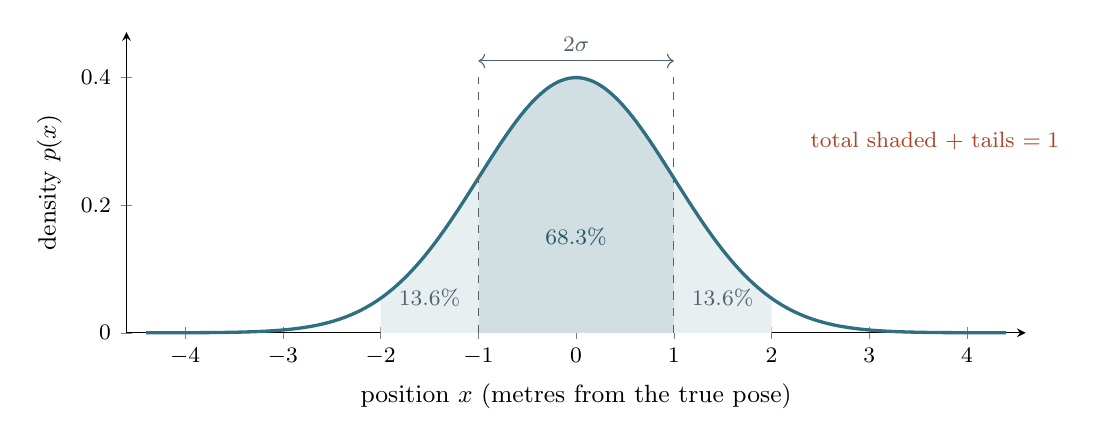
\begin{tikzpicture}[scale=1.0]
\begin{axis}[
  width=13cm, height=5.4cm,
  xmin=-4.6, xmax=4.6, ymin=0, ymax=0.47,
  axis lines=left, xlabel={position $x$ (metres from the true pose)},
  ylabel={density $p(x)$}, ylabel style={font=\small}, xlabel style={font=\small},
  tick label style={font=\footnotesize}, ytick={0,0.2,0.4},
  clip=false]
\addplot[draw=none, fill=teal!22, domain=-1:1, samples=80]
  {0.3989*exp(-x^2/2)} \closedcycle;
\addplot[draw=none, fill=teal!11, domain=-2:-1, samples=50]
  {0.3989*exp(-x^2/2)} \closedcycle;
\addplot[draw=none, fill=teal!11, domain=1:2, samples=50]
  {0.3989*exp(-x^2/2)} \closedcycle;
\addplot[teal, very thick, domain=-4.4:4.4, samples=180] {0.3989*exp(-x^2/2)};
\node[font=\footnotesize,teal!80!black] at (axis cs:0,0.15) {$68.3\%$};
\node[font=\footnotesize,slate] at (axis cs:1.5,0.055) {$13.6\%$};
\node[font=\footnotesize,slate] at (axis cs:-1.5,0.055) {$13.6\%$};
\draw[<->,slate,thin] (axis cs:-1,0.425) -- node[above,font=\footnotesize]{$2\sigma$} (axis cs:1,0.425);
\draw[dashed,slate] (axis cs:-1,0) -- (axis cs:-1,0.4);
\draw[dashed,slate] (axis cs:1,0) -- (axis cs:1,0.4);
\node[font=\footnotesize,rust,anchor=west] at (axis cs:2.3,0.30)
  {total shaded $+$ tails $=1$};
\end{axis}
\end{tikzpicture}
\caption[A probability density]{A probability density over the robot's
position error. The curve itself is not a probability; the \emph{area} under a
stretch of it is. The whole area is $1$, because the robot is somewhere. The
width parameter $\sigma$ is what AMCL reports back to us as its own confidence,
and what appears in this project's logs as \file{sigma\_x}, \file{sigma\_y} and
\file{sigma\_yaw}.}
\label{fig:density}
\end{figure}

\section{Mean, median, variance and $\sigma$}

Four summary numbers appear constantly in the results tables. Here is exactly
what each one is.

\subsection{Mean (average)}

Add the values, divide by how many there are:
\[
\bar{v} \;=\; \frac{1}{n}\sum_{i=1}^{n} v_i .
\]
For a continuous quantity the sum becomes an integral, and the mean is called
the \term{expected value}:
\begin{equation}
\mathbb{E}[X] \;=\; \int_{-\infty}^{\infty} x\, p(x)\, dx .
\label{eq:expectation}
\end{equation}
Read equation~\eqref{eq:expectation} as: \emph{go along the axis; at each
position $x$, multiply that position by how much belief sits there; add it all
up.} It is a weighted average where the weights are the density. This one
equation is the reason particle filters exist, and we will come back to it in
Part~3.

\subsection{Median}

Sort the values from smallest to largest and take the middle one. If there is
an even number of values, average the two in the middle.

\begin{handbox}[Why the results tables report medians, not means]
Consider the sixteen executed trials of the \emph{initial} run. Their true
position errors, in metres, sorted:
\[
\begin{aligned}
&0.330,\ 0.426,\ 0.467,\ 1.693,\ 2.071,\ 5.127,\ 5.182,\ \mathbf{5.202},\\
&\mathbf{7.491},\ 7.524,\ 8.733,\ 8.793,\ 11.264,\ 15.612,\ 15.631,\ 15.664 .
\end{aligned}
\]
There are $16$ values, so the median is the average of the $8$th and $9$th:
\[
\text{median} = \frac{5.202 + 7.491}{2} = \frac{12.693}{2} = \SI{6.3465}{\metre}
\;\approx\; \SI{6.35}{\metre}.
\]
That is the $\SI{6.35}{\metre}$ printed in the results table. Now compute the
mean of the same sixteen: it is $\SI{6.95}{\metre}$. The mean is dragged
upwards by the three $\SI{15}{\metre}$ failures. The median tells you what a
\emph{typical} trial looked like; the mean tells you about the worst ones. Both
are reported, deliberately.
\end{handbox}

\subsection{Variance and standard deviation}

\term{Variance} measures spread. Take each value's distance from the mean,
square it (so that being below and being above both count as spread), and
average those squares:
\[
\mathrm{Var}[X] \;=\; \mathbb{E}\!\left[(X - \mathbb{E}[X])^2\right]
\;=\; \int_{-\infty}^{\infty} \bigl(x - \mu\bigr)^2 p(x)\, dx ,
\qquad \mu = \mathbb{E}[X].
\]
Variance is in squared units --- metres squared --- which is awkward, so we
take its square root and get the \term{standard deviation}:
\[
\sigma \;=\; \sqrt{\mathrm{Var}[X]}\, .
\]
$\sigma$ is back in metres (or radians), and it is directly readable: it is
roughly ``how far off you should typically expect to be''.

\begin{keyidea}[What $\sigma_\theta = \SI{1.189}{\radian}$ means]
In this project's step-response measurement, one $\ang{90}$ turn drove the
heading standard deviation to $\SI{1.189}{\radian}$. One radian is about
$\ang{57.3}$, so $\SI{1.189}{\radian} \approx \ang{68}$. The filter was saying:
\emph{my best guess at which way the robot is pointing could easily be
$\ang{68}$ wrong.} A robot that does not know which way it is facing to within
$\ang{68}$ cannot navigate. That single number is the diagnosis of the whole
initial failure.
\end{keyidea}

\section{The Gaussian}

One density appears more than any other, because sums of many small
independent errors tend towards it. It is the \term{Gaussian} or \term{normal}
distribution, drawn in Figure~\ref{fig:density}:
\begin{equation}
\mathcal{N}(x; \mu, \sigma^2)
\;=\; \frac{1}{\sqrt{2\pi\sigma^{2}}}\,
\exp\!\left(-\frac{(x-\mu)^{2}}{2\sigma^{2}}\right).
\label{eq:gaussian}
\end{equation}

Term by term:
\begin{itemize}[leftmargin=1.4em,itemsep=2pt]
\item $\mu$ (mu) is the \textbf{centre} --- where the peak sits.
\item $\sigma$ (sigma) is the \textbf{width} --- large $\sigma$ means a broad,
low, uncertain hump; small $\sigma$ means a narrow, tall, confident spike.
\item $(x-\mu)^2$ measures how far $x$ is from the centre; dividing by
$2\sigma^2$ turns that into ``how many widths away, squared''.
\item $\exp(-\ldots)$ takes that and turns it into a number that falls off
fast --- being two widths away is much less than half as likely as being one.
\item $1/\sqrt{2\pi\sigma^2}$ is the \textbf{normalising constant}. It is
exactly the number needed to make the total area equal $1$, satisfying
equation~\eqref{eq:normalise}. Nothing about it is deep; it is bookkeeping.
\end{itemize}

The useful rule of thumb, visible in Figure~\ref{fig:density}: about $68\%$ of
the belief lies within $\pm 1\sigma$ of the centre, about $95\%$ within
$\pm 2\sigma$, and about $99.7\%$ within $\pm 3\sigma$. The number $3$ will
reappear in Part~4 as AMCL's \file{pop\_z} parameter, and that is why.

\section{Conditional probability and Bayes' rule}

This is the engine of the entire project.

\term{Conditional probability}, written $P(A \mid B)$ and read ``the
probability of $A$ \emph{given} $B$'', is the probability of $A$ once you know
that $B$ has happened. Its definition is
\[
P(A \mid B) \;=\; \frac{P(A \text{ and } B)}{P(B)} .
\]

Rearranging that definition twice --- once for $P(A\text{ and }B)$ and once for
$P(B\text{ and }A)$, which are the same thing --- gives \term{Bayes' rule}:
\begin{equation}
\boxed{\;
P(A \mid B) \;=\; \frac{P(B \mid A)\, P(A)}{P(B)}
\;}
\label{eq:bayes}
\end{equation}

The four pieces have names, and you should learn them because they are used
without explanation everywhere in robotics:
\begin{center}
\begin{tabular}{@{}lll@{}}
\toprule
\textbf{Piece} & \textbf{Name} & \textbf{In our robot} \\
\midrule
$P(A)$ & prior & what we believed about position \emph{before} the laser scan \\
$P(B \mid A)$ & likelihood & how well the scan matches the map, if we were at $A$ \\
$P(A \mid B)$ & posterior & what we believe about position \emph{after} the scan \\
$P(B)$ & evidence & the normalising divisor that makes it all sum to $1$ \\
\bottomrule
\end{tabular}
\end{center}

\begin{handbox}[Bayes' rule on a school-level example, then on the robot]
\textbf{The school example.} A test for a condition is $99\%$ accurate. The
condition affects $1$ person in $1000$. You test positive. What is the chance
you have it?

Let $A$ = ``you have it'', $B$ = ``you test positive''.
$P(A) = 0.001$. $P(B \mid A) = 0.99$. For $P(B)$, add the two ways to test
positive:
\[
P(B) = \underbrace{0.99 \times 0.001}_{\text{true positive}}
     + \underbrace{0.01 \times 0.999}_{\text{false positive}}
     = 0.00099 + 0.00999 = 0.01098 .
\]
Then
\[
P(A \mid B) = \frac{0.99 \times 0.001}{0.01098} = \frac{0.00099}{0.01098}
= 0.0902 \approx 9\% .
\]
Only $9\%$, because the condition is rare and there are far more people
available to be false positives. \textbf{This is exactly the situation the
robot was in.}

\smallskip
\textbf{The robot version, using our own initial run.} Let $A$ = ``the robot
actually arrived (within \SI{0.5}{\metre})``, $B$ = ''the stack reported
success''. Over the $16$ executed trials of the initial run: $3$ arrived, and of
those $3$, two were reported. Twelve were reported in total.
\[
P(A) = \tfrac{3}{16} = 0.1875, \qquad
P(B \mid A) = \tfrac{2}{3} = 0.667, \qquad
P(B) = \tfrac{12}{16} = 0.75 .
\]
\[
P(A \mid B) = \frac{0.667 \times 0.1875}{0.75}
= \frac{0.125}{0.75} = 0.1667 \approx 17\% .
\]
So in the initial system, hearing ``succeeded'' gave you a $17\%$ chance the
robot was really there. That number, $0.167$, is the \textbf{precision} in the
results table --- and Bayes' rule is where it comes from. Part~8 recomputes it
directly from counts and gets the same answer.
\end{handbox}

\begin{figure}[htbp]
\centering
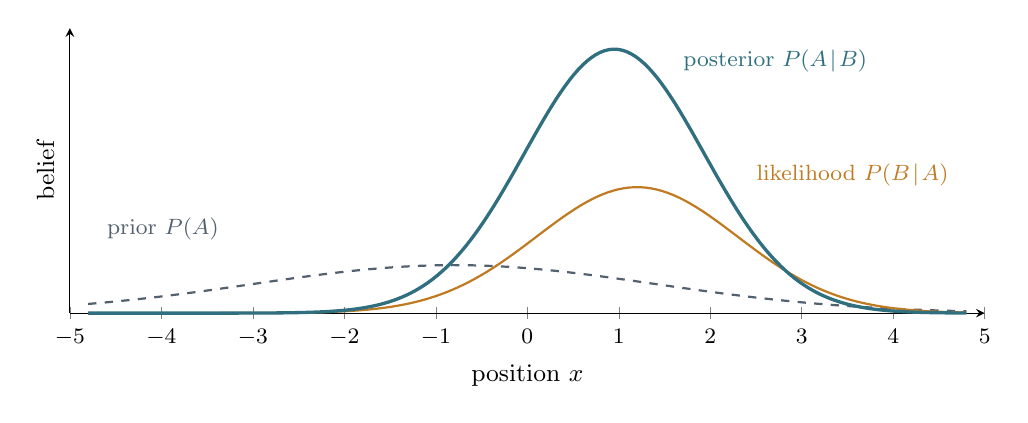
\begin{tikzpicture}[scale=1.0]
\begin{axis}[
  width=13.2cm, height=5.2cm, xmin=-5, xmax=5, ymin=0, ymax=0.95,
  axis lines=left, xlabel={position $x$}, ylabel={belief},
  xlabel style={font=\small}, ylabel style={font=\small},
  tick label style={font=\footnotesize}, ytick=\empty, clip=false]
\addplot[slate, thick, dashed, domain=-4.8:4.8, samples=160]
  {0.25*exp(-(x+0.8)^2/(2*2.2^2))/0.3989*0.3989/0.25*0.16};
\addplot[amber, thick, domain=-4.8:4.8, samples=160]
  {0.42*exp(-(x-1.2)^2/(2*1.1^2))};
\addplot[teal, very thick, domain=-4.8:4.8, samples=200]
  {0.88*exp(-(x-0.95)^2/(2*0.98^2))};
\node[slate,font=\footnotesize,anchor=west] at (axis cs:-4.7,0.28) {prior $P(A)$};
\node[amber,font=\footnotesize,anchor=west] at (axis cs:2.4,0.46) {likelihood $P(B\!\mid\!A)$};
\node[teal,font=\footnotesize,anchor=west] at (axis cs:1.6,0.84) {posterior $P(A\!\mid\!B)$};
\end{axis}
\end{tikzpicture}
\caption[Bayes' rule as a picture]{Bayes' rule, drawn. The broad dashed curve is
what we believed before the measurement. The amber curve is what the laser scan
says. Multiplying them point by point --- and then rescaling so the area is
$1$ again --- gives the taller, narrower teal curve. Every measurement makes
the belief sharper. Every movement, as we will see, makes it broader again.}
\label{fig:bayes}
\end{figure}

\section{Independence, and why it lets us multiply}

Two events are \term{independent} if knowing one tells you nothing about the
other. For independent events,
\[
P(A \text{ and } B) = P(A) \times P(B) .
\]

This matters because a laser scan is not one measurement but $120$ of them
(this project's \file{max\_beams} setting). AMCL treats the beams as
independent given the pose, so the likelihood of a whole scan
$\mathbf{z} = \{z_1,\ldots,z_{120}\}$ is the product of the individual beam
likelihoods:
\begin{equation}
p(\mathbf{z} \mid \xt, m) \;=\; \prod_{k=1}^{120} p(z_k \mid \xt, m),
\label{eq:beamproduct}
\end{equation}
where $\prod$ means ``multiply all of these together'', $\xt$ is the pose being
tested, and $m$ is the map.

\begin{warnbox}[Independence here is a convenient fiction]
Neighbouring laser beams hitting the same flat wall are obviously \emph{not}
independent --- if one is long, its neighbour almost certainly is too.
Multiplying them anyway makes the resulting likelihood far too confident, too
peaked. This is a known and accepted approximation in every implementation of
this algorithm, and it is one reason a filter can lock onto a wrong hypothesis
with great conviction. It is also part of why this project caps the scan at
$120$ beams out of the $720$ available rather than using all of them: fewer,
more widely spaced beams are closer to independent.
\end{warnbox}

% =========================================================================
\chapter{The robot's problem: where am I?}
\label{ch:where}

\section{Two different jobs: building the map, and using it}
\label{sec:slam-vs-amcl}

Before anything else, a distinction that causes more confusion than any other
in this subject, because the two things use the same sensors, produce the same
kind of answer, and are almost always drawn in the same diagram.

\begin{keyidea}[The question is whether you already have a map]
\textbf{SLAM} --- Simultaneous Localisation And Mapping --- is the problem you
have when there is \emph{no} map. You must work out where the robot is
\emph{and} draw the building, at the same time, from the same data. Each
answer depends on the other, which is what makes it hard.

\textbf{Localisation} is the problem you have when the map already exists. The
building is given. All you have to find is the robot inside it.

This project does both --- but never at the same time, and never in the same
run.
\end{keyidea}

\subsection{Phase 1: mapping, done once}

The robot was driven around the house by hand while \file{slam\_toolbox} was
running. At that moment no map existed. \file{slam\_toolbox} produced both the
map and the trajectory, and the finished occupancy grid was saved to disk as
\file{custom\_map\_v2.pgm}. Then that phase ended, permanently. It is not
repeated for experiments.

\subsection{Phase 2: operation, every single trial in this study}

\file{slam\_toolbox} is not running. A node called \file{map\_server} loads
the saved \file{.pgm} file, and \file{amcl} finds the robot inside it. Every
number in Part~8 of this document comes from this phase. Nothing in the
results measures SLAM.

\begin{warnbox}[They cannot both run]
Only one node in a ROS system is allowed to publish the
$\text{map} \rightarrow \text{odom}$ transform (\S2.2 explains what that is).
Both \file{slam\_toolbox} and \file{amcl} want to publish it. So you run one or
the other. There is no configuration in which they cooperate.
\end{warnbox}

\subsection{Filtering and smoothing --- the difference that explains the results}

There is a second distinction hiding underneath the first, and it is the one
that actually explains why this project's errors look the way they do.

\begin{center}
\small
\begin{tabular}{@{}p{0.44\textwidth}p{0.44\textwidth}@{}}
\toprule
\textbf{Filtering} & \textbf{Smoothing} \\
\midrule
Estimates the state \emph{now}, from the latest measurement.
& Estimates the \emph{whole trajectory}, using every measurement ever taken. \\[4pt]
Keeps one answer and moves it forward.
& Keeps all the answers and adjusts them together. \\[4pt]
Cannot revisit a past mistake --- the past is not stored.
& Can go back and correct the past when new evidence arrives. \\[4pt]
Cheap, constant work per step.
& Expensive, and grows as the trajectory grows. \\[4pt]
Examples: Kalman filter, extended Kalman filter, \textbf{particle filter}.
& Examples: \textbf{pose-graph optimisation}, bundle adjustment. \\
\midrule
\textbf{This project: AMCL, every trial.}
& \textbf{This project: \file{slam\_toolbox}, when the map was built.} \\
\bottomrule
\end{tabular}
\end{center}

\textbf{How smoothing actually works.} A pose graph is a picture of the
robot's history. Each \term{node} is a pose the robot occupied. Each
\term{edge} is a measured relationship between two poses --- ``from here, I
moved forward \SI{0.8}{\metre} and turned \ang{10}''. Odometry supplies edges
between consecutive poses, and those edges accumulate error, so the drawn
trajectory slowly bends away from the truth.

Then comes the event that makes the whole thing work. The robot returns
somewhere it has already been, and the laser recognises it. That is a
\term{loop closure}, and it adds an edge between two nodes that are far apart
in time. Now the graph is over-determined: it contains a cycle whose edges do
not quite agree. \term{Pose-graph optimisation} --- solved here by the Ceres
library --- moves \emph{every} node a little so that the disagreement is
spread evenly around the loop instead of piling up at one end. Poses recorded
minutes ago are silently corrected by something observed just now.

\begin{keyidea}[Why this matters for Part~8]
A smoother can be wrong and then stop being wrong. A filter can only be wrong
and stay wrong.

AMCL is a filter. It holds a belief about where the robot is \emph{right now}
and nothing else. Once its particles have crowded onto the wrong hypothesis,
there is no stored past to re-examine and no mechanism to reconsider --- and
the crowding itself has thrown away the particles that were near the right
answer. This is the whole reason the failures in this study are not merely
large but \emph{stable}: in \S\ref{sec:hand-distance} you will see three
separate runs to the same room finish \SI{15.6}{\metre} from the goal and
agree with each other to \SI{0.05}{\metre}. The filter was not lost and
wandering. It was confidently, consistently, repeatably in the wrong place.

\S5.5 covers the one escape hatch AMCL provides for this, and why it is
switched off here.
\end{keyidea}

\section{Three frames, and the seam between them}

A robot cannot talk about ``position'' without saying \emph{position measured
from what}. A \term{frame} is an origin plus a set of axes. This project uses
three, and understanding the relationship between them explains almost every
failure that was diagnosed.

\begin{plain}[The three frames]
\begin{description}[leftmargin=2.6cm,style=nextline,font=\ttfamily\color{teal}]
\item[base\_link] Attached to the robot itself. Its origin sits between the
drive wheels; $x$ points forward. When the robot moves, this frame moves with
it. Everything mounted on the robot --- the laser, the camera --- is described
relative to \file{base\_link}.
\item[odom] A fixed frame the robot invents when it switches on. It is
\emph{smooth}: the robot's position in \file{odom} never jumps, it only ever
changes a little bit at a time. But it \emph{drifts}: after driving for a
while, \file{odom} no longer lines up with the real world.
\item[map] The world frame, tied to the building. It does \emph{not} drift.
But the robot's position in \file{map} can jump, because it is inferred rather
than integrated.
\end{description}
\end{plain}

These are chained together. In ROS the chain is
\[
\texttt{map} \;\longrightarrow\; \texttt{odom} \;\longrightarrow\;
\texttt{base\_link}.
\]

\begin{figure}[htbp]
\centering
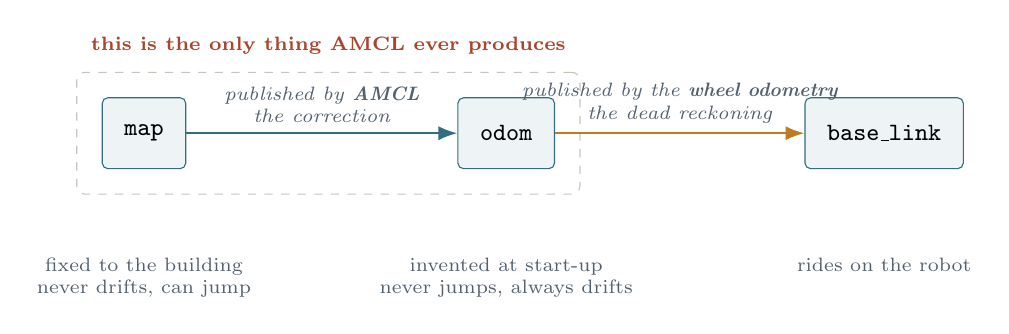
\begin{tikzpicture}[
  font=\small,
  frame/.style={draw=teal,fill=teal!8,rounded corners=2pt,minimum height=9mm,
                inner xsep=8pt,font=\ttfamily\small},
  lbl/.style={font=\scriptsize\itshape,color=slate}]
\node[frame] (map) at (0,0) {map};
\node[frame] (odom) at (4.6,0) {odom};
\node[frame] (base) at (9.4,0) {base\_link};
\draw[-{Latex[length=2.4mm]},teal,thick] (map) -- node[above,lbl,align=center]
  {published by \textbf{AMCL}\\the correction} (odom);
\draw[-{Latex[length=2.4mm]},amber,thick] (odom) -- node[above,lbl,align=center]
  {published by the \textbf{wheel odometry}\\the dead reckoning} (base);
\node[below=10mm of map,align=center,font=\scriptsize,color=slate]
  {fixed to the building\\never drifts, can jump};
\node[below=10mm of odom,align=center,font=\scriptsize,color=slate]
  {invented at start-up\\never jumps, always drifts};
\node[below=10mm of base,align=center,font=\scriptsize,color=slate]
  {rides on the robot};
\begin{scope}[on background layer]
\node[draw=rule,dashed,rounded corners=3pt,inner sep=9pt,
      fit=(map)(odom),label={[font=\scriptsize\bfseries,color=rust,yshift=1mm]above:this
      is the only thing AMCL ever produces}] {};
\end{scope}
\end{tikzpicture}
\caption[The TF chain]{The transform chain. The wheel odometry supplies
\texttt{odom}$\rightarrow$\texttt{base\_link} by counting wheel rotations.
AMCL supplies \texttt{map}$\rightarrow$\texttt{odom}, and \emph{that transform
is its entire output}. AMCL never moves the robot and never tells anyone where
the robot is directly; it silently adjusts the offset between the drifting
frame and the true one. Nav2 reads the composed chain and never has to know
AMCL exists. Part~6 shows why that seam is where the project's headline fault
was hiding.}
\label{fig:tf}
\end{figure}

\begin{figure}[htbp]
\centering
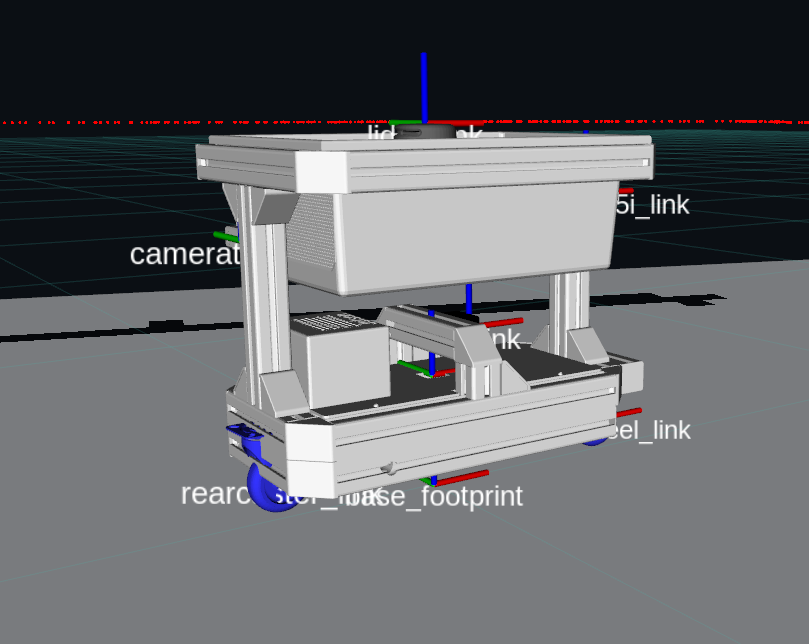
\includegraphics[width=0.68\textwidth]{fig/rviz_frames.png}
\caption[The frames on the robot]{The ROMR model in RViz with its coordinate
frames drawn. Each little red--green--blue triad is one frame: red is $x$,
green is $y$, blue is $z$. \file{base\_footprint} sits on the ground between
the wheels, \file{base\_link} on the chassis above it, and the sensor frames
(\file{camera\_link}, the lidar frame) are fixed offsets from it. These
relationships come from the URDF and never change. The two that \emph{do}
change --- \texttt{map}$\rightarrow$\texttt{odom} and
\texttt{odom}$\rightarrow$\texttt{base\_link} --- are the ones in
Figure~\ref{fig:tf}, and they are the entire subject of this document.}
\label{fig:rvizframes}
\end{figure}

\begin{keyidea}
AMCL's job is not ``find the robot''. Its job is ``compute the correction that
must be applied to the drifting odometry frame so that the composed result
matches the map''. Everything else in the navigation stack reads the composed
result and takes it on trust.
\end{keyidea}

\section{Odometry: counting wheel turns}

ROMR is a \term{differential-drive} robot: two independently driven wheels on
a common axle, plus passive casters for balance. From the Gazebo plugin
configuration used in this project (\file{romr\_gazebo\_plugins.gazebo}):

\begin{center}
\begin{tabular}{@{}lll@{}}
\toprule
\textbf{Quantity} & \textbf{Symbol} & \textbf{Value in this project} \\
\midrule
Wheel separation (track width) & $L$ & \SI{0.2937}{\metre} \\
Wheel diameter                 & $2r$& \SI{0.1627}{\metre} \\
Wheel radius                   & $r$ & \SI{0.08135}{\metre} \\
Odometry publication rate      & --- & \SI{50}{\hertz} \\
\bottomrule
\end{tabular}
\end{center}

If the left wheel turns at angular rate $\omega_L$ and the right at
$\omega_R$ (radians per second), their contact points move at
$v_L = r\,\omega_L$ and $v_R = r\,\omega_R$. The robot's body then has
\begin{equation}
v \;=\; \frac{v_R + v_L}{2}, \qquad\qquad
\omega \;=\; \frac{v_R - v_L}{L},
\label{eq:diffdrive}
\end{equation}
where $v$ is forward speed in \si{\metre\per\second} and $\omega$ is turning
rate in \si{\radian\per\second}.

Read equation~\eqref{eq:diffdrive} in words. \emph{Forward speed is the
average of the two wheels} --- if both go forward at the same speed, the robot
goes forward and does not turn. \emph{Turning rate is the difference divided
by the track width} --- if the right wheel outruns the left, the robot swings
left, and the narrower the robot, the faster it swings for the same
difference.

To get position we \term{integrate}: we add up all the little movements. Over
a short interval $\Delta t$,
\begin{equation}
\begin{aligned}
\theta_{t+1} &= \theta_t + \omega\,\Delta t, \\
x_{t+1} &= x_t + v\,\Delta t\,\cos\theta_t, \\
y_{t+1} &= y_t + v\,\Delta t\,\sin\theta_t .
\end{aligned}
\label{eq:deadreckon}
\end{equation}
Doing this repeatedly is called \term{dead reckoning}.

\begin{handbox}[Odometry by hand, with this robot's real dimensions]
Suppose over one \SI{50}{\hertz} tick ($\Delta t = \SI{0.02}{\second}$) the
left wheel spins at $\omega_L = \SI{3.0}{\radian\per\second}$ and the right at
$\omega_R = \SI{5.0}{\radian\per\second}$.

\smallskip
\textbf{Step 1 --- wheel surface speeds.}
\[
v_L = 0.08135 \times 3.0 = \SI{0.24405}{\metre\per\second}, \qquad
v_R = 0.08135 \times 5.0 = \SI{0.40675}{\metre\per\second}.
\]

\textbf{Step 2 --- body speeds, from equation~\eqref{eq:diffdrive}.}
\[
v = \frac{0.40675 + 0.24405}{2} = \frac{0.6508}{2} = \SI{0.3254}{\metre\per\second},
\]
\[
\omega = \frac{0.40675 - 0.24405}{0.2937} = \frac{0.1627}{0.2937}
= \SI{0.5540}{\radian\per\second}.
\]

\textbf{Step 3 --- one tick of motion.} Starting at
$(x,y,\theta) = (0,0,0)$:
\[
\theta_{1} = 0 + 0.5540 \times 0.02 = \SI{0.01108}{\radian}\ (\ang{0.635}),
\]
\[
x_{1} = 0 + 0.3254 \times 0.02 \times \cos 0 = \SI{0.006508}{\metre},
\qquad y_1 = 0 .
\]

\textbf{Step 4 --- why this goes wrong.} Now suppose the wheel radius is
really $\SI{0.0805}{\metre}$, not $\SI{0.08135}{\metre}$ --- a $1\%$ error,
completely invisible. Every $v$ is $1\%$ too big. After the robot has driven
$\SI{20}{\metre}$, dead reckoning reports $\SI{20.2}{\metre}$: a
$\SI{0.2}{\metre}$ error that will never be corrected, because
equation~\eqref{eq:deadreckon} only ever \emph{adds}. Errors accumulate and
never cancel. This is why \file{odom} drifts and why we need everything that
follows.
\end{handbox}

\subsection{Why rotation is the enemy on this robot}

ROMR's casters are \emph{fixed}, not swivelling. When the robot rotates in
place, the casters cannot roll in the direction they are being dragged, so
they \emph{scrub} sideways across the floor --- measured in this project at
$\SI{180}{\milli\metre}$ to $\SI{220}{\milli\metre}$ per turn. The wheel
encoders happily report that the drive wheels turned exactly as commanded,
because they did. What they cannot report is that the whole chassis also slid.

That produces a distinctive signature, which this project measured directly:

\begin{center}
\begin{tabular}{@{}lccc@{}}
\toprule
\textbf{Condition} & $e$ (\si{\metre}) & $\Delta\theta$ (\si{\degree}) & $\sigma_\theta$ (\si{\radian}) \\
\midrule
Immediately after seeding from ground truth & 0.014 & $-0.1$ & 0.128 \\
After \SI{8}{\second} standing still        & 0.015 & $-0.1$ & 0.128 \\
After one \ang{90} turn                     & 0.159 & $-17.4$& \textbf{1.189} \\
After turning back                          & 0.577 & $-24.9$& 1.233 \\
After \SI{0.8}{\metre} forward              & 0.736 & $-36.5$& 1.105 \\
After \SI{0.8}{\metre} reverse              & 0.289 & $-26.8$& 0.883 \\
\bottomrule
\end{tabular}
\end{center}

Standing still costs nothing. Driving straight costs a little and actually
pulls $\sigma_\theta$ back \emph{down}. One rotation multiplies $\sigma_\theta$
by $1.189/0.128 = 9.3$.

\section{The belief, and the Bayes filter}

Because the robot cannot know its pose, it maintains a whole density over
poses. Write the pose at time $t$ as
$\xt_t = (x_t, y_t, \theta_t)$, the control (commanded motion) as $u_t$, the
sensor reading as $z_t$, and the map as $m$. The \term{belief} is
\begin{equation}
\mathrm{bel}(\xt_t) \;=\; p\bigl(\xt_t \,\big|\, z_{1:t},\, u_{1:t},\, m\bigr),
\label{eq:belief}
\end{equation}
read as: \emph{the density over where I might be, given every sensor reading
and every command since I switched on, and given the map.}

The \term{Bayes filter} updates this belief in two alternating steps, forever.

\subsection{Step 1 --- Prediction (the robot moved)}

Before the new sensor reading arrives, account for the commanded motion:
\begin{equation}
\overline{\mathrm{bel}}(\xt_t)
\;=\; \int p\bigl(\xt_t \mid u_t, \xt_{t-1}\bigr)\;
              \mathrm{bel}(\xt_{t-1})\; d\xt_{t-1} .
\label{eq:predict}
\end{equation}

This integral is worth reading slowly, because it is the heart of everything.

\begin{plain}[Equation~\eqref{eq:predict} in plain words]
``To work out how strongly I should believe I am now at pose $\xt_t$, consider
\emph{every} pose $\xt_{t-1}$ I might have been at a moment ago. For each one,
multiply (a) how strongly I believed I was there,
$\mathrm{bel}(\xt_{t-1})$, by (b) the chance that the commanded motion $u_t$
would have carried me from there to here,
$p(\xt_t \mid u_t, \xt_{t-1})$. Then add up all those contributions.''

The $\int \ldots d\xt_{t-1}$ is that ``add up over every possible previous
pose''. The term $p(\xt_t \mid u_t, \xt_{t-1})$ is the \term{motion model} ---
it is where wheel slip, caster scrub and encoder error are admitted.

The consequence: because the motion model is uncertain, this step always makes
the belief \emph{broader}. Moving makes you less sure.
\end{plain}

\subsection{Step 2 --- Correction (the laser saw something)}

Now fold in the measurement, using Bayes' rule~\eqref{eq:bayes}:
\begin{equation}
\mathrm{bel}(\xt_t) \;=\; \eta \; p\bigl(z_t \mid \xt_t, m\bigr)\;
\overline{\mathrm{bel}}(\xt_t),
\qquad
\eta = \frac{1}{\displaystyle\int p(z_t \mid \xt_t, m)\,\overline{\mathrm{bel}}(\xt_t)\,d\xt_t}.
\label{eq:correct}
\end{equation}

$p(z_t \mid \xt_t, m)$ is the \term{measurement model} or \term{likelihood}:
given the map, and supposing the robot were at $\xt_t$, how plausible is the
scan we just received? Poses that would have produced this scan get their
belief multiplied up; poses that would not get theirs multiplied down.

$\eta$ (eta) is just the normaliser from equation~\eqref{eq:normalise}: divide
by the total so the area comes back to $1$. It carries no information.

\begin{keyidea}[The whole of localisation, in one sentence]
\emph{Movement spreads the belief out; measurement pulls it back in.} A robot
localises successfully when measurement can pull in faster than movement
spreads out. Every parameter this project tuned is a parameter that changes the
balance of that race --- and Part~5 identifies which side of the race each one
sits on.
\end{keyidea}

\subsection{Why we cannot just compute this}

Equations~\eqref{eq:predict} and \eqref{eq:correct} are exact and complete. If
we could evaluate them we would be finished. We cannot, for two reasons.

First, $\xt$ is three-dimensional and continuous. To store
$\mathrm{bel}(\xt)$ on a grid fine enough to be useful --- say
\SI{5}{\centi\metre} and \ang{5} --- over this project's
$\SI{13.9}{\metre} \times \SI{11.6}{\metre}$ building, you would need roughly
$278 \times 232 \times 72 \approx 4.6$ million cells, updated at
\SI{20}{\hertz}. That is possible but wasteful, since almost all of those
cells hold essentially zero.

Second, the integral in equation~\eqref{eq:predict} has no closed-form
solution for a realistic motion model. There is no formula to write down.

So we approximate. The approximation is the subject of Part~3.

% =========================================================================
\chapter{Monte Carlo: a belief made of dots}
\label{ch:mc}

\section{The idea: replace a curve with a crowd}

Instead of storing the belief as a function, store it as a \emph{crowd of
guesses}. Each guess is a complete hypothesis about the robot's pose --- an
$(x, y, \theta)$ triple --- and it is called a \term{particle}. Where the true
belief is high, we put many particles; where it is low, we put few.

Formally, the belief is represented by a set of $J$ weighted particles:
\begin{equation}
\mathcal{X}_t \;=\; \Bigl\{\; \bigl\langle \xt_t^{[j]},\; w_t^{[j]} \bigr\rangle
\;\Bigr\}_{j=1,\ldots,J},
\qquad \sum_{j=1}^{J} w_t^{[j]} = 1 .
\label{eq:particleset}
\end{equation}
The superscript $[j]$ labels which particle; $w^{[j]}$ is that particle's
\term{weight}, its share of the total belief.

In this project $J$ is not fixed: it varies between $500$ and $2000$, for
reasons explained in Part~4 \S4.4.

\begin{figure}[htbp]
\centering
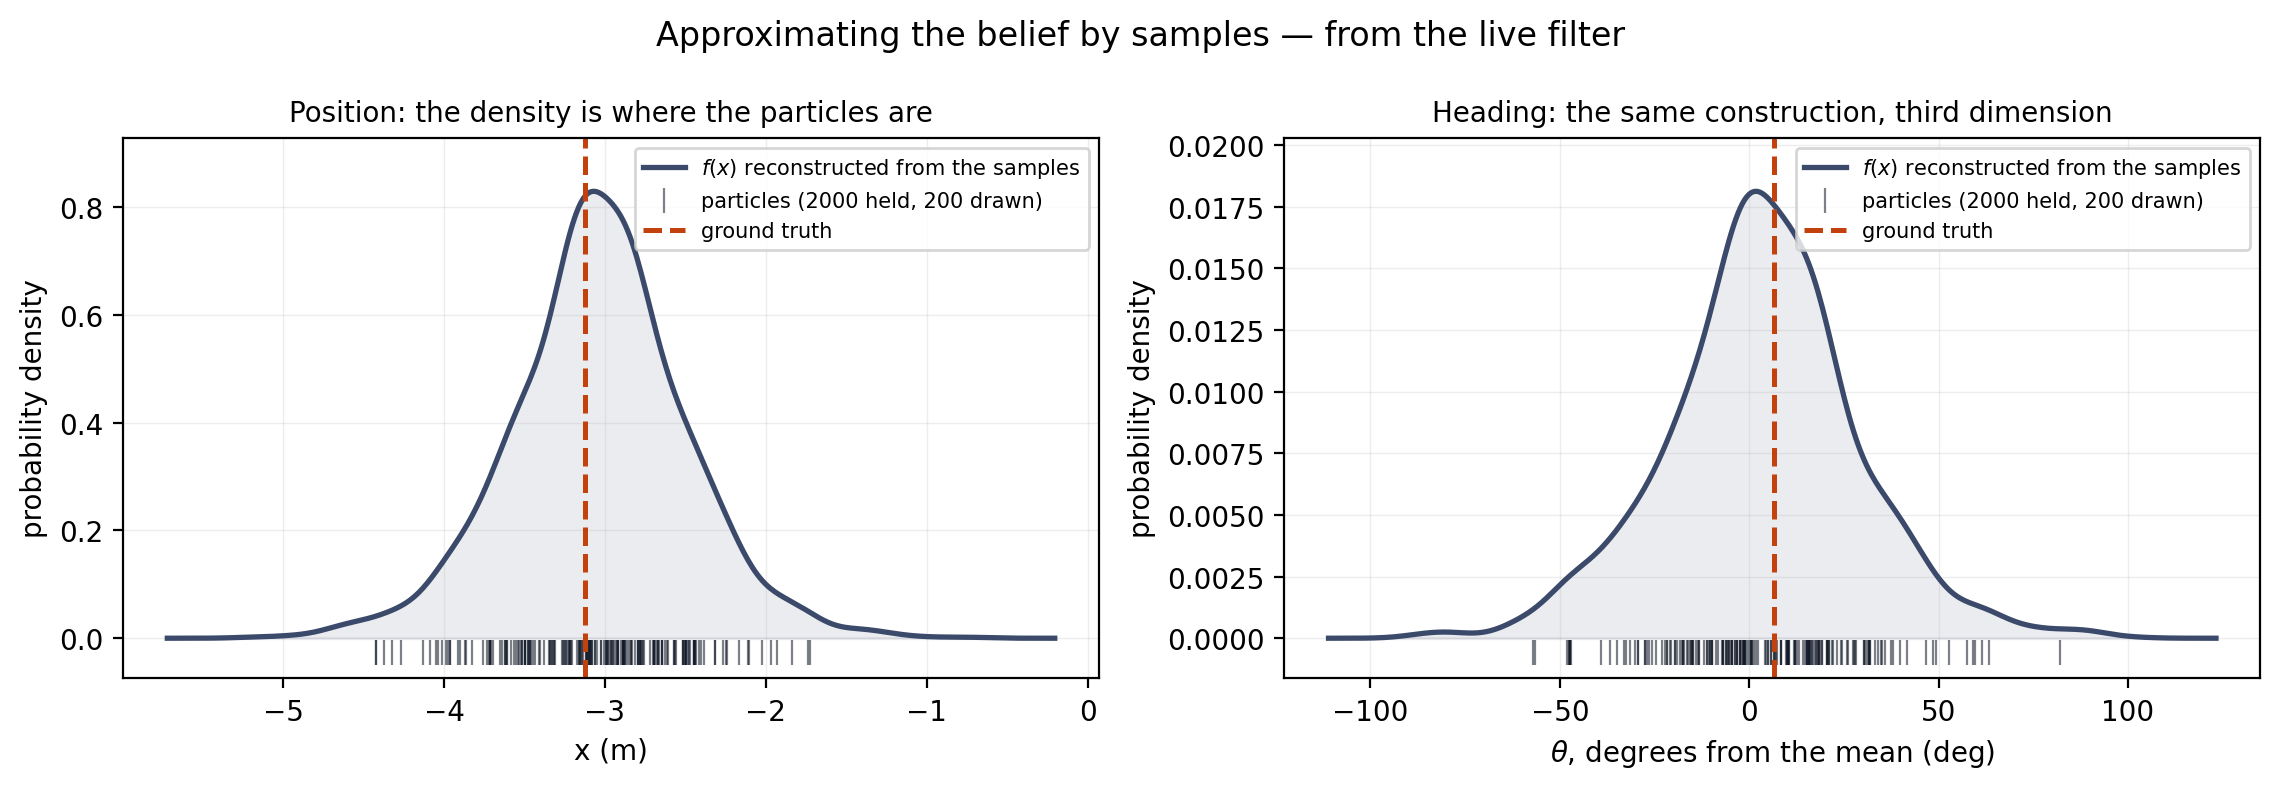
\includegraphics[width=\textwidth]{fig/p_approx.png}
\caption[A density approximated by particles]{The same belief written two
ways. Left: as a smooth density, the thing we cannot compute. Right: as a
crowd of particles, the thing we can. Where the curve is tall, the dots are
dense. This figure was generated for this project by
\file{scripts/particle\_approx\_figure.py}.}
\label{fig:papprox}
\end{figure}

\section{Importance sampling: the mathematics that makes it legal}

Why is a crowd of dots a legitimate stand-in for an integral? The answer is
\term{importance sampling}, and it is worth doing properly because the whole
evaluation strategy of this project descends from it.

\subsection{The problem}

We want an expectation --- an average of some quantity $f(\xt)$ under the
belief $p$:
\begin{equation}
\mathbb{E}_p[f] \;=\; \int f(\xt)\, p(\xt)\, d\xt .
\label{eq:target}
\end{equation}
For example, if $f(\xt) = x$, this gives the robot's mean $x$ coordinate ---
exactly the number AMCL publishes on \file{/amcl\_pose}.

The trouble: we cannot draw samples from $p$. We do not have $p$ in a form we
can sample from; that is the whole difficulty.

\subsection{The trick}

Suppose there \emph{is} some other density $\pi(\xt)$ that we \emph{can}
sample from --- call it the \term{proposal}. Multiply and divide
equation~\eqref{eq:target} by it:
\begin{equation}
\mathbb{E}_p[f]
\;=\; \int f(\xt)\, p(\xt)\, d\xt
\;=\; \int f(\xt)\, \frac{p(\xt)}{\pi(\xt)}\, \pi(\xt)\, d\xt
\;=\; \mathbb{E}_{\pi}\!\left[\, f(\xt)\, \frac{p(\xt)}{\pi(\xt)} \,\right].
\label{eq:importance}
\end{equation}

Nothing has been assumed and nothing has been lost --- we multiplied by
$\pi/\pi = 1$. But the meaning has changed completely. The left-hand side is
an average under a density we cannot sample. The right-hand side is an average
under a density we \emph{can} sample, of a slightly different quantity.

Define the \term{importance weight}
\begin{equation}
w(\xt) \;=\; \frac{p(\xt)}{\pi(\xt)}
\;=\; \frac{\text{how much belief truly belongs here}}
            {\text{how often we actually generate samples here}} .
\label{eq:weightdef}
\end{equation}

Then draw $J$ samples $\xt^{[j]} \sim \pi$ and estimate
\begin{equation}
\mathbb{E}_p[f] \;\approx\;
\frac{\sum_{j=1}^{J} w(\xt^{[j]})\, f(\xt^{[j]})}
     {\sum_{j=1}^{J} w(\xt^{[j]})} .
\label{eq:selfnorm}
\end{equation}
(The division by $\sum w$ is the self-normalising form; it is what lets us get
away with knowing $p$ only up to a constant, which is all
equation~\eqref{eq:correct} ever gives us, because $\eta$ is unknown.)

\begin{keyidea}[The one-sentence version]
\emph{Sample from wherever is convenient, then correct for having sampled from
the wrong place by weighting each sample by how wrong the place was.}
\end{keyidea}

\subsection{The precondition nobody mentions, and why it matters here}

Equation~\eqref{eq:importance} requires that
\begin{equation}
p(\xt) > 0 \;\Longrightarrow\; \pi(\xt) > 0 .
\label{eq:support}
\end{equation}
The proposal must be able to generate samples \emph{everywhere the truth might
be}. If $\pi$ is zero somewhere that $p$ is not, the weight
$p/\pi$ becomes division by zero --- and in practice, the estimator simply
never sees that region and reports with total confidence about a place the
robot is not.

\begin{warnbox}[This is precisely the failure that was measured]
In the initial run, the robot's belief converged tightly ($\sigma$ small,
$e_{\text{AMCL}}$ typically under \SI{0.4}{\metre}) onto a pose that was up to
\SI{15.66}{\metre} from the truth. Not one particle was near the real robot.
The estimator was not ``noisy'' --- it was \emph{confidently answering a
different question}, exactly as equation~\eqref{eq:support} warns. No amount of
averaging fixes a violated support condition. This is why the corrected system
addresses the \emph{model}, not the number of particles.
\end{warnbox}

\section{The three steps of a particle filter}

Each cycle of the filter does prediction, correction, and one extra step
that has no counterpart in the exact Bayes filter.

\begin{plain}[The algorithm]
Given the previous particle set $\mathcal{X}_{t-1}$, the control $u_t$, the
scan $z_t$ and the map $m$:

\smallskip
\textbf{Step 1 --- Sample (prediction).} For each particle $j$:
\[
\xt_t^{[j]} \;\sim\; p\bigl(\xt_t \mid u_t,\, \xt_{t-1}^{[j]}\bigr).
\]
Move every particle according to the odometry, plus a random perturbation
drawn from the motion model. This is the Monte Carlo version of the integral
in equation~\eqref{eq:predict}: instead of integrating over all previous
poses, we push each of our $J$ samples through the motion.

\smallskip
\textbf{Step 2 --- Weight (correction).} For each particle $j$:
\[
w_t^{[j]} \;=\; p\bigl(z_t \mid \xt_t^{[j]},\, m\bigr),
\quad\text{then normalise}\quad
w_t^{[j]} \leftarrow \frac{w_t^{[j]}}{\sum_{k} w_t^{[k]}} .
\]
Ask each particle: ``if the robot really were at your pose, how likely is the
scan we just received?'' That number is its weight. This is
equation~\eqref{eq:correct}, and the normalisation is $\eta$.

\smallskip
\textbf{Step 3 --- Resample.} Draw $J$ new particles from the current set,
\emph{with replacement}, choosing particle $j$ with probability $w^{[j]}$.
Set all new weights to $1/J$.
\end{plain}

\subsection{Why Step 3 is necessary}

Without resampling, after a few dozen cycles one particle holds a weight of
essentially $1$ and all the others hold essentially $0$. You are then paying
for $J$ particles and getting the statistical value of one. This is called
\term{weight degeneracy}. Resampling kills off the low-weight particles and
duplicates the high-weight ones, so that the \emph{density of particles}
carries the information that the \emph{weights} used to carry.

Notice the exchange: before resampling, belief lives in the weights; after
resampling, all weights are equal and belief lives in where the particles are.

\begin{warnbox}[Resampling introduces its own disease]
Duplicating particles destroys diversity. Run resampling often enough with no
new information and every particle becomes a copy of one ancestor --- this is
\term{particle depletion} or \term{sample impoverishment}. If the true pose was
not among the survivors, it can never be recovered, because Step~1 only ever
jitters existing particles; it never invents new ones far away.

This project sets \file{resample\_interval: 1}, meaning it resamples on
\emph{every} filter update. That is the most aggressive setting and it makes
depletion a live concern. It is one of the tuning levers identified in
Part~11.
\end{warnbox}

\section{Seeing it happen on this robot}

The following four figures were produced from this project's own filter, using
\file{scripts/particle\_figure.py}, and they show the mechanism directly.

\begin{figure}[htbp]
\centering
\begin{minipage}{0.49\textwidth}\centering
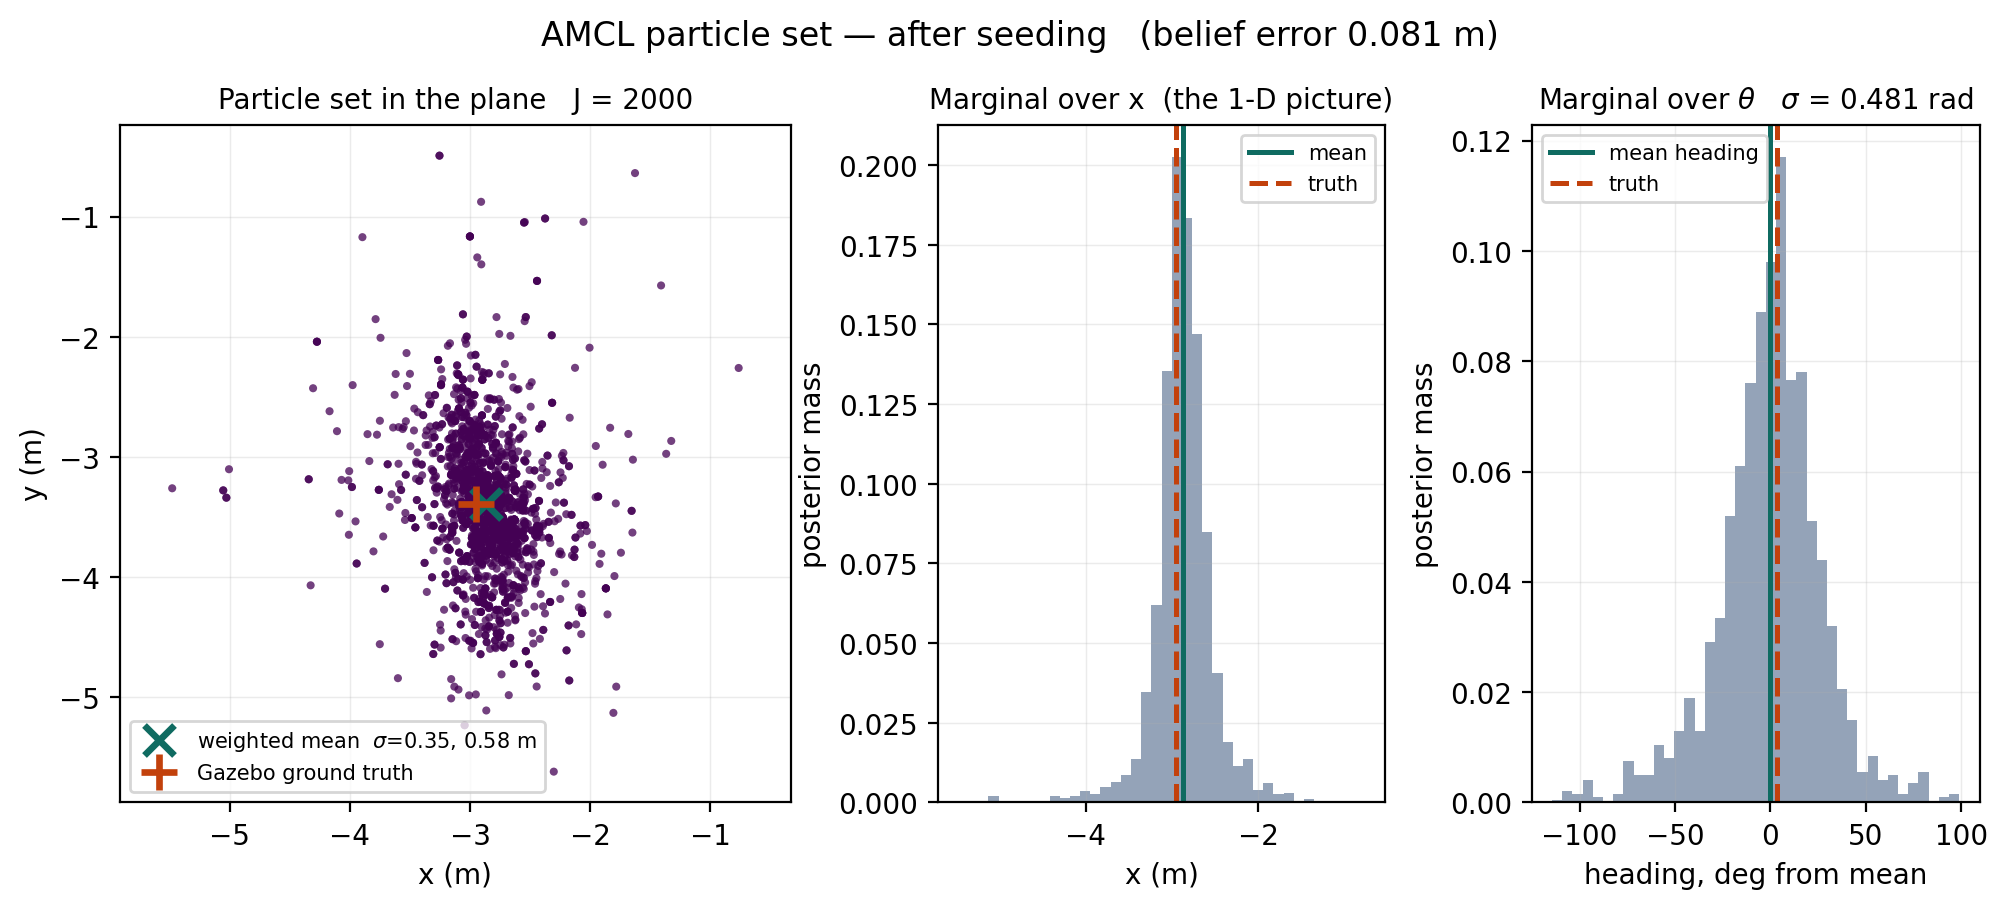
\includegraphics[width=\textwidth]{fig/p1_seeded.png}\\[2pt]
{\footnotesize (a) immediately after seeding from ground truth}
\end{minipage}\hfill
\begin{minipage}{0.49\textwidth}\centering
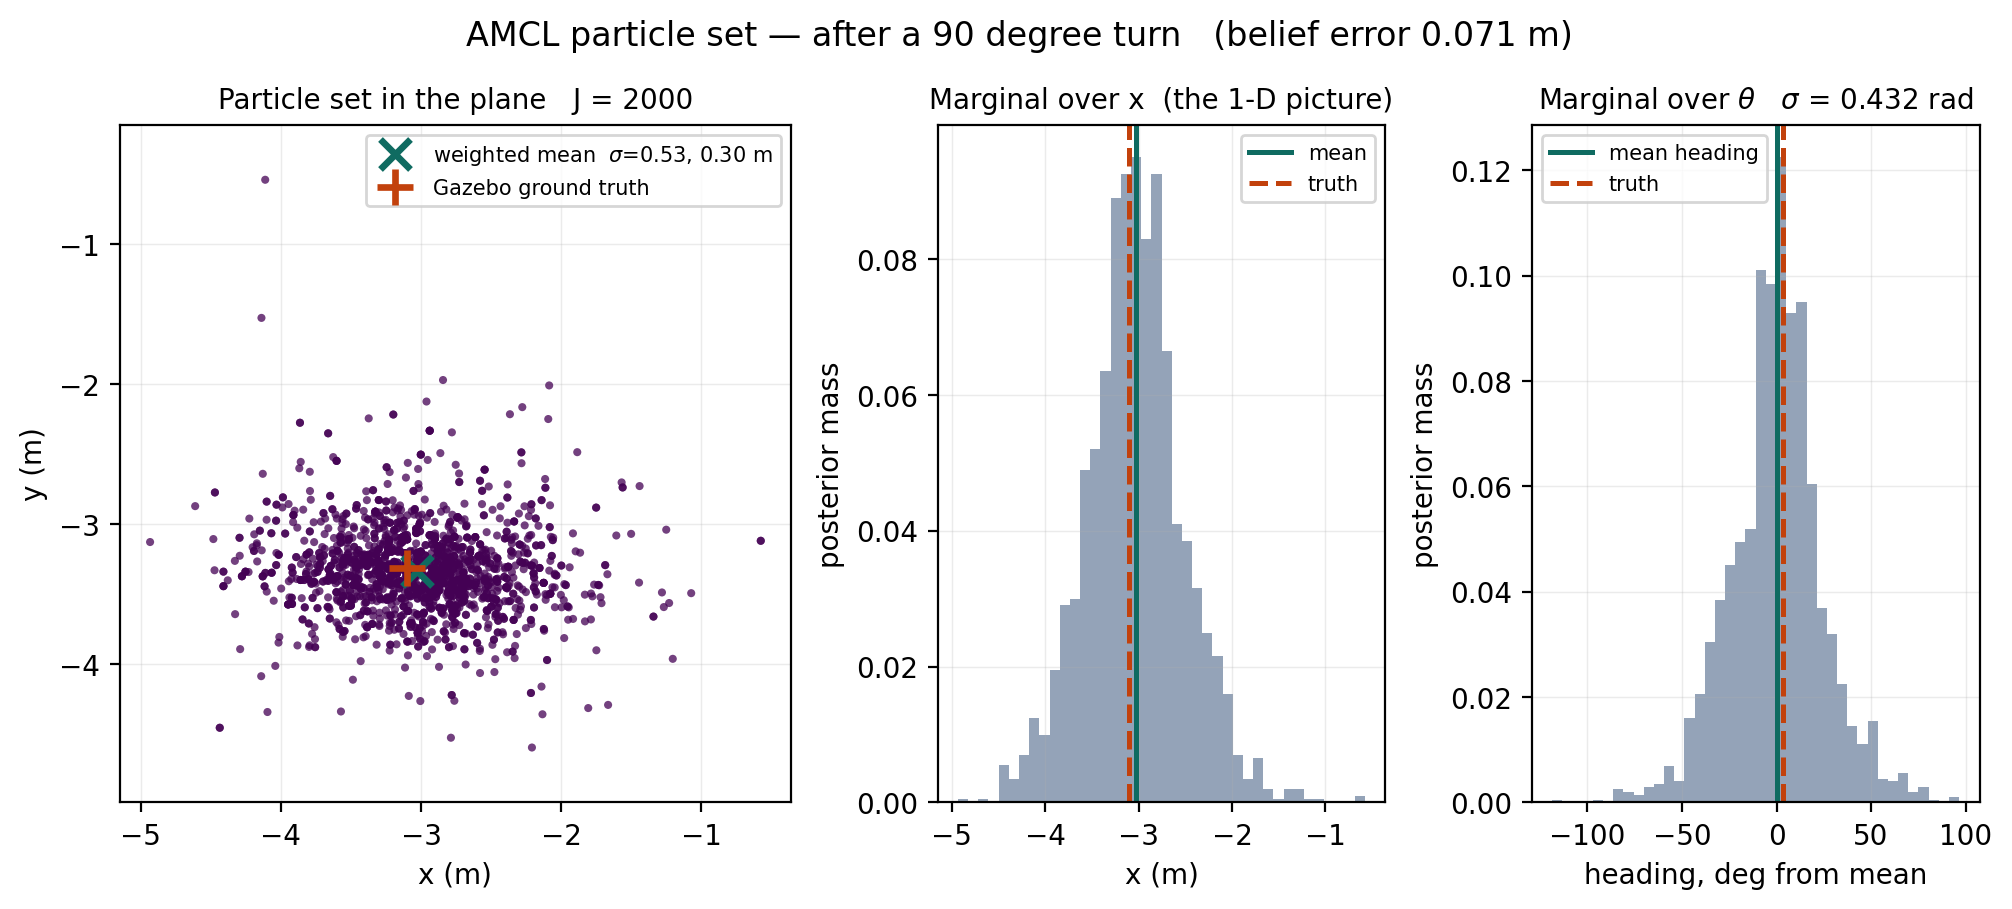
\includegraphics[width=\textwidth]{fig/p2_turn.png}\\[2pt]
{\footnotesize (b) after a single \ang{90} turn, tuned filter}
\end{minipage}
\caption[Particle cloud, tuned]{The particle cloud with the corrected
parameters. Seeding places a tight cluster on the true pose. One rotation
spreads it --- prediction always spreads --- but the scan correction holds it
together.}
\label{fig:cloud-good}
\end{figure}

\begin{figure}[htbp]
\centering
\begin{minipage}{0.49\textwidth}\centering
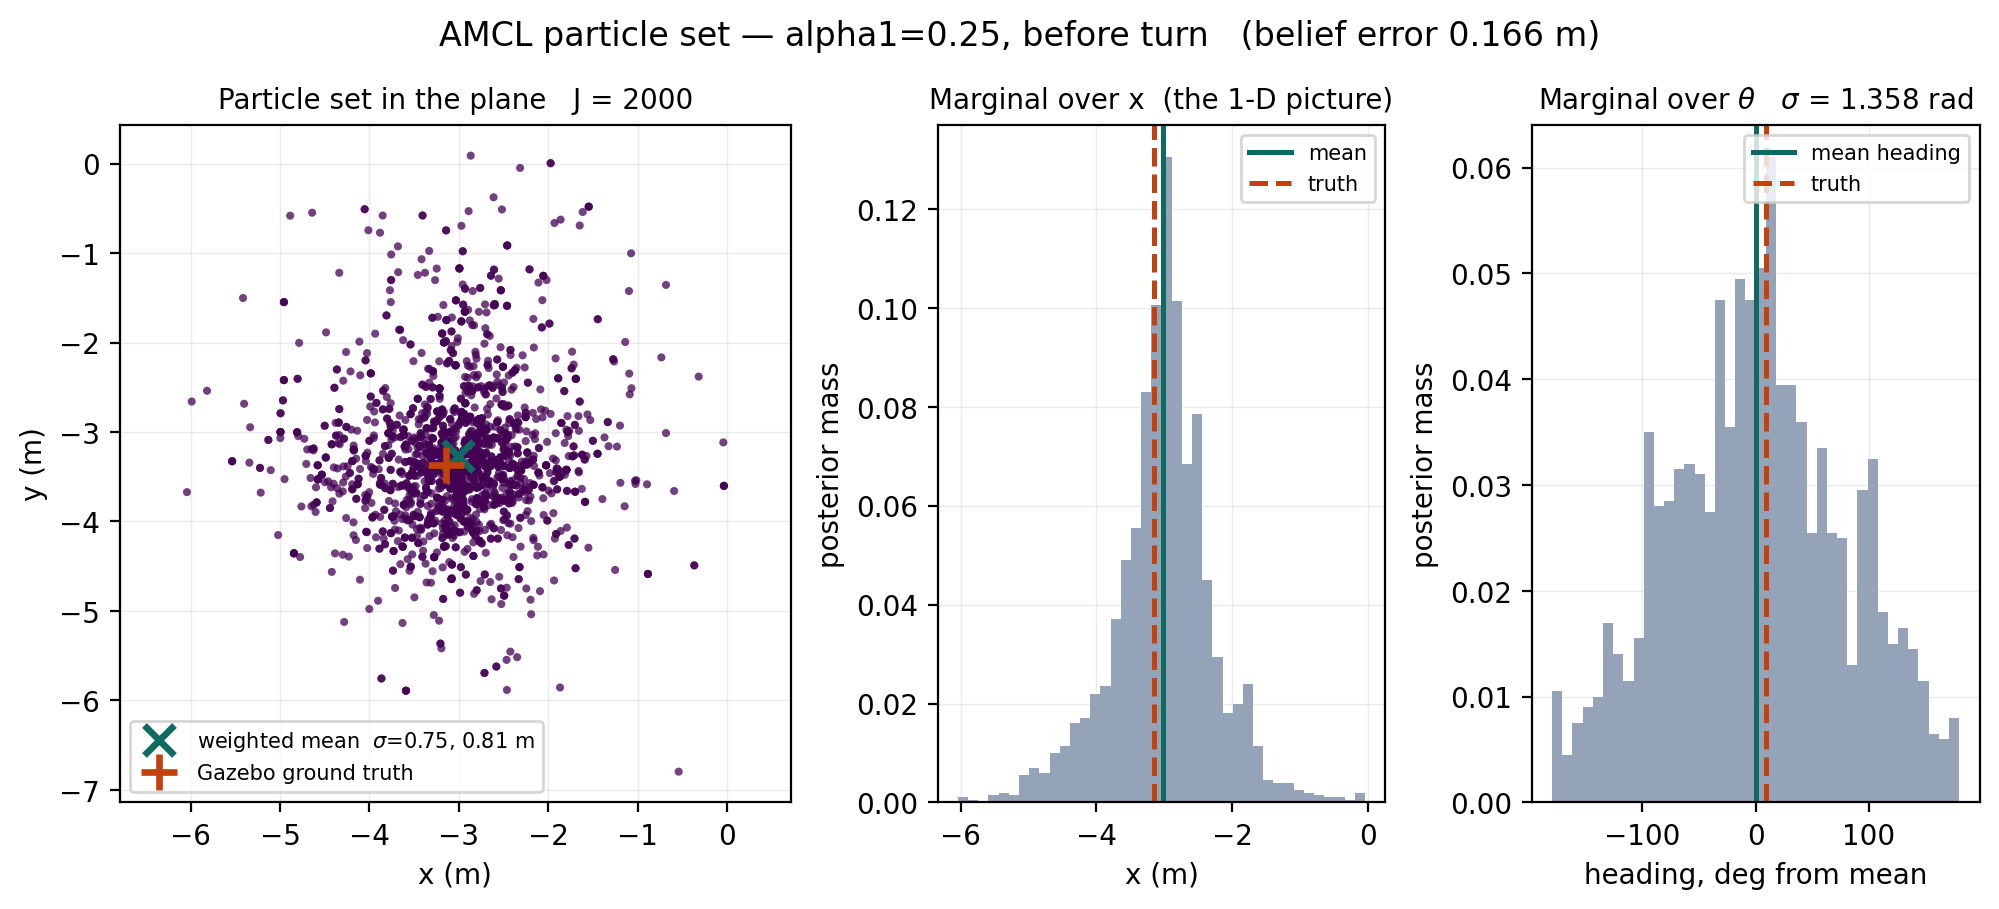
\includegraphics[width=\textwidth]{fig/p3_before.png}\\[2pt]
{\footnotesize (c) before the turn, $\alpha_1 = 0.25$}
\end{minipage}\hfill
\begin{minipage}{0.49\textwidth}\centering
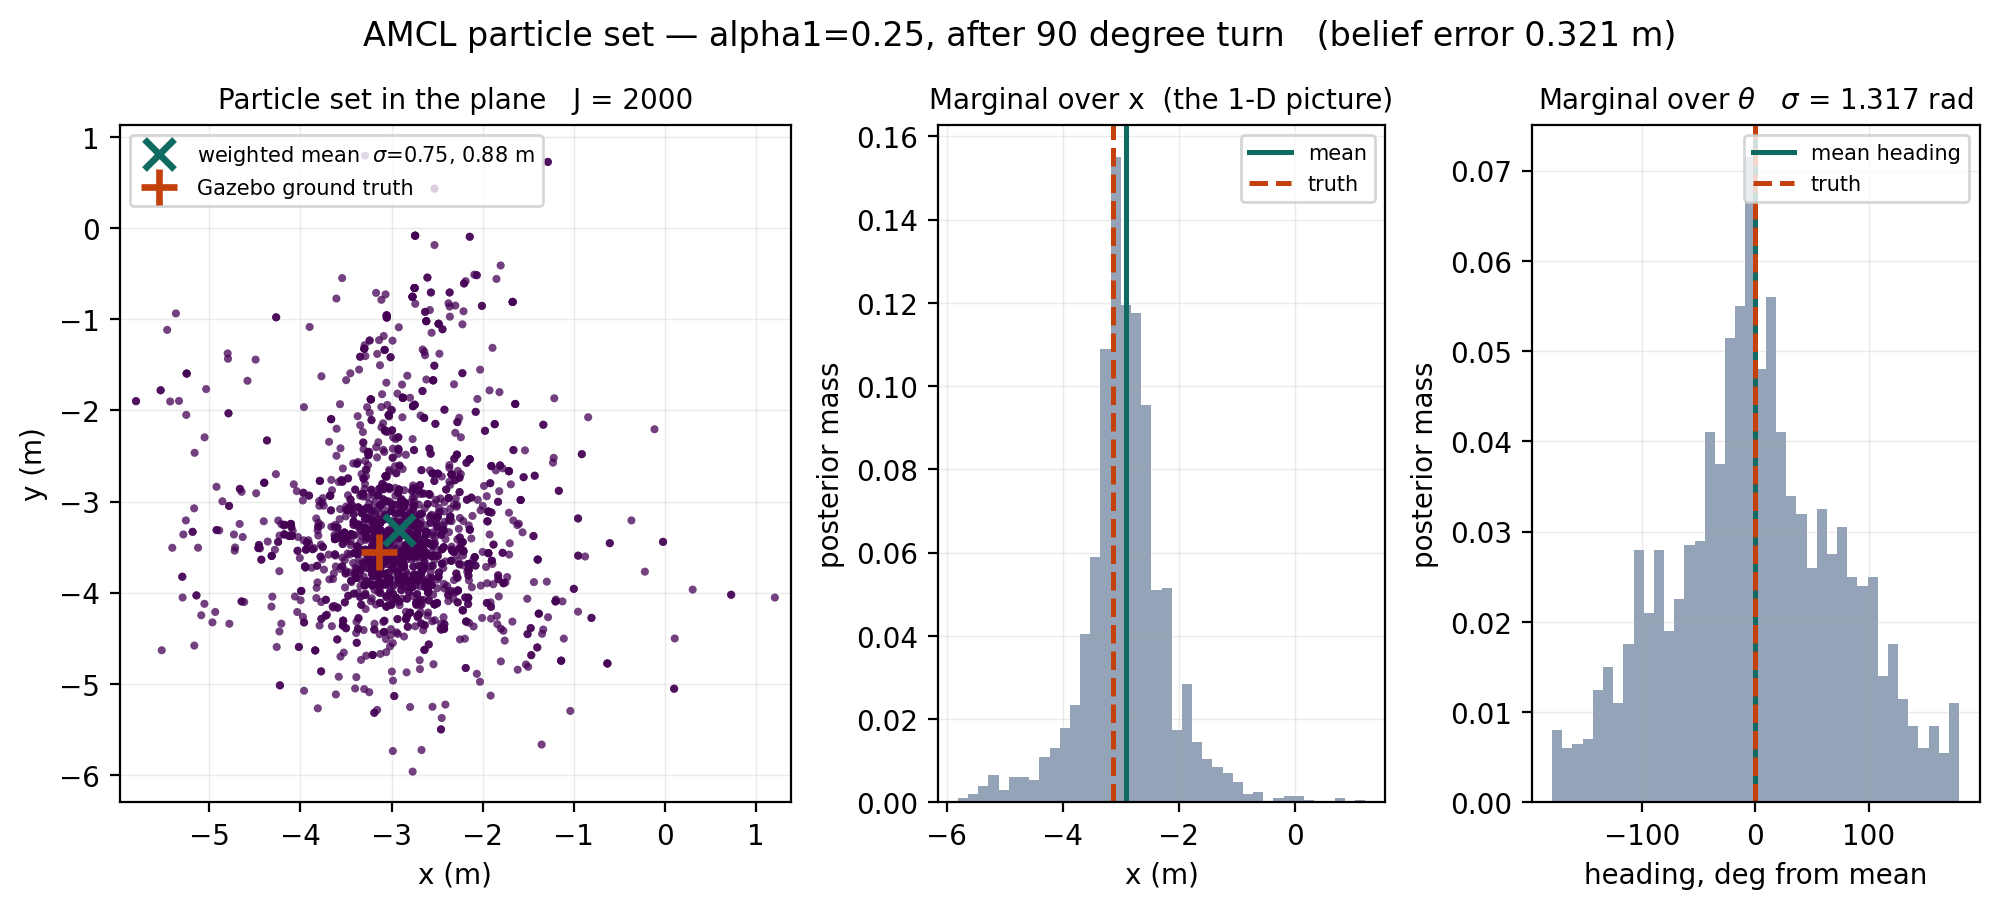
\includegraphics[width=\textwidth]{fig/p4_after.png}\\[2pt]
{\footnotesize (d) after the turn, $\alpha_1 = 0.25$}
\end{minipage}
\caption[Particle cloud, mis-tuned]{The same rotation with the rotational
noise coefficient set to $0.25$. The prediction step sprays particles across a
wide arc, faster than one scan update can pull them back. Panels (c)--(d) are
the visual form of the sweep in Part~5 \S5.3.}
\label{fig:cloud-bad}
\end{figure}

% =========================================================================
\chapter{Resampling: the wheel, and the better wheel}
\label{ch:resample}

Step~3 of the filter said ``draw $J$ new particles, choosing particle $j$ with
probability $w^{[j]}$''. That sentence hides a choice of algorithm, and the two
main candidates behave very differently. This part explains both, works each
one by hand on the same five particles, proves the guarantee that separates
them, and then establishes --- from the actual source code of the software
this project runs --- which one is in use here and why.

\section{The cumulative distribution: turning weights into a ruler}

Both algorithms start the same way. Lay the weights end to end along a line of
total length $1$. Particle $j$ occupies a segment of length $w^{[j]}$. Formally
we build the \term{cumulative distribution} $c$:
\begin{equation}
c_0 = 0, \qquad c_i \;=\; \sum_{j=1}^{i} w^{[j]}
\quad\text{for } i = 1,\ldots,J, \qquad c_J = 1 .
\label{eq:cdf}
\end{equation}

Now ``choosing particle $j$ with probability $w^{[j]}$'' becomes something
mechanical: pick a number $r$ somewhere in $[0,1)$, find which segment it lands
in --- the $i$ with $c_{i-1} \le r < c_i$ --- and take that particle. Because
segment $i$ has length $w^{[i]}$, a uniformly random $r$ lands in it with
probability exactly $w^{[i]}$. That is the requirement, met exactly.

\begin{plain}[Our running example]
Five particles with these weights (they sum to $1$):
\begin{center}
\begin{tabular}{@{}lccccc@{}}
\toprule
particle $j$ & 1 & 2 & 3 & 4 & 5 \\
weight $w^{[j]}$ & 0.05 & 0.35 & 0.10 & 0.42 & 0.08 \\
\midrule
segment & $[0,0.05)$ & $[0.05,0.40)$ & $[0.40,0.50)$ & $[0.50,0.92)$ & $[0.92,1.00)$ \\
\bottomrule
\end{tabular}
\end{center}
Cumulative distribution:
$c = (0,\; 0.05,\; 0.40,\; 0.50,\; 0.92,\; 1.00)$.

\smallskip
With $J = 5$, the number of copies we \emph{ought} to get of each particle is
$J w^{[j]}$:
\[
(0.25,\; 1.75,\; 0.50,\; 2.10,\; 0.40).
\]
Since we can only take whole particles, no algorithm can hit these exactly.
The question is how badly each one misses.
\end{plain}

\section{Method A --- the roulette wheel (multinomial resampling)}

Bend the line of segments into a circle and fit a single pointer. Spin the
pointer $J$ times, independently, and take whichever particle it lands on each
time.

\begin{plain}[Algorithm A: roulette wheel / multinomial]
\begin{enumerate}[leftmargin=1.8em,itemsep=1pt]
\item Build $c$ by equation~\eqref{eq:cdf}.
\item Repeat $J$ times:
  \begin{enumerate}[leftmargin=1.4em,label=\alph*.]
  \item Draw $r \sim \mathrm{Uniform}[0,1)$ --- a \emph{fresh} random number
  every time.
  \item Find $i$ such that $c_{i-1} \le r < c_i$.
  \item Copy particle $i$ into the new set.
  \end{enumerate}
\end{enumerate}
\end{plain}

\begin{handbox}[Method A worked by hand]
Take these five random numbers (any five would do):
$r = 0.13,\; 0.68,\; 0.91,\; 0.07,\; 0.55$.

\begin{center}
\begin{tabular}{@{}cll@{}}
\toprule
$r$ & lands in segment & selects \\
\midrule
0.13 & $[0.05, 0.40)$ & particle 2 \\
0.68 & $[0.50, 0.92)$ & particle 4 \\
0.91 & $[0.50, 0.92)$ & particle 4 \\
0.07 & $[0.05, 0.40)$ & particle 2 \\
0.55 & $[0.50, 0.92)$ & particle 4 \\
\bottomrule
\end{tabular}
\end{center}

\textbf{Result:} counts $(0,\,2,\,0,\,3,\,0)$ against the ideal
$(0.25,\,1.75,\,0.50,\,2.10,\,0.40)$.

Particle 3 carried $10\%$ of the belief and was wiped out. Particle 5 carried
$8\%$ and was wiped out. Nothing went wrong --- this is a perfectly valid draw
--- but a tenth of the filter's information vanished on this one step.
\end{handbox}

\subsection{How much does it miss by? (exact answer)}

Because each of the $J$ draws is independent and each hits particle $j$ with
probability $w^{[j]}$, the count $N_j$ of copies of particle $j$ is a
\term{binomial} random variable:
\begin{equation}
N_j \sim \mathrm{Binomial}\bigl(J,\, w^{[j]}\bigr), \qquad
\mathbb{E}[N_j] = J w^{[j]}, \qquad
\mathrm{Var}[N_j] = J\, w^{[j]}\bigl(1 - w^{[j]}\bigr).
\label{eq:multivar}
\end{equation}
The mean is right --- the method is \emph{unbiased} --- but the variance grows
with $J$. This is the flaw.

\section{Method B --- stochastic universal sampling (systematic, low variance)}

Keep the same wheel. Replace the single pointer with a \emph{comb} of $J$
pointers, rigidly spaced exactly $1/J$ apart. Spin the comb \emph{once}, and
read off all $J$ pointers together.

\begin{plain}[Algorithm B: stochastic universal sampling]
\begin{enumerate}[leftmargin=1.8em,itemsep=1pt]
\item Build $c$ by equation~\eqref{eq:cdf}.
\item Draw \emph{one} random offset $u \sim \mathrm{Uniform}\bigl[0,\; 1/J\bigr)$.
\item For $n = 0, 1, \ldots, J-1$: set the pointer
      $\;r_n = u + \dfrac{n}{J}\;$ and select the particle whose segment
      contains $r_n$.
\end{enumerate}
Only one random number is drawn for the entire step.
\end{plain}

\begin{handbox}[Method B worked by hand, same particles]
$J = 5$, so pointers are spaced $1/5 = 0.20$ apart. Draw one offset
$u = 0.13$ (it must lie in $[0, 0.20)$). The comb is then
\[
r_0 = 0.13,\quad r_1 = 0.33,\quad r_2 = 0.53,\quad r_3 = 0.73,\quad r_4 = 0.93 .
\]

\begin{center}
\begin{tabular}{@{}cll@{}}
\toprule
pointer & lands in segment & selects \\
\midrule
0.13 & $[0.05, 0.40)$ & particle 2 \\
0.33 & $[0.05, 0.40)$ & particle 2 \\
0.53 & $[0.50, 0.92)$ & particle 4 \\
0.73 & $[0.50, 0.92)$ & particle 4 \\
0.93 & $[0.92, 1.00)$ & particle 5 \\
\bottomrule
\end{tabular}
\end{center}

\textbf{Result:} counts $(0,\,2,\,0,\,2,\,1)$ against the ideal
$(0.25,\,1.75,\,0.50,\,2.10,\,0.40)$.

Compare with Method A's $(0,\,2,\,0,\,3,\,0)$. Method B kept particle 5;
Method A did not. And notice that particle 4, whose ideal count is $2.10$,
received exactly $2$ --- it could only ever have received $2$ or $3$, never
$0$ and never $5$.
\end{handbox}

\begin{figure}[htbp]
\centering
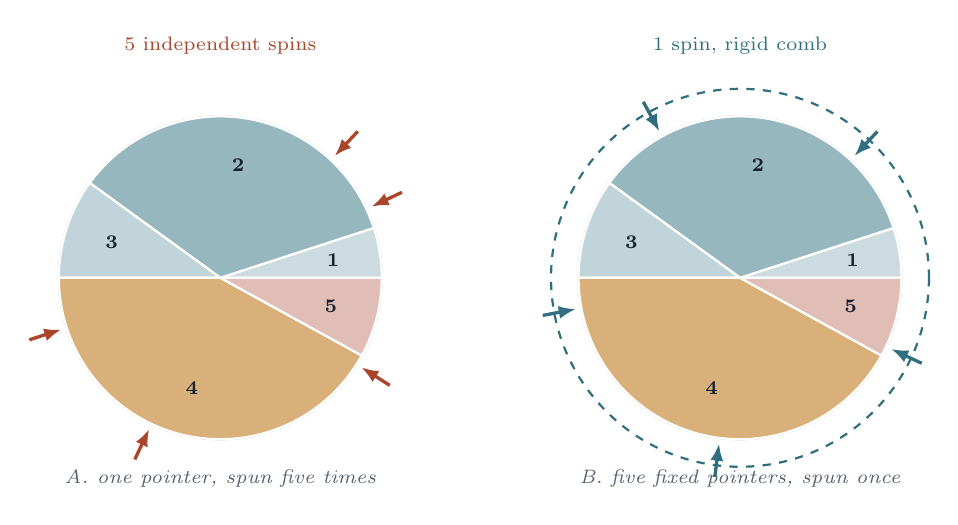
\begin{tikzpicture}[font=\small]
% --- helper: draw a weight wheel -------------------------------------
\def\wheel#1#2{%
  \begin{scope}[shift={(#1,0)}]
  \draw[fill=teal!6,draw=rule,thick] (0,0) circle (2.05);
  % segments: cumulative in fractions of 360
  \foreach \a/\b/\lab/\col in {0/18/1/teal!25, 18/144/2/teal!50, 144/180/3/teal!30,
                               180/331.2/4/amber!60, 331.2/360/5/rust!35} {
    \fill[\col,draw=white,thick] (0,0) -- (\a:2.05) arc (\a:\b:2.05) -- cycle;
  }
  \foreach \m/\lab in {9/1, 81/2, 162/3, 255.6/4, 345.6/5} {
    \node[font=\scriptsize\bfseries,color=ink] at (\m:1.45) {\lab};
  }
  \node[font=\scriptsize\itshape,color=slate] at (0,-2.55) {#2};
  \end{scope}}
\wheel{0}{A. one pointer, spun five times}
\wheel{6.6}{B. five fixed pointers, spun once}
% pointers for A: r = 0.13,0.68,0.91,0.07,0.55 -> angles = r*360
\foreach \r in {46.8, 244.8, 327.6, 25.2, 198} {
  \draw[-{Latex[length=2.2mm]},rust,very thick] (\r:2.55) -- (\r:2.12);
}
\node[font=\scriptsize,color=rust] at (0,2.95) {5 independent spins};
\begin{scope}[shift={(6.6,0)}]
\foreach \r in {46.8, 118.8, 190.8, 262.8, 334.8} {
  \draw[-{Latex[length=2.2mm]},teal,very thick] (\r:2.55) -- (\r:2.12);
}
\draw[teal,thick,dashed] (0,0) circle (2.4);
\node[font=\scriptsize,color=teal] at (0,2.95) {1 spin, rigid comb};
\end{scope}
\end{tikzpicture}
\caption[Two resamplers]{The same weighted wheel, two ways of reading it.
Segment sizes are the weights $(0.05,\,0.35,\,0.10,\,0.42,\,0.08)$. Left: the
roulette wheel is spun five times independently; the pointers clump, and
segments 3 and 5 are missed entirely. Right: five pointers rigidly spaced
$1/5$ of a turn apart are placed by a single spin; they cannot clump, so any
segment wider than $1/5$ of the wheel is certain to be hit.}
\label{fig:wheels}
\end{figure}

\subsection{The guarantee, proved}

\begin{keyidea}[Survival guarantee of stochastic universal sampling]
Under Method B, \emph{every particle whose weight satisfies
$w^{[j]} \ge 1/J$ is selected at least once, with certainty.}
\end{keyidea}

\noindent\textbf{Proof.} Particle $j$ occupies the half-open interval
$[c_{j-1},\, c_j)$ of length $w^{[j]}$. The pointers form the arithmetic
sequence $u,\, u + 1/J,\, u + 2/J,\, \ldots$, and consecutive pointers are
exactly $1/J$ apart. Any interval of length $\ell \ge 1/J$ placed anywhere on
$[0,1)$ must contain at least one point of a lattice of spacing $1/J$: if it
contained none, there would be a gap of length greater than $1/J$ between two
consecutive lattice points, contradicting the spacing. Hence
$w^{[j]} \ge 1/J$ implies at least one pointer lands in particle $j$'s
segment. $\qquad\blacksquare$

Method A offers no such guarantee. Under Method A the probability that
particle $j$ is missed entirely is
\[
P(N_j = 0) = \bigl(1 - w^{[j]}\bigr)^{J},
\]
which is small for large $J$ but never zero.

\subsection{The variance, quantified}

Under Method B the count $N_j$ can only take one of two adjacent whole
numbers. Write $J w^{[j]} = \lfloor J w^{[j]} \rfloor + f_j$, where $f_j$ is
the fractional part. Then
\begin{equation}
N_j \in \bigl\{\lfloor J w^{[j]} \rfloor,\; \lceil J w^{[j]} \rceil \bigr\},
\qquad
\mathbb{E}[N_j] = J w^{[j]},
\qquad
\mathrm{Var}[N_j] = f_j\,(1 - f_j) \;\le\; \tfrac{1}{4}.
\label{eq:susvar}
\end{equation}

The variance is bounded by $1/4$ \emph{regardless of $J$}. Compare with
equation~\eqref{eq:multivar}, where the variance grows linearly in $J$.

\begin{handbox}[Putting numbers on the difference]
Particle 4 in our example: $w = 0.42$, $J = 5$, so $Jw = 2.10$ and $f = 0.10$.

\smallskip
\textbf{Method A (multinomial).}
\[
\mathrm{Var}[N_4] = J w (1-w) = 5 \times 0.42 \times 0.58 = 1.218,
\qquad \sigma = \sqrt{1.218} = 1.10 .
\]
So the count typically wanders by about one whole particle either side of
$2.1$.

\smallskip
\textbf{Method B (systematic).}
\[
\mathrm{Var}[N_4] = f(1-f) = 0.10 \times 0.90 = 0.09,
\qquad \sigma = \sqrt{0.09} = 0.30 .
\]

\smallskip
\textbf{Ratio:} $1.218 / 0.09 = 13.5$. Method B has roughly \textbf{thirteen
times less} count variance on this particle.

\smallskip
Now scale up to this project's actual particle count. With $J = 2000$ and a
particle holding $w = 0.001$:
\[
\text{A:}\;\; \mathrm{Var} = 2000 \times 0.001 \times 0.999 = 1.998
\qquad\text{vs.}\qquad
\text{B:}\;\; \mathrm{Var} \le 0.25 .
\]
And the gap widens as $J$ grows, because A's variance is proportional to $J$
and B's is not.
\end{handbox}

\subsection{Running cost}

\begin{center}
\begin{tabular}{@{}lll@{}}
\toprule
\textbf{Method} & \textbf{Random numbers} & \textbf{Search cost for $J$ draws} \\
\midrule
A, linear scan of $c$   & $J$ & $O(J^2)$ worst case \\
A, binary search on $c$ & $J$ & $O(J \log J)$ \\
B, systematic           & $1$ & $O(J)$ --- one sweep, pointers are sorted \\
\bottomrule
\end{tabular}
\end{center}

Method B is cheaper because the pointers arrive in increasing order, so a
single walk through $c$ serves all of them; no search is needed at all.

\section{Which one does this project actually use, and why?}
\label{sec:whichresampler}

\begin{warnbox}[An honest correction to the framing of the question]
This was not a choice made in this thesis. The resampler is inside
\file{nav2\_amcl}, which this project uses as supplied; there is no parameter
that switches it. The defensible statement is therefore not ``we chose A over
B`` but ''\emph{AMCL} uses A, for a documented reason, and that reason interacts
with a parameter this project \emph{did} set.''
\end{warnbox}

The implementation is \file{nav2\_amcl/src/pf/pf.c}, function
\file{pf\_update\_resample}. On the \texttt{humble} branch --- the branch this
project runs --- it builds the cumulative distribution
\begin{center}
\begin{minipage}{0.8\textwidth}
\begin{plain}
\ttfamily\footnotesize
c[0] = 0.0;\\
for (i = 0; i < set\_a->sample\_count; i++) \{\\
\hspace*{1em}c[i + 1] = c[i] + set\_a->samples[i].weight;\\
\}
\end{plain}
\end{minipage}
\end{center}
and then, for each new particle, draws a fresh random number and scans for its
segment:
\begin{center}
\begin{minipage}{0.8\textwidth}
\begin{plain}
\ttfamily\footnotesize
double r;\\
r = drand48();\\
for (i = 0; i < set\_a->sample\_count; i++) \{\\
\hspace*{1em}if ((c[i] <= r) \&\& (r < c[i + 1])) \{\\
\hspace*{2em}break;\\
\hspace*{1em}\}\\
\}
\end{plain}
\end{minipage}
\end{center}

That is Method A exactly: one independent \file{drand48()} per particle, and a
linear scan rather than a binary search.

The same file contains a commented-out low-variance sampler and the reason it
was not used:

\begin{center}
\begin{minipage}{0.85\textwidth}
\begin{keyidea}[Verbatim comment in \file{nav2\_amcl/src/pf/pf.c}]
\itshape ``Can't (easily) combine low-variance sampler with KLD adaptive
sampling, so we'll take the more traditional route.''
\end{keyidea}
\end{minipage}
\end{center}

\subsection{What KLD adaptive sampling is, and why it blocks Method B}

The ``A'' in AMCL stands for \term{adaptive}, and what adapts is $J$ itself.
Rather than always carrying a fixed number of particles, AMCL carries as few
as it can get away with: many when it is lost and the belief is spread over the
whole building, few when it has converged onto one spot.

The rule it uses is \term{KLD sampling}. The filter drops particles into a
$k$-d tree and counts $k$, the number of distinct occupied bins --- a proxy
for how spread out the belief is. It then computes the number of particles $n$
needed so that the error between the particle approximation and the true
distribution, measured as a Kullback--Leibler divergence, exceeds $\varepsilon$
with probability at most $\delta$:
\begin{equation}
n \;=\; \left\lceil\;
\frac{k-1}{2\varepsilon}
\left(
1 \;-\; \frac{2}{9(k-1)} \;+\; \sqrt{\frac{2}{9(k-1)}}\; z_{1-\delta}
\right)^{\!3}
\;\right\rceil ,
\label{eq:kld}
\end{equation}
then clamps $n$ into $[\,\file{min\_particles},\, \file{max\_particles}\,]$.

The terms:
\begin{itemize}[leftmargin=1.4em,itemsep=2pt]
\item $k$ --- occupied bins in the $k$-d tree. Small $k$ = converged belief.
\item $\varepsilon$ --- the tolerated KL error. In nav2's source,
\file{pf->pop\_err = 0.01}.
\item $z_{1-\delta}$ --- the Gaussian quantile from Part~1 \S1.4. In nav2's
source, \file{pf->pop\_z = 3}, i.e. the ``three sigma'' level, $\delta \approx
0.001$.
\item $\lceil\;\rceil$ --- round up to a whole number of particles.
\end{itemize}

\begin{handbox}[Equation~\eqref{eq:kld} by hand, with this project's limits]
This project sets \file{min\_particles: 500} and \file{max\_particles: 2000}.
Take $k = 5$ occupied bins (a fairly converged cloud).

\smallskip
\textbf{Step 1.} $k - 1 = 4$, so $9(k-1) = 36$.
\[
\frac{2}{9(k-1)} = \frac{2}{36} = 0.055556 .
\]
\textbf{Step 2.} $\sqrt{0.055556} = 0.235702$, and multiplying by $z = 3$:
\[
0.235702 \times 3 = 0.707107 .
\]
\textbf{Step 3.} The bracket:
\[
1 - 0.055556 + 0.707107 = 1.651551 .
\]
\textbf{Step 4.} Cube it:
\[
1.651551^{3} = 4.5048 .
\]
\textbf{Step 5.} Multiply by $\dfrac{k-1}{2\varepsilon} = \dfrac{4}{0.02} = 200$:
\[
200 \times 4.5048 = 900.96 \;\longrightarrow\; \lceil 900.96 \rceil = 901 .
\]
\textbf{Step 6.} Clamp to $[500, 2000]$: $n = \mathbf{901}$ particles.

\medskip
Repeat for $k = 2$ (a very tight cloud):
$2/9 = 0.222222$; $\sqrt{0.222222}\times 3 = 1.414214$;
bracket $= 1 - 0.222222 + 1.414214 = 2.191992$; cubed $= 10.5321$;
$\times\, 1/0.02 = 50$ gives $526.6 \rightarrow 527$. Clamped: $\mathbf{527}$.

\medskip
And $k = 20$ (a badly spread cloud):
$2/171 = 0.011696$; $\sqrt{\cdot}\times 3 = 0.324443$; bracket $= 1.312747$;
cubed $= 2.2623$; $\times\, 19/0.02 = 950$ gives $2149.2 \rightarrow 2150$,
which exceeds \file{max\_particles} and is clamped to $\mathbf{2000}$.

\medskip
So in this project the filter runs between $527$ and $2000$ particles
depending on how uncertain it is --- and the floor of $500$ almost never binds,
because $k = 2$ already asks for $527$.
\end{handbox}

\subsection{The actual incompatibility}

Method B needs to know $J$ \emph{before} it starts, because the pointer
spacing is $1/J$ and the offset must be drawn from $[0, 1/J)$. But KLD
sampling decides $J$ \emph{while} resampling is in progress: nav2 draws
particles one at a time, inserts each into the $k$-d tree, recomputes the
limit from equation~\eqref{eq:kld}, and stops when it has enough:
\begin{center}
\begin{minipage}{0.8\textwidth}
\begin{plain}
\ttfamily\footnotesize
if (set\_b->sample\_count > pf\_resample\_limit(pf, set\_b->kdtree->leaf\_count)) \{\\
\hspace*{1em}break;\\
\}
\end{plain}
\end{minipage}
\end{center}
The target count is a moving quantity that depends on the particles drawn so
far. A rigid comb of $1/J$-spaced pointers cannot be laid down against a $J$
that is not yet known. That is the incompatibility the source comment refers
to, stated concretely.

\subsection{What this means for this project's results}

\begin{plain}[The defensible position]
\begin{enumerate}[leftmargin=1.6em,itemsep=3pt]
\item AMCL uses multinomial (roulette-wheel) resampling. This is verifiable in
\file{nav2\_amcl/src/pf/pf.c} and is not configurable.
\item It does so in order to keep KLD adaptive sampling, which this project
relies on --- \file{min\_particles: 500}, \file{max\_particles: 2000} are
meaningless without it.
\item The price is higher count variance and no survival guarantee, so
\term{particle depletion} is bounded only probabilistically, not absolutely.
\item This project sets \file{resample\_interval: 1} --- resample on every
update --- which is the setting that most exposes that price. Raising it is a
tuning lever, listed in Part~11.
\item The mitigation actually used here was not to change the resampler but to
\emph{reduce the need for it}: sharpening the measurement likelihood
(\file{z\_hit} $0.5 \rightarrow 0.8$, \file{laser\_max\_range}
$8 \rightarrow \SI{16}{\metre}$, \file{max\_beams} $60 \rightarrow 120$) so
that weights are informative, and narrowing the motion model
($\alpha_1 = \alpha_2 : 0.25 \rightarrow 0.02$) so that fewer particles are
thrown into low-weight regions in the first place. Both are covered in Part~5.
\end{enumerate}
\end{plain}

% =========================================================================
\chapter{AMCL: every knob, and what it does}
\label{ch:amcl}

\term{AMCL} stands for \emph{Adaptive Monte Carlo Localisation}. Taking the
words backwards: \emph{Localisation} --- working out where the robot is;
\emph{Monte Carlo} --- doing it with the crowd of particles from Part~3;
\emph{Adaptive} --- varying the size of the crowd by the KLD rule of
Part~4~\S4.4.

This part goes through the configuration used in this project,
\file{config/nav2\_params.yaml}, and says what each parameter physically does.
It is organised by the split that matters --- proposal versus weight.

\section{The split: what you choose, and what chooses you}

Return to importance sampling, equation~\eqref{eq:importance}. There are
exactly two ingredients: the proposal $\pi$ you sample from, and the weight
$w = p/\pi$ you correct with. They are not symmetric.

\begin{keyidea}[The proposal is a design choice; the weight is not]
$\pi$ is \emph{yours}. Any $\pi$ satisfying the support
condition~\eqref{eq:support} gives a correct estimator; a bad $\pi$ makes it
\emph{inefficient}, needing more particles for the same accuracy, but it still
converges on the right answer.

$w$ is \emph{forced}. Once you have chosen $\pi$, the weight must be $p/\pi$
exactly. Get it wrong and the ratio no longer cancels in
equation~\eqref{eq:importance}: you are now computing an average under some
other density altogether. A weight fault does not make the estimator slow ---
it makes it answer a different question, confidently.
\end{keyidea}

In AMCL:
\begin{itemize}[leftmargin=1.4em,itemsep=2pt]
\item the \textbf{proposal} is the \term{motion model}, governed by
$\alpha_1 \ldots \alpha_5$;
\item the \textbf{weight} is the \term{measurement model}, governed by
\file{z\_hit}, \file{z\_rand}, \file{z\_short}, \file{z\_max},
\file{sigma\_hit}, \file{max\_beams} and\linebreak \file{laser\_max\_range}.
\end{itemize}

\begin{plain}[Answering the question directly: what did this project choose?]
This project chose the \textbf{proposal}. Specifically it chose
$\alpha_1 = \alpha_2 = 0.02$ and $\alpha_3 = \alpha_4 = \alpha_5 = 0.05$, by
sweeping and measuring rather than by reasoning (\S5.3), and it chose to
disable divergence recovery, $\file{recovery\_alpha\_slow} =
\file{recovery\_alpha\_fast} = 0$ (\S5.5).

It also \textbf{corrected the weight} --- but that is a different kind of act.
The scanner fitted to ROMR reaches \SI{16}{\metre} and
\file{laser\_max\_range} was set to \SI{8}{\metre}. That is not a preference;
it is a description of the sensor that was factually false, and it was
therefore a \emph{fault}, not a tuning. Correcting it to \SI{16}{\metre}
restored the correspondence between $w$ and $p/\pi$. The same applies to
raising \file{z\_hit} from $0.5$ to $0.8$: the value $0.5$ asserted that half
of every scan is meaningless noise, and the measurement in \S5.4 shows that
against this map it is not.
\end{plain}

\section{The proposal: the odometry motion model and the five alphas}

At each step, AMCL takes the change in odometry and decomposes it into three
elementary movements: an initial rotation, a translation, and a final
rotation.

\begin{figure}[htbp]
\centering
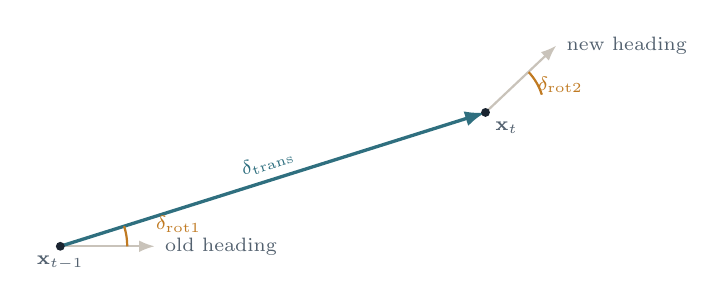
\begin{tikzpicture}[font=\small,scale=1.0]
\coordinate (A) at (0,0);
\coordinate (B) at (5.4,1.7);
\draw[rule,thick,-{Latex[length=2mm]}] (A) -- ++(1.2,0) node[right,font=\scriptsize,color=slate] {old heading};
\draw[teal,very thick,-{Latex[length=2.6mm]}] (A) -- (B);
\draw[rule,thick,-{Latex[length=2mm]}] (B) -- ++(0.9,0.85) node[right,font=\scriptsize,color=slate] {new heading};
\draw[amber,thick] (0.85,0) arc (0:17.5:0.85);
\node[amber,font=\scriptsize] at (1.5,0.28) {$\delta_{\text{rot}1}$};
\node[teal,font=\scriptsize,above,rotate=17.5] at (2.7,0.85) {$\delta_{\text{trans}}$};
\draw[amber,thick] ($(B)+(17.5:0.75)$) arc (17.5:43:0.75);
\node[amber,font=\scriptsize] at (6.35,2.05) {$\delta_{\text{rot}2}$};
\fill[ink] (A) circle (1.6pt); \fill[ink] (B) circle (1.6pt);
\node[below,font=\scriptsize,color=slate] at (A) {$\xt_{t-1}$};
\node[below right,font=\scriptsize,color=slate] at (B) {$\xt_{t}$};
\end{tikzpicture}
\caption[Odometry decomposition]{Any change of pose is written as: turn on the
spot to face the destination ($\delta_{\text{rot}1}$), drive straight
($\delta_{\text{trans}}$), turn on the spot to the final heading
($\delta_{\text{rot}2}$). The five $\alpha$ coefficients say how much random
error to add to each of these three, and where that error comes from.}
\label{fig:odomdecomp}
\end{figure}

The decomposition is
\begin{equation}
\begin{aligned}
\delta_{\text{rot}1} &= \operatorname{atan2}(\bar{y}' - \bar{y},\; \bar{x}' - \bar{x}) - \bar\theta, \\
\delta_{\text{trans}} &= \sqrt{(\bar{x}' - \bar{x})^2 + (\bar{y}' - \bar{y})^2}, \\
\delta_{\text{rot}2} &= \bar\theta' - \bar\theta - \delta_{\text{rot}1},
\end{aligned}
\label{eq:odomdelta}
\end{equation}
where barred quantities are what the \emph{odometry} reports (not the truth).

AMCL then perturbs each of the three with zero-mean noise whose variance is
built from the alphas:
\begin{equation}
\begin{aligned}
\hat\delta_{\text{rot}1} &= \delta_{\text{rot}1}
   - \mathcal{E}\bigl(\alpha_1 \delta_{\text{rot}1}^2 + \alpha_2 \delta_{\text{trans}}^2\bigr), \\
\hat\delta_{\text{trans}} &= \delta_{\text{trans}}
   - \mathcal{E}\bigl(\alpha_3 \delta_{\text{trans}}^2 + \alpha_4 (\delta_{\text{rot}1}^2 + \delta_{\text{rot}2}^2)\bigr), \\
\hat\delta_{\text{rot}2} &= \delta_{\text{rot}2}
   - \mathcal{E}\bigl(\alpha_1 \delta_{\text{rot}2}^2 + \alpha_2 \delta_{\text{trans}}^2\bigr),
\end{aligned}
\label{eq:alphas}
\end{equation}
where $\mathcal{E}(b)$ means ``a random draw with mean zero and variance $b$''.
Each particle gets its own independent draw, which is what makes the cloud
spread.

\begin{center}
\begin{tabular}{@{}llp{7.6cm}@{}}
\toprule
\textbf{Parameter} & \textbf{This project} & \textbf{What it means} \\
\midrule
$\alpha_1$ & 0.02 & rotational error caused by rotating \\
$\alpha_2$ & 0.02 & rotational error caused by translating \\
$\alpha_3$ & 0.05 & translational error caused by translating \\
$\alpha_4$ & 0.05 & translational error caused by rotating \\
$\alpha_5$ & 0.05 & extra term used by omnidirectional models; inert for a
                    differential-drive robot \\
\bottomrule
\end{tabular}
\end{center}

\begin{keyidea}[Read the units carefully --- this is where the mistake was made]
Look at equation~\eqref{eq:alphas}. The alphas multiply the \emph{square of the
motion}, and the result is a \emph{variance}. So $\alpha_1$ is not ``how much I
distrust rotation'' on some abstract scale. It is the constant of
proportionality between the size of a turn and the variance of the error
attributed to that turn. Doubling $\alpha_1$ doubles the variance, which
multiplies the standard deviation --- the physical spread of the cloud --- by
$\sqrt{2}$.
\end{keyidea}

\section{The tuning that went backwards, and what it teaches}
\label{sec:alphasweep}

ROMR's casters are fixed and scrub \SI{180}{}--\SI{220}{\milli\metre} per
turn. The obvious inference: rotational odometry is unreliable, therefore
$\alpha_1$ should be \emph{raised} so the filter trusts it less. That was
tried, at $\alpha_1 = 0.25$. It is the worst setting on the curve.

Sweeping $\alpha_1 = \alpha_2$, re-seeding from ground truth before each
trial, and applying one \ang{90} turn:

\begin{center}
\begin{tabular}{@{}cccc@{}}
\toprule
$\alpha_1 = \alpha_2$ & $e$ (\si{\metre}) & $\Delta\theta$ (\si{\degree}) & $\sigma_\theta$ (\si{\radian}) \\
\midrule
0.25 & 0.469 & $-13.3$ & 1.257 \\
0.10 & 0.279 & $-9.5$  & 0.958 \\
0.05 & 0.168 & $+1.0$  & 0.694 \\
0.02 & \textbf{0.108} & $-2.8$ & \textbf{0.441} \\
0.01 & 0.104 & $-1.8$  & 0.364 \\
\bottomrule
\end{tabular}
\end{center}

\begin{figure}[htbp]
\centering
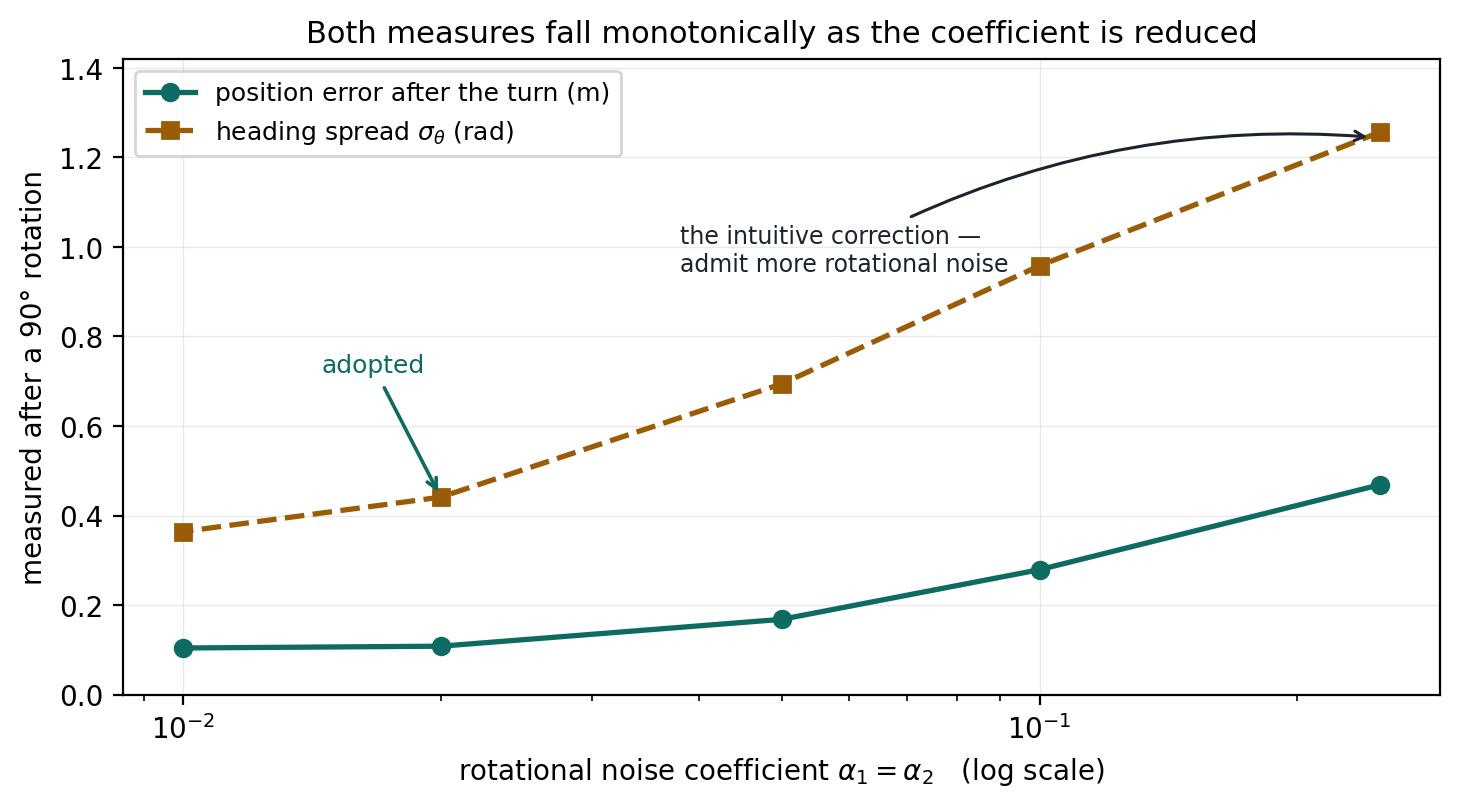
\includegraphics[width=0.92\textwidth]{fig/alpha_sweep.png}
\caption[The alpha sweep]{Position error and heading standard deviation after
a single \ang{90} rotation, against the rotational noise coefficient.
Monotonic and decreasing across the swept range, flattening below $0.02$.
Regenerate with \file{scripts/plot\_results.py}.}
\label{fig:alphasweep}
\end{figure}

\begin{plain}[Why raising $\alpha_1$ made it worse --- the race, again]
Part~2 \S2.4 put it as a race: prediction spreads the belief, correction pulls
it in. Raising $\alpha_1$ makes the prediction step spray particles across a
wide arc. The arc grows faster than one scan update can pull it back, so the
next prediction starts from an already-spread cloud and sprays wider still.
The filter loses the race.

The correct reading of the caster scrub is not ``add noise''. It is: \emph{the
scrub is a systematic error, not a random one}. It biases the odometry the
same way every time. Random noise in the motion model cannot represent a
systematic bias; all it does is degrade the proposal. The systematic part has
to be handled by the measurement, and the measurement can only handle it if it
is sharp enough --- which is what \S5.4 is about.
\end{plain}

Why $0.02$ and not $0.01$, when $0.01$ measured marginally better? Because a
filter that believes its odometry perfectly has no mechanism to accept a
correction when the odometry is finally wrong. The scrub is real. $0.02$ keeps
enough genuine rotational noise in the model to leave the correction step
something to work with, at a cost of \SI{0.004}{\metre} in the measured error.
That is a judgement, and it is stated as one.

\section{The weight: the measurement model}
\label{sec:measmodel}

The laser publishes a scan $\mathbf{z} = \{z_1, \ldots, z_K\}$ of range
readings. For a candidate pose $\xt$ and the map $m$, AMCL scores it by
equation~\eqref{eq:beamproduct}. Each individual beam likelihood is a mixture
of four things that could have produced that reading:

\begin{equation}
p(z_k \mid \xt, m)
= z_{\text{hit}}\, p_{\text{hit}}
+ z_{\text{short}}\, p_{\text{short}}
+ z_{\text{max}}\, p_{\text{max}}
+ z_{\text{rand}}\, p_{\text{rand}},
\qquad \textstyle\sum z_\bullet = 1 .
\label{eq:beammix}
\end{equation}

\begin{center}
\begin{tabular}{@{}llp{7.0cm}@{}}
\toprule
\textbf{Component} & \textbf{This project} & \textbf{What it models} \\
\midrule
$z_{\text{hit}}$   & \textbf{0.80} & the beam hit the wall the map predicts;
   modelled as a Gaussian of width \file{sigma\_hit} around the expected range \\
$z_{\text{short}}$ & 0.05 & the beam hit something not in the map (a person,
   an object); exponential, rate \file{lambda\_short} \\
$z_{\text{max}}$   & 0.05 & the beam hit nothing and returned max range \\
$z_{\text{rand}}$  & \textbf{0.20} & the beam is nonsense; uniform over the range \\
\bottomrule
\end{tabular}
\end{center}

\noindent The dominant term is the first. Writing $\hat{z}_k$ for the range
the map says \emph{ought} to be measured from pose $\xt$ along beam $k$:
\begin{equation}
p_{\text{hit}}(z_k \mid \xt, m)
= \frac{1}{\sqrt{2\pi\,\sigma_{\text{hit}}^{2}}}
  \exp\!\left(-\frac{(z_k - \hat{z}_k)^{2}}{2\,\sigma_{\text{hit}}^{2}}\right),
\label{eq:phit}
\end{equation}
which is exactly the Gaussian of equation~\eqref{eq:gaussian}, centred on the
predicted range. In this project $\sigma_{\text{hit}} = \SI{0.2}{\metre}$: a
beam within \SI{20}{\centi\metre} of where the map says the wall is counts as
a good match.

\begin{warnbox}[Why $z_{\text{hit}}+z_{\text{rand}} = 0.5/0.5$ was wrong here]
Setting $z_{\text{hit}} = z_{\text{rand}} = 0.5$ asserts that half of every
scan is meaningless. Whether that is true is measurable, and it was measured.
Taking a scan at the \emph{true} pose and asking how far each of the $720$
beams falls from the nearest wall in the map:

\begin{center}
\begin{tabular}{@{}lc@{}}
\toprule
Mean distance to nearest wall & \SI{0.047}{\metre} \\
Median distance               & \SI{0.050}{\metre} \\
Within \SI{0.10}{\metre}      & $66.8\%$ \\
Within \SI{0.20}{\metre}      & $100\%$ \\
\bottomrule
\end{tabular}
\end{center}

Every single beam agrees with the map to within \SI{20}{\centi\metre}. In this
environment there is essentially no noise to model. Weighting the informative
term at $0.8$ rather than $0.5$ sharpens the likelihood peak, which is exactly
what wins the race in \S5.3.
\end{warnbox}

\subsection{The other two weight faults}

\textbf{\file{laser\_max\_range}: 8 $\rightarrow$ 16 metres.} The fitted
scanner reaches \SI{16}{\metre}; the building is \SI{13.85}{\metre} across. An
\SI{8}{\metre} cutoff discards exactly the long returns that pin a pose down
along a corridor. A robot in a featureless hallway with only short beams
available has no way to tell where along the hallway it is; the likelihood
becomes flat in one direction, and the belief slides.

\smallskip
\textbf{\file{max\_beams}: 60 $\rightarrow$ 120.} Of the $720$ beams
available, $60$ leaves the likelihood peak shallower than the cost justifies.
$120$ deepens it. Note the tension with the independence caveat of Part~1
\S1.6: more beams means a sharper peak, but also more over-confidence from
treating correlated beams as independent. $120$ of $720$ --- one beam every
\ang{3} --- was the compromise adopted.

\section{Divergence recovery, and why it is off here}

AMCL can inject random particles across the map when it suspects it is lost.
It decides this by comparing a fast-moving and a slow-moving average of the
total particle weight; if the fast average drops well below the slow one, the
scan has stopped matching and something is wrong. The rate constants are
\file{recovery\_alpha\_fast} and \file{recovery\_alpha\_slow}, and the widely
quoted values are $0.1$ and $0.001$.

This project sets both to $\mathbf{0}$, disabling the feature. That is
unusual, and the reasoning is worth spelling out.

\begin{plain}[The argument for switching it off, in three steps]
\textbf{1. It measurably made things worse.} With recovery enabled,
$\sigma_\theta$ reached \SI{2.53}{\radian} --- close to uniform over a full
circle --- while the robot sat \SI{8.5}{\metre} from where AMCL said it was.

\textbf{2. The mechanism is clear.} The pose AMCL publishes is the mean over
\emph{all} particles. Injecting random particles across the map therefore drags
the reported mean away from a cluster that may have been perfectly good.
Recovery does not replace a bad answer with a better one; it dilutes whatever
answer exists.

\textbf{3. The precondition does not hold here.} Recovery earns its place when
the environment is ambiguous --- when a scan is genuinely consistent with two
or more distinct poses, and the filter can back the wrong one. Measured
against this map, that ambiguity does not exist. Rotating the assumed heading
about the true pose and recomputing scan--map agreement gives
\SI{0.047}{\metre} at zero offset, against \SI{0.443}{\metre} at \ang{+45},
\SI{0.410}{\metre} at \ang{+90}, \SI{0.762}{\metre} at \ang{+135} and
\SI{0.749}{\metre} at \ang{180}. There is one sharp global minimum and no
second hypothesis for recovery to find.
\end{plain}

\begin{warnbox}[The cost of this decision, stated plainly]
With recovery off, if localisation is ever genuinely lost, AMCL will
\emph{not} recover on its own. It must be re-seeded --- by
\file{scripts/seed.sh}, or by clicking \textbf{2D Pose Estimate} in RViz. This
is an acceptable trade in a mapped, unambiguous, single-storey environment. It
would not be acceptable in a repetitive one (a hotel corridor, a warehouse
aisle), and a reviewer is entitled to say so.
\end{warnbox}

\section{The remaining parameters}

\begin{center}
\small
\begin{tabular}{@{}llp{7.3cm}@{}}
\toprule
\textbf{Parameter} & \textbf{Value} & \textbf{Meaning} \\
\midrule
\file{min\_particles}  & 500  & floor on $J$ from equation~\eqref{eq:kld} \\
\file{max\_particles}  & 2000 & ceiling on $J$ \\
\file{update\_min\_d}  & \SI{0.25}{\metre} & do not run a filter update until the
   robot has moved this far; saves compute and avoids resampling on noise \\
\file{update\_min\_a}  & \SI{0.2}{\radian} & same, for rotation (\ang{11.5}) \\
\file{resample\_interval} & 1 & resample on \emph{every} update; see Part~11 \\
\file{laser\_min\_range} & \SI{0.15}{\metre} & ignore returns from the robot's own body \\
\file{laser\_max\_range} & \SI{16}{\metre} & matches the fitted scanner \\
\file{sigma\_hit}      & \SI{0.2}{\metre} & width of the Gaussian in eq.~\eqref{eq:phit} \\
\file{lambda\_short}   & 0.1 & decay rate of the unexpected-obstacle term \\
\file{transform\_tolerance} & \SI{1.0}{\second} & how long the published
   \texttt{map}$\rightarrow$\texttt{odom} transform stays valid \\
\file{robot\_model\_type} & \file{DifferentialMotionModel} & selects eq.~\eqref{eq:alphas} \\
\file{tf\_broadcast}   & true & AMCL publishes the correction (Figure~\ref{fig:tf}) \\
\file{set\_initial\_pose} & false & the pose is supplied externally, by RViz or \file{seed.sh} \\
\bottomrule
\end{tabular}
\end{center}

\section{What AMCL reports back, and the covariance}

AMCL publishes on \file{/amcl\_pose}, a
\file{geometry\_msgs/PoseWithCovarianceStamped}. Two things are in it.

\textbf{The pose} is the weighted mean over the particle set --- the Monte
Carlo version of equation~\eqref{eq:expectation}:
\begin{equation}
\hat{\xt} \;=\; \sum_{j=1}^{J} w^{[j]}\, \xt^{[j]} .
\label{eq:posemean}
\end{equation}

\textbf{The covariance} is the spread about that mean:
\begin{equation}
\Sigma \;=\; \sum_{j=1}^{J} w^{[j]}
\bigl(\xt^{[j]} - \hat{\xt}\bigr)\bigl(\xt^{[j]} - \hat{\xt}\bigr)^{\!\top} .
\label{eq:cov}
\end{equation}
$\Sigma$ is a $6 \times 6$ matrix. Its diagonal entries are the variances, and
their square roots are the standard deviations this project logs as
\file{sigma\_x}, \file{sigma\_y} and \file{sigma\_yaw}. The validation script
combines the first two into
\[
\sigma_{\text{pos}} = \sqrt{\sigma_x^2 + \sigma_y^2}.
\]

\begin{warnbox}[The covariance is the filter's opinion of itself]
$\Sigma$ measures how much the \emph{particles} disagree with each other. It
does not measure how far they are from the truth. In the initial run the
particles agreed closely with one another --- small $\sigma$ --- while sitting
\SI{15}{\metre} from the robot. A confident filter and a correct filter are
different things, and the whole evaluation design in Part~7 exists because of
that distinction.
\end{warnbox}

% =========================================================================
\chapter{Nav2: the stack around the filter}
\label{ch:nav2}

\section{What Nav2 is}

\term{Nav2} (Navigation 2) is the ROS~2 navigation stack. You hand it a goal
pose; it plans a route, drives the robot along it, recovers when it gets
stuck, and eventually reports an outcome. It is built as a set of independent
\term{servers}, each doing one job, coordinated by a \term{behaviour tree}.

\begin{figure}[htbp]
\centering
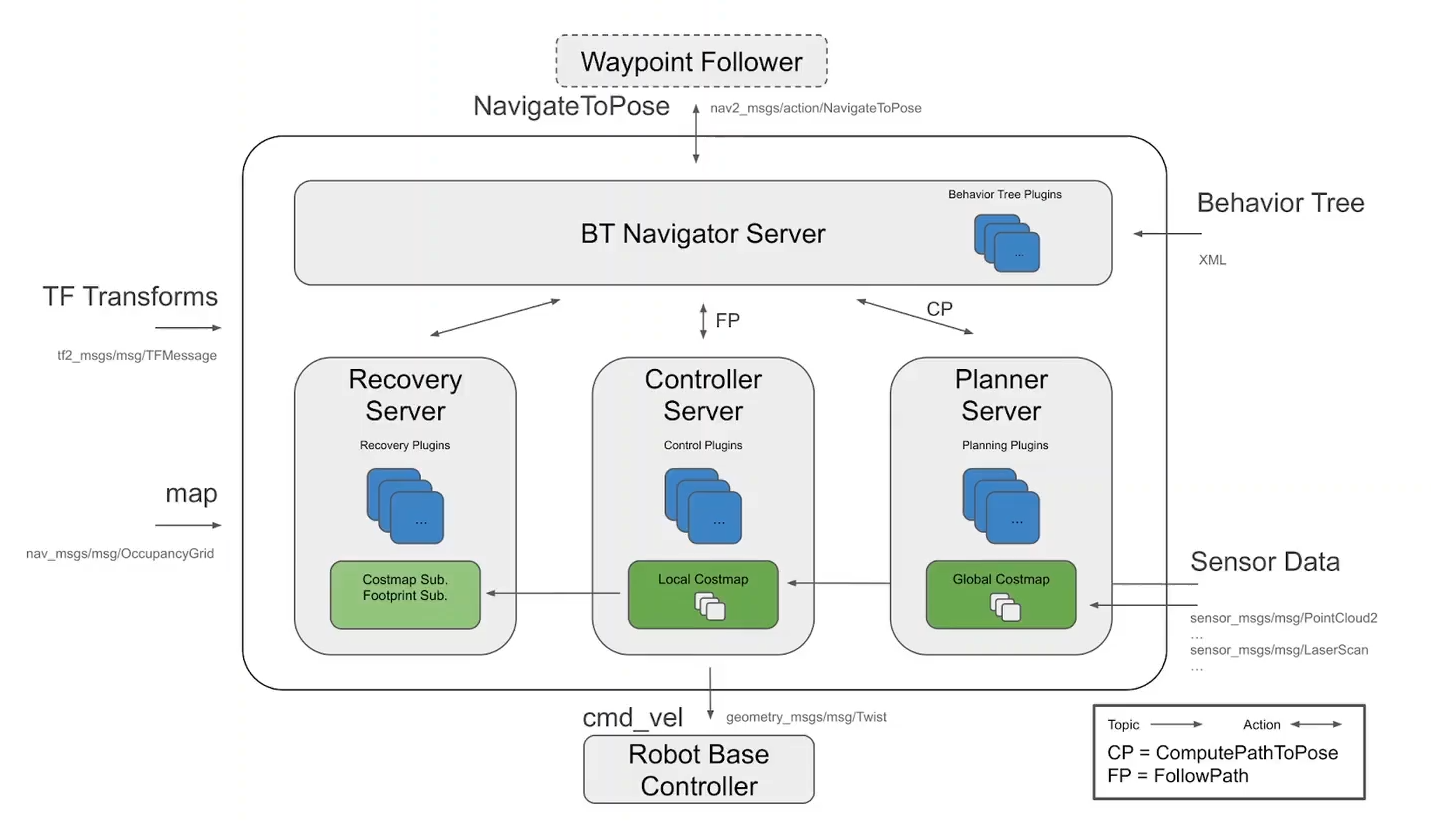
\includegraphics[width=\textwidth]{fig/nav2_arch.png}
\caption[Nav2 architecture]{The Navigation~2 architecture, reproduced from the
Navigation~2 documentation. A goal enters as a \file{NavigateToPose} action at
the BT Navigator Server, which calls the Planner, Controller and Recovery
Servers through further actions (\textbf{CP} = \file{ComputePathToPose},
\textbf{FP} = \file{FollowPath}). The output is a stream of \file{cmd\_vel}
velocity commands to the base controller. Single arrows are topics; double
arrows are actions. \emph{This figure is not original work and should be cited
to its source wherever it is used.}}
\label{fig:nav2arch}
\end{figure}

\subsection{Server by server}

\begin{description}[leftmargin=0pt,style=nextline,font=\bfseries\color{teal}]
\item[BT Navigator Server] The coordinator. It runs a behaviour tree --- an XML
file describing what to try, in what order, and what to do on failure. It
accepts the \file{NavigateToPose} action and is the only server the outside
world talks to.

\item[Planner Server] Given a start and a goal, produces a path. This project
uses \file{NavFn} under the plugin name \file{GridBased}: a grid search over
the global costmap, described in detail in \S\ref{sec:which-planner}. It answers the
\file{ComputePathToPose} (CP) action. When this project logged ``failed to
create plan'', it was this server.

\item[Controller Server] Given a path, produces velocity commands. This project
uses \file{DWBLocalPlanner} (Dynamic Window Approach): at every one of its
\SI{20}{\hertz} cycles it simulates a fan of candidate trajectories
$\SI{1.5}{\second}$ into the future, scores each with a set of
\term{critics} --- \file{PathAlign}, \file{GoalAlign}, \file{BaseObstacle},
\file{RotateToGoal}, \file{Oscillation}, \file{PathDist} --- and issues the
best. It answers the \file{FollowPath} (FP) action. It also hosts the goal
checker and the progress checker, which \S6.4 shows to be the source of this
project's remaining defect.

\item[Recovery Server] What to do when stuck: spin in place, back up, wait,
clear the costmaps. This is the server that produced the sideways shuffling
observed at the garage.

\item[Costmaps] Two occupancy grids. The \term{global costmap} covers the whole
building and is what the planner searches. The \term{local costmap} is a small
rolling window around the robot and is what the controller uses to avoid
things that have just appeared.
\end{description}

\subsection{Which planning algorithm --- and why not RRT}
\label{sec:which-planner}

Path planners split into two families, and it is worth knowing which one you
are using and why.

\textbf{Search-based methods} treat the map as a grid of cells and examine
them systematically. \term{Dijkstra's algorithm} expands outward from the
goal like a flood, one ring of cells at a time, recording for every cell how
far it is from the goal. When the flood reaches the robot, you follow the
numbers downhill and that is your path. \term{A$^{\ast}$} is the same
algorithm with one addition: a \term{heuristic} that guesses how far each
cell still is from the target, so the flood is steered towards the goal
instead of spreading in all directions. Same path, fewer cells examined.

\textbf{Sampling-based methods} do not enumerate anything. \term{RRT}
(Rapidly-exploring Random Tree) throws a random point into the space, finds
the nearest point already on its tree, and grows a short branch towards it,
discarding the branch if it hits an obstacle. Repeat until the tree reaches
the goal. \term{RRT$^{\ast}$} adds a rewiring step: each time a new node is
added, nearby nodes check whether routing through the newcomer would be
cheaper, and reconnect if so. Plain RRT finds \emph{a} path; RRT$^{\ast}$
converges towards the \emph{best} one.

\begin{keyidea}[What this project uses]
From \file{config/nav2\_params.yaml}:
\begin{center}\small
\begin{tabular}{@{}ll@{}}
\toprule
\file{plugin} & \file{nav2\_navfn\_planner/NavfnPlanner} \\
\file{use\_astar} & \file{false} \\
\file{allow\_unknown} & \file{true} \\
\file{tolerance} & \file{0.5} \\
\bottomrule
\end{tabular}
\end{center}
\file{use\_astar: false} means it is \textbf{Dijkstra}, not A$^{\ast}$.
Flipping that one word to \file{true} gives you A$^{\ast}$; on a building
$277 \times 232$ cells across the difference is a few milliseconds, which is
why it was never worth changing.

\textbf{No planner was written for this project.} NavFn is a stock Nav2
plugin. It was configured, not implemented --- and the same is true of the DWB
controller.
\end{keyidea}

\begin{warnbox}[\file{allow\_unknown: true} --- and why it compounds a defect]
This setting permits the planner to route through cells the map records as
unknown. Read \S6.3 on how unknown cells are encoded before deciding whether
that is safe here; the short version is that this project had \emph{two}
independent mechanisms letting paths escape into unmapped space, and only one
of them was a map defect.
\end{warnbox}

\textbf{So why no RRT?} Because it would be strictly worse here. RRT exists
for problems where the space is too large or too awkward to enumerate --- a
seven-jointed robot arm, or a car that cannot turn on the spot manoeuvring in
a tight yard. This robot drives on a flat 2D grid of about $64{,}000$ cells.
Enumerating them is cheap; Dijkstra is guaranteed to find the shortest path on
that grid if one exists, and to report failure if none does. RRT guarantees
neither: it is only \emph{probabilistically} complete (it will find a path
eventually, with probability approaching one), and basic RRT's path is not
shortest --- which is exactly why RRT$^{\ast}$ had to be invented. You would
be trading two guarantees for nothing. Nav2 ships no RRT planner for this
reason.

\subsection{Three places this system samples, for three different reasons}

The word ``sampling'' appears in three unrelated places in this stack, and
conflating them is a common source of confusion.

\begin{center}
\small
\begin{tabular}{@{}lll@{}}
\toprule
\textbf{Component} & \textbf{What is sampled} & \textbf{How many} \\
\midrule
AMCL & poses $(x, y, \theta)$ --- particles & 500--2000, KLD-adaptive \\
DWB controller & velocity pairs $(v_x, v_\theta)$ & $20 \times 20 = 400$ per cycle \\
NavFn planner & \emph{nothing} --- exhaustive search & every reachable cell \\
\bottomrule
\end{tabular}
\end{center}

So the global planner is search-based, the local controller is sampling-based
--- but it samples \emph{control commands}, not positions, which is what makes
it a different thing from RRT --- and the localiser is sampling-based over
states. Three uses of one word, three different objects being sampled.

\section{Where AMCL is in that picture --- and why it matters}

Look again at Figure~\ref{fig:nav2arch}. \textbf{AMCL is not a box.}

The robot's pose enters from the left as \textbf{TF Transforms} --- an ambient
input that every server reads. There is no component in the diagram whose job
it is to ask whether that pose is right. The planner takes it as the start of
the path. The controller takes it as the robot's current position when deciding
whether the goal has been reached. The behaviour tree takes it as the input to
the ``goal reached'' condition.

\begin{keyidea}[The structural cause of the initial failure]
Nav2's layering is excellent engineering: the navigation stack does not need
to know how localisation works, and localisation can be swapped out without
touching navigation. But the same layering means \textbf{there is nowhere in
the architecture for the question ``is the pose correct?'' to be asked}. The
seam between AMCL and Nav2 is a transform, and a transform carries no
confidence.

When AMCL believed the robot was at the dining table and the robot was
\SI{15.6}{\metre} away, every component downstream behaved perfectly ---
against a false premise. Nav2 reported ``succeeded'' because, in the only frame
it can see, the robot had arrived.
\end{keyidea}

This is why the evaluation in Part~7 does not score arrival using
\file{/amcl\_pose}. Using AMCL to check AMCL would be measuring the belief
against itself.

\section{Costmaps, footprint and inflation}

A \term{costmap} is a grid over the building where each cell holds a number
saying how bad it is to be there.

\begin{warnbox}[Costmap values are 0--100, not 0--255]
Nav2 publishes costmaps as \file{nav\_msgs/OccupancyGrid}, whose values run
$0$ to $100$ ($-1$ = unknown). $0$ = free, $99$ = inscribed/lethal. The
internal C++ representation uses $0$--$254$ and much documentation quotes those
numbers, which is a genuine trap: a threshold of $253$ applied to a published
grid marks nothing at all. This project hit exactly that error during
diagnosis.
\end{warnbox}

Three layers stack up:
\begin{itemize}[leftmargin=1.4em,itemsep=2pt]
\item \textbf{static layer} --- the map produced by SLAM;
\item \textbf{obstacle layer} --- what the laser sees right now;
\item \textbf{inflation layer} --- a soft halo painted around every obstacle,
so the planner prefers the middle of a corridor to hugging a wall.
\end{itemize}

\begin{warnbox}[``Unknown'' is read as ``free'', and here is the arithmetic]
The static layer comes from a \file{.pgm} image, a grey-scale picture in which
each pixel is one map cell. \file{map\_saver} writes an \emph{unknown} cell as
the grey value $205$. \file{map\_server} then converts a grey value $g$ into an
occupancy probability:
\[
\text{occ} = \frac{255 - g}{255} = \frac{255 - 205}{255} = \frac{50}{255}
           = 0.196 .
\]
The map's own metadata file declares \file{free\_thresh: 0.25}. Since
$0.196 < 0.25$, the cell is classified \textbf{free}.

Read that again, because it is not what the word ``unknown'' suggests. A cell
the mapping process never observed is handed to the planner as open floor. In
this project the first map had $1066$ such cells sitting on the outer boundary
of the building, and the planner cheerfully routed paths through them and out
of the house. Sealing that perimeter was one of the corrections. Combined with
\file{allow\_unknown: true} (\S\ref{sec:which-planner}), unmapped space was
being admitted twice over.
\end{warnbox}

Inflation cost decays exponentially with distance $d$ from the nearest
obstacle:
\begin{equation}
\text{cost}(d) = (\text{lethal} - 1)\,
\exp\bigl(-\,\file{cost\_scaling\_factor} \times (d - r_{\text{inscribed}})\bigr),
\qquad d \le \file{inflation\_radius}.
\label{eq:inflation}
\end{equation}
This project uses \file{cost\_scaling\_factor: 6.0} and
\file{inflation\_radius: 0.55}.

\subsection{Footprint, not radius}

ROMR is not round. Describing it by a single \file{robot\_radius} forces you to
use the half-diagonal, which over-states the robot's width and blocks planning
through this building's doorways. This project therefore supplies an explicit
polygon:
\begin{center}
\file{footprint: "[[0.292, 0.304], [0.292, -0.304], [-0.229, -0.304], [-0.229, 0.304]]"}
\end{center}
That is a rectangle \SI{0.521}{\metre} long by \SI{0.608}{\metre} wide, with
the origin offset forwards --- \SI{0.292}{\metre} of body ahead of the wheel
axle and \SI{0.229}{\metre} behind. The \term{inscribed radius} is the largest
circle centred on the robot's origin that fits entirely inside the polygon, so
it is the distance to the nearest edge:
\[
r_{\text{inscribed}} = \min\{0.292,\; 0.229,\; 0.304,\; 0.304\} = \SI{0.229}{\metre}.
\]
That is the figure this project's clearance analysis uses, and the one that
appears in equation~\eqref{eq:inflation}.

\begin{keyidea}[Debugging ``failed to create plan'']
When the planner refuses a goal, the cause is almost always one of three
things, in this order of likelihood: (1) the \emph{start} pose is inside an
inflated cell, because AMCL has drifted the robot into a wall; (2) the
\emph{goal} pose is inside an inflated cell; (3) there is genuinely no
corridor wide enough for the footprint. Check (1) first --- in this project it
was nearly always (1), and the cascade is described in Part~7 \S7.5.
\end{keyidea}

\section{The goal checker and the progress checker}
\label{sec:checkers}

Two small plugins inside the Controller Server decide when a navigation is
over. Their configuration in this project:

\begin{center}
\begin{tabular}{@{}lll@{}}
\toprule
\textbf{Plugin} & \textbf{Parameter} & \textbf{Value} \\
\midrule
\file{SimpleGoalChecker}     & \file{xy\_goal\_tolerance}      & \SI{0.25}{\metre} \\
                             & \file{yaw\_goal\_tolerance}     & \SI{0.25}{\radian} \\
                             & \file{stateful}                 & true \\
\midrule
\file{SimpleProgressChecker} & \file{required\_movement\_radius}& \SI{0.3}{\metre} \\
                             & \file{movement\_time\_allowance}& \SI{10}{\second} \\
\bottomrule
\end{tabular}
\end{center}

The \term{goal checker} declares success when the robot is within
\SI{0.25}{\metre} of the goal \emph{and} within \SI{0.25}{\radian}
($\ang{14.3}$) of the goal heading. \file{stateful: true} means that once the
position test passes it stays passed while the robot rotates to the final
heading.

The \term{progress checker} aborts when the robot fails to move
\SI{0.3}{\metre} within \SI{10}{\second}.

\begin{warnbox}[This is the cause of the ten unconfirmed arrivals]
\file{SimpleProgressChecker} measures \textbf{translation only}. It computes
the straight-line distance the robot's position has moved and compares it to
\file{required\_movement\_radius}. Rotation does not count.

So consider a robot that has arrived --- position tolerance satisfied --- and
is now turning on the spot to meet the \SI{0.25}{\radian} heading tolerance.
Its \emph{position} is not changing. The progress checker sees no translation,
waits \SI{10}{\second}, and aborts a navigation that had in fact succeeded.

This was instrumented directly. At \file{waiting\_area} the robot was recorded
holding between \SI{0.09}{\metre} and \SI{0.24}{\metre} of the
\SI{0.25}{\metre} tolerance for \SI{46}{\second}, with commanded linear
velocity flat at \SI{0.000}{\metre\per\second} and commanded angular velocity
consistently of one sign --- turning, steadily, in one direction, getting
nowhere. Ten trials in the corrected run ended this way: they arrived, and were
reported as timeouts. Part~11 lists the fix.
\end{warnbox}

\section{What sits on top: the language layer}

Nav2 takes a pose. A person says ``go and wait in the dining room''. Something
has to bridge that, and in this project it is a \term{LangGraph} state machine
in the FastAPI backend.

\begin{figure}[htbp]
\centering
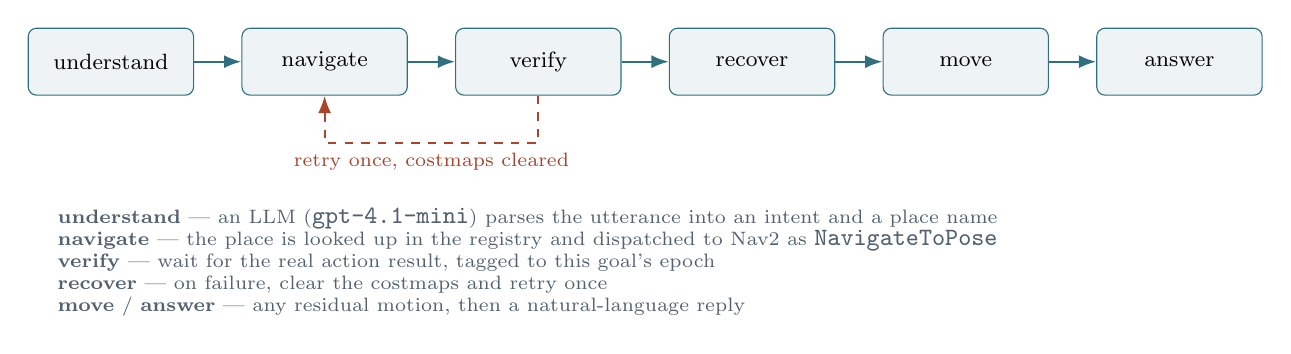
\begin{tikzpicture}[font=\small,node distance=6mm,
  nd/.style={draw=teal,fill=teal!8,rounded corners=3pt,minimum height=8.5mm,
             minimum width=21mm,align=center,font=\footnotesize},
  ar/.style={-{Latex[length=2.2mm]},teal,thick}]
\node[nd] (u) {understand};
\node[nd,right=of u] (n) {navigate};
\node[nd,right=of n] (v) {verify};
\node[nd,right=of v] (r) {recover};
\node[nd,right=of r] (m) {move};
\node[nd,right=of m] (a) {answer};
\draw[ar] (u)--(n); \draw[ar] (n)--(v); \draw[ar] (v)--(r);
\draw[ar] (r)--(m); \draw[ar] (m)--(a);
\draw[ar,rust,dashed] (v.south) -- ++(0,-6mm) -| (n.south)
  node[pos=0.25,below,font=\scriptsize,color=rust] {retry once, costmaps cleared};
\node[below=13mm of u,align=left,font=\scriptsize,color=slate,anchor=north west,xshift=-8mm]
  {\textbf{understand} --- an LLM (\file{gpt-4.1-mini}) parses the utterance into an
   intent and a place name\\
   \textbf{navigate} --- the place is looked up in the registry and dispatched to Nav2 as
   \file{NavigateToPose}\\
   \textbf{verify} --- wait for the real action result, tagged to this goal's epoch\\
   \textbf{recover} --- on failure, clear the costmaps and retry once\\
   \textbf{move} / \textbf{answer} --- any residual motion, then a natural-language reply};
\end{tikzpicture}
\caption[The command graph]{The LangGraph state machine that turns an
utterance into a Nav2 goal and back into an answer. Every transition is traced
to LangSmith, which is what makes the language layer auditable independently of
the navigation layer.}
\label{fig:langgraph}
\end{figure}

\begin{figure}[htbp]
\centering
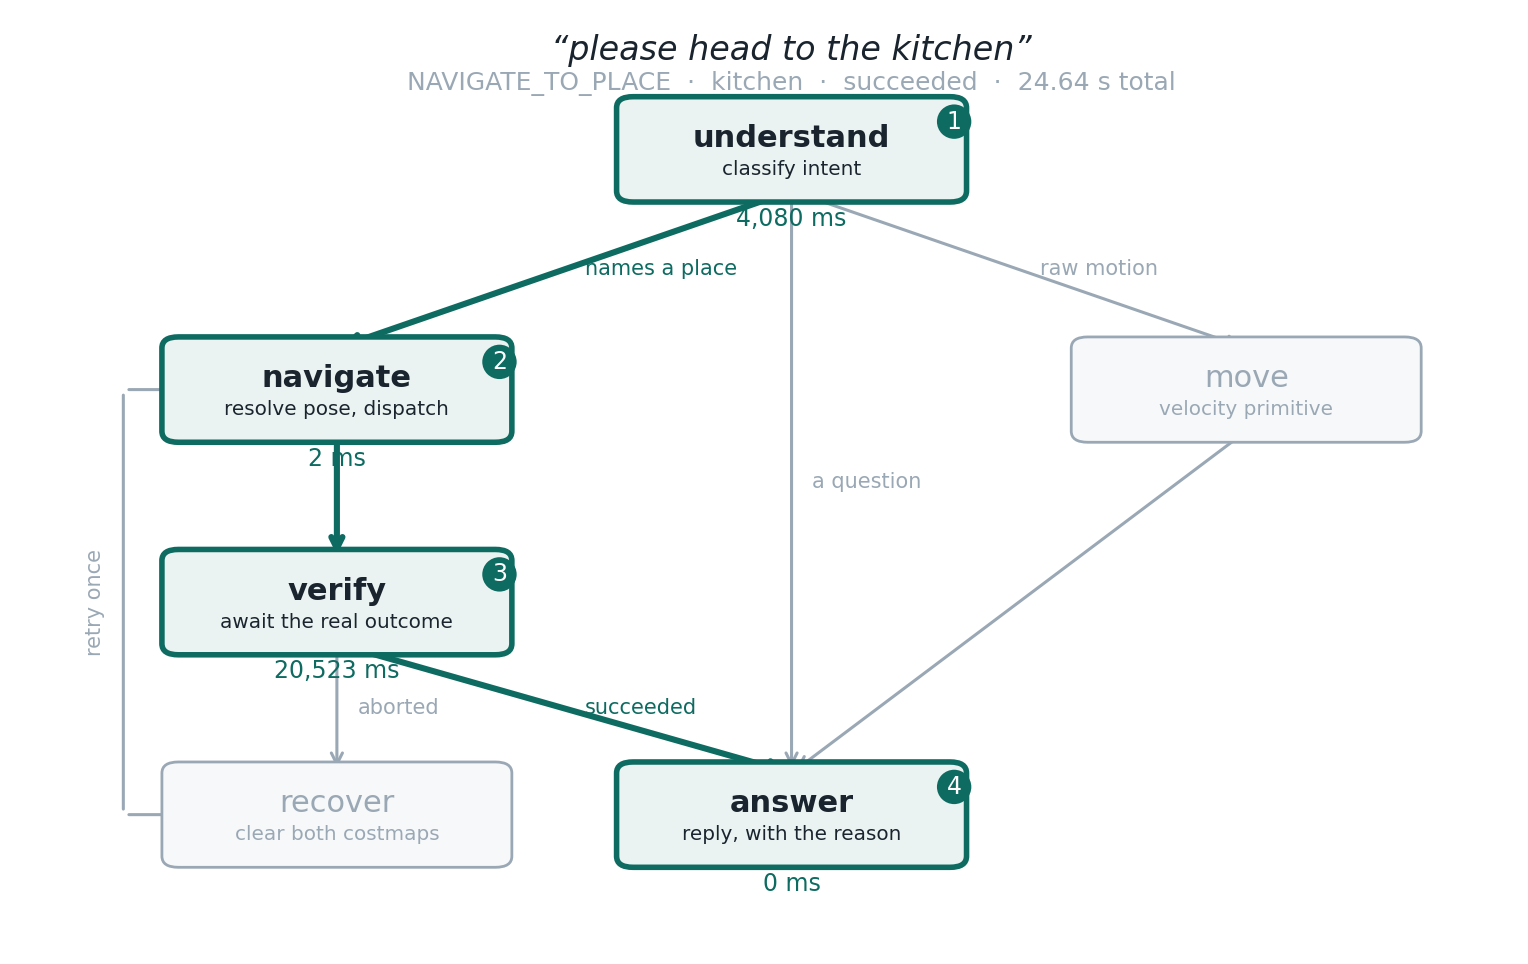
\includegraphics[width=0.86\textwidth]{fig/graph_trace.png}
\caption[A recorded trace]{One command executing through the graph, as
recorded. Regenerate with \file{scripts/plot\_trace.py} over
\file{backend/app/data/traces/graph\_runs.jsonl}.}
\label{fig:trace}
\end{figure}

\begin{plain}[The goal-epoch mechanism, and why it exists]
The \textbf{verify} node waits for the \file{NavigateToPose} result. Early in
the project it simply read the most recent outcome, and that is a bug: if a
goal is superseded, the old goal's result can still arrive and be attributed to
the new one. Each dispatch therefore now opens a numbered epoch, and a result
is only accepted if its epoch matches:

\begin{center}
\begin{minipage}{0.72\textwidth}
\ttfamily\footnotesize
def \_open\_goal(self) -> int:\\
\hspace*{1em}self.\_goal\_epoch += 1\\
\hspace*{1em}self.store.set(``nav\_outcome'', None)\\
\hspace*{1em}self.store.set(``is\_navigating'', True)\\
\hspace*{1em}return self.\_goal\_epoch
\end{minipage}
\end{center}
This is in \file{backend/app/services/ros2\_bridge.py} and it is one of the
four faults tabulated in Part~11.
\end{plain}

\begin{figure}[htbp]
\centering
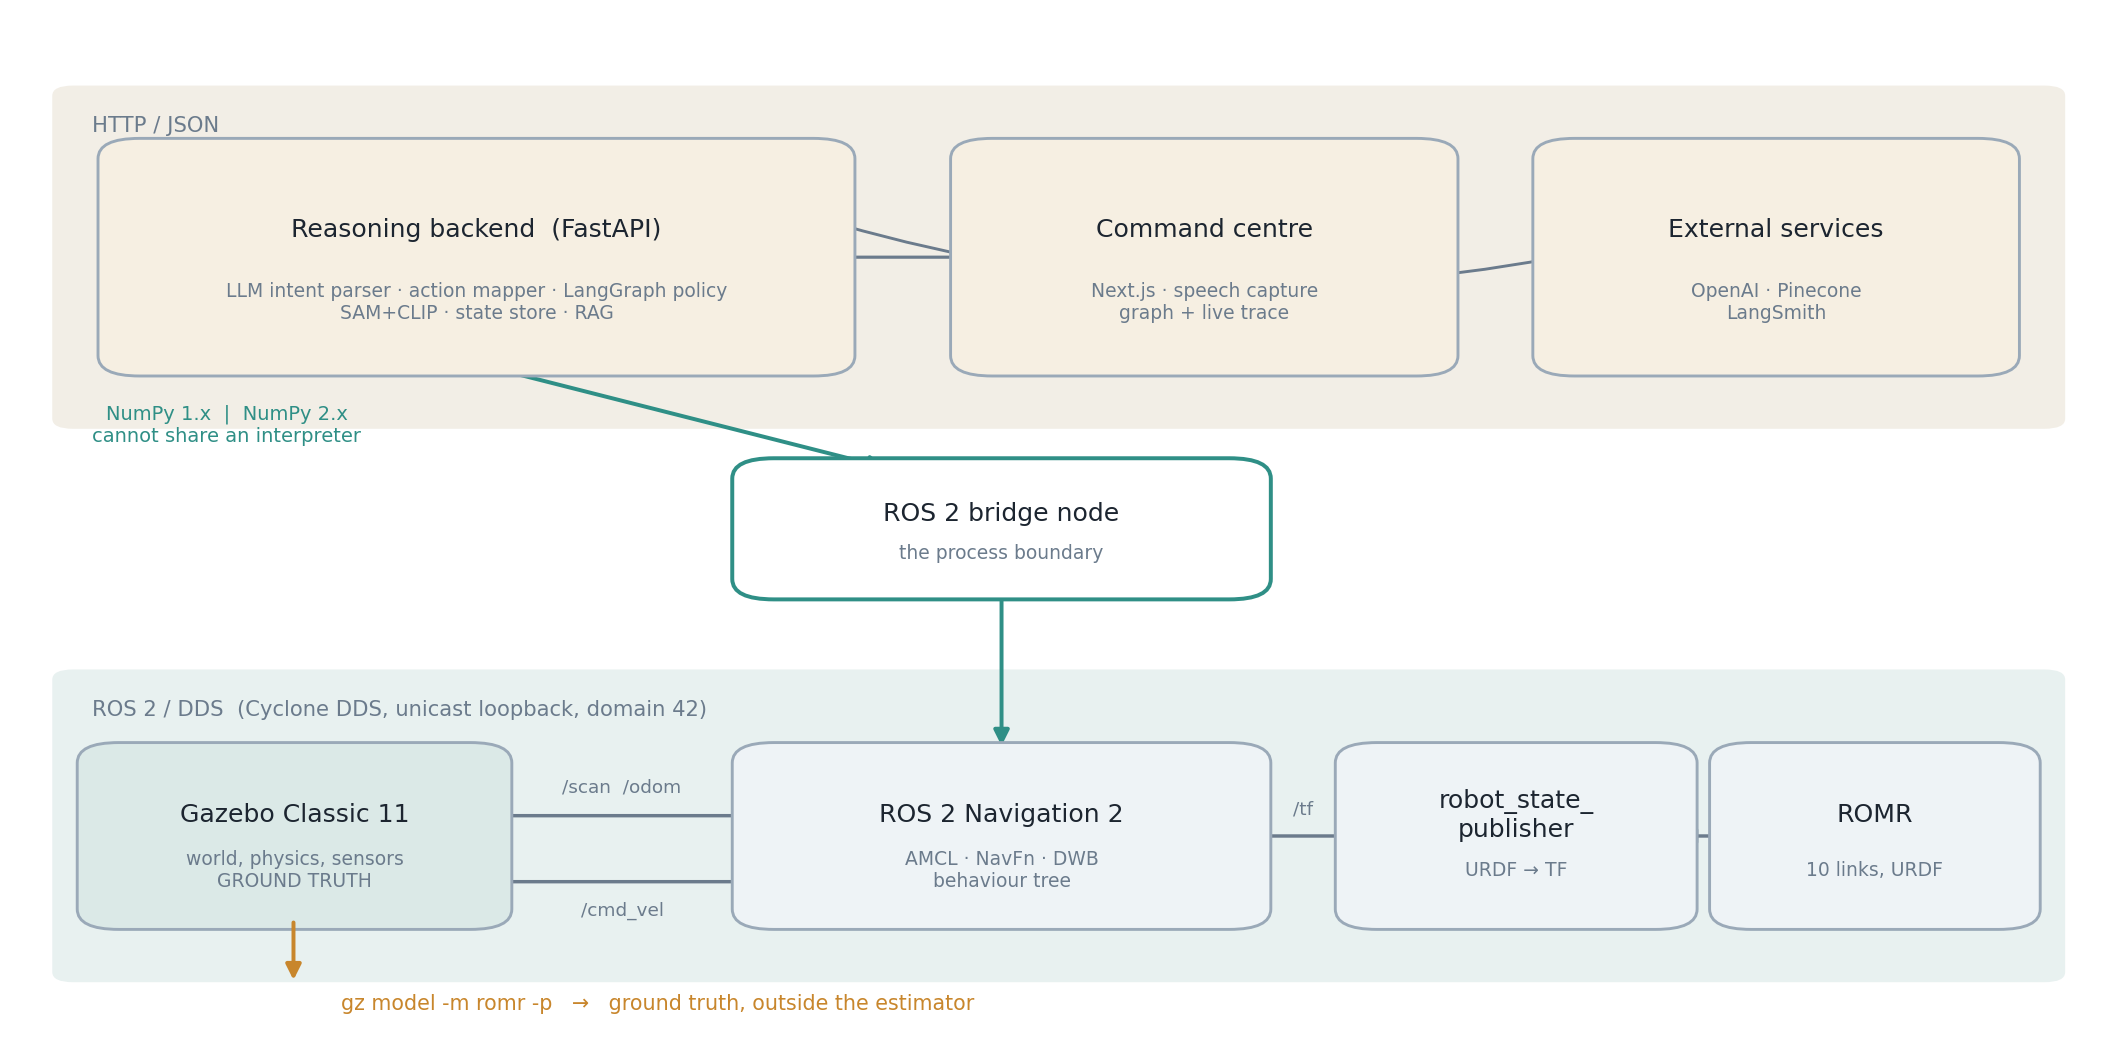
\includegraphics[width=\textwidth]{fig/system_arch.png}
\caption[The full system]{The complete system: language interface, reasoning
backend, perception, and the ROS~2 / Gazebo simulation. AMCL and Nav2 occupy
the right-hand portion; everything in this document concerns that portion and
the measurements taken across it.}
\label{fig:sysarch}
\end{figure}

% =========================================================================
\chapter{How the evaluation actually works}
\label{ch:eval}

Everything so far has been machinery. This part explains what was measured,
with what ruler, and why that ruler was chosen. It is written so that a
secondary-school student can follow it end to end.

\section{The one decision the whole evaluation rests on}

When you ask a robot to go to the kitchen and it says ``succeeded'', how do you
check?

The tempting answer is: look at where the robot says it is, and see if that is
near the kitchen. This is what almost every ROS tutorial does, and it is
worthless, because it asks the robot to mark its own homework. In the initial
run of this project it produced a $75\%$ success rate for a system that
actually arrived $19\%$ of the time.

The evaluation therefore uses an \term{external ruler}: the simulator's own
record of where the robot's body is. Gazebo knows this exactly, because Gazebo
is the thing computing it. It is read with a single command:
\begin{center}
\file{gz model -m romr -p}
\end{center}
which prints the model's true pose. The validation script parses $x$, $y$ and
yaw from it.

\begin{keyidea}[Ground truth]
\term{Ground truth} means: the real answer, obtained by a means independent of
the system under test. Here it is available only because this is a simulation.
On a physical robot it would require motion capture or a surveyed reference.
That the ground truth exists at all is the single biggest advantage of doing
this work in simulation, and it is why the false-positive rate could be
measured rather than guessed at.
\end{keyidea}

\section{Three distances, and the triangle between them}

For every trial the script records three numbers. Getting these three straight
is most of the work of understanding the results.

Let
\begin{itemize}[leftmargin=1.4em,itemsep=1pt]
\item $\mathbf{g} = (g_x, g_y)$ be the \textbf{goal} --- the registry
coordinates of the destination;
\item $\mathbf{t} = (t_x, t_y)$ be the \textbf{truth} --- where the robot's
body actually is, from Gazebo;
\item $\mathbf{b} = (b_x, b_y)$ be the \textbf{belief} --- where AMCL says the
robot is.
\end{itemize}

Then, using the ordinary distance formula from school geometry
$\;d = \sqrt{(\Delta x)^2 + (\Delta y)^2}\;$:

\begin{equation}
\begin{aligned}
e_{\text{true}} &= \lVert \mathbf{t} - \mathbf{g} \rVert
  = \sqrt{(t_x - g_x)^2 + (t_y - g_y)^2}
  && \text{\footnotesize how far the robot really is from the goal} \\[2pt]
e_{\text{AMCL}} &= \lVert \mathbf{b} - \mathbf{g} \rVert
  = \sqrt{(b_x - g_x)^2 + (b_y - g_y)^2}
  && \text{\footnotesize how far the robot \emph{thinks} it is from the goal} \\[2pt]
d_{\text{drift}} &= \lVert \mathbf{b} - \mathbf{t} \rVert
  = \sqrt{(b_x - t_x)^2 + (b_y - t_y)^2}
  && \text{\footnotesize how wrong the robot's self-knowledge is}
\end{aligned}
\label{eq:threedist}
\end{equation}

\begin{figure}[htbp]
\centering
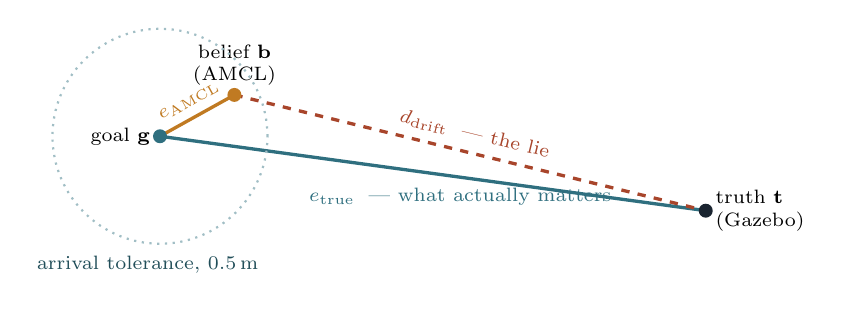
\begin{tikzpicture}[font=\small,scale=1.05]
\coordinate (G) at (0,0);
\coordinate (T) at (6.6,-0.9);
\coordinate (B) at (0.9,0.5);
\draw[teal,very thick] (G) -- node[below,font=\scriptsize,color=teal,pos=0.55]
  {$e_{\text{true}}$ \;--- what actually matters} (T);
\draw[amber,very thick] (G) -- node[above,font=\scriptsize,color=amber,pos=0.5,sloped]
  {$e_{\text{AMCL}}$} (B);
\draw[rust,very thick,dashed] (B) -- node[above,font=\scriptsize,color=rust,pos=0.5,sloped]
  {$d_{\text{drift}}$ \;--- the lie} (T);
\fill[teal] (G) circle (2.4pt); \node[left,font=\scriptsize] at (G) {goal $\mathbf{g}$};
\fill[ink]  (T) circle (2.4pt); \node[right,font=\scriptsize,align=left] at (T) {truth $\mathbf{t}$\\{\scriptsize(Gazebo)}};
\fill[amber](B) circle (2.4pt); \node[above,font=\scriptsize,align=center] at (B) {belief $\mathbf{b}$\\{\scriptsize(AMCL)}};
\draw[teal!45,dotted,thick] (G) circle (1.3);
\node[teal!70!black,font=\scriptsize] at (-0.15,-1.55) {arrival tolerance, \SI{0.5}{\metre}};
\end{tikzpicture}
\caption[The evaluation triangle]{The three distances of
equation~\eqref{eq:threedist}. In the initial run the belief sat inside the
tolerance circle while the truth sat metres outside it: Nav2 saw the amber
line, was satisfied, and reported success. The evaluation reports the teal
line.}
\label{fig:triangle}
\end{figure}

\begin{keyidea}[Why all three, and not just the first]
$e_{\text{true}}$ alone tells you the system failed. $e_{\text{true}}$
together with $e_{\text{AMCL}}$ tells you \emph{why}: if both are large, the
robot knew it had not arrived and navigation is at fault; if $e_{\text{true}}$
is large and $e_{\text{AMCL}}$ is small, navigation did its job faithfully and
\emph{localisation} is at fault. $d_{\text{drift}}$ measures that second case
directly. Recording all three is what allowed the failure to be attributed to
AMCL rather than to the planner, the language model or the map.
\end{keyidea}

\section{Arrival: what counts as having got there}

A trial counts as an \term{arrival} when
\[
e_{\text{true}} \le \SI{0.5}{\metre}.
\]

That threshold is not arbitrary. Nav2's own goal checker uses
\file{xy\_goal\_tolerance: 0.25}\,\si{\metre}; the evaluation deliberately uses
double that, so the scoring is \emph{more generous} than the stack's own test
and cannot be accused of manufacturing failures. Part~8 \S8.5 shows the result
is insensitive to the exact value.

\section{The command suite}

The suite lives in \file{scripts/validate\_commands.py}, in a dictionary named
\file{PHRASINGS}. Eight destinations, with multiple phrasings each --- $61$
commands in the corrected run.

\begin{center}
\small
\begin{tabular}{@{}lcp{8.4cm}@{}}
\toprule
\textbf{Destination} & \textbf{Goal $(x,y)$ in metres} & \textbf{Sample phrasings} \\
\midrule
\file{kitchen}        & $(-5.0793,\; 1.9436)$ & ``kitchen'', ``take yourself to the cooking area'' \\
\file{parlour}        & $(-4.5742,\; -1.0034)$& ``head to the lounge'', ``move to the living area'' \\
\file{waiting\_area}  & $(-0.0518,\; 0.4320)$ & ``head to reception'', ``please go to the lobby'' \\
\file{dining\_room}   & $(5.6325,\; 1.5407)$  & ``take me to the dinner table'' \\
\file{master\_bedroom}& $(5.1568,\; -2.1403)$ & ``navigate to the main bedroom'' \\
\file{garage}         & $(0.3124,\; -6.4615)$ & ``go park in the parking space'', ``car park'' \\
\file{store\_area}    & $(-3.9059,\; -6.2149)$& ``drive over to the storeroom'' \\
\file{home}           & $(-3.5378,\; -2.6976)$& ``take the robot to the docking station'' \\
\bottomrule
\end{tabular}
\end{center}

The phrasings are deliberately varied: bare nouns with no verb
(``\emph{kitchen}''), polite forms, registry aliases, indirect references
(``\emph{the docking station}''), and filler words that a brittle keyword
matcher would trip on. The purpose is to separate \emph{language
understanding} from \emph{navigation}: if the wrong place is resolved, that is
a language failure; if the right place is resolved and the robot does not
arrive, that is a navigation or localisation failure. The two are recorded in
separate columns (\file{resolved}, \file{correct}) and never conflated.

\section{Trial independence, and why re-seeding is itself a result}

Each trial begins correctly localised. Before dispatching a command the script
checks the gap between belief and truth, and if it exceeds \SI{1.0}{\metre} it
re-seeds AMCL from ground truth. If the robot has left the mapped region
entirely it is teleported back to the spawn pose. Both events are counted, and
the count is reported.

\begin{plain}[Why this is honest rather than convenient]
Without re-seeding, a single divergence poisons every subsequent trial. The
mechanism is a cascade: the robot follows a valid map-frame path into a wall;
its believed pose then lands inside an inflated costmap cell; and the planner
thereafter refuses \emph{every} goal, because it cannot plan from a start pose
it considers occupied. That is a real property of the system --- and it is
reported as such, in Part~8 \S8.3 --- but averaged into a per-command success
rate it would measure trial \emph{ordering} rather than language understanding.

Separating the two, and reporting the re-localisation count as its own number,
is the honest arrangement. In the corrected run the count is $0/61$: no trial
needed re-seeding, and the robot never left the map. That zero is itself one
of the strongest results in the study.
\end{plain}

\section{What the RViz window shows}

\begin{figure}[htbp]
\centering
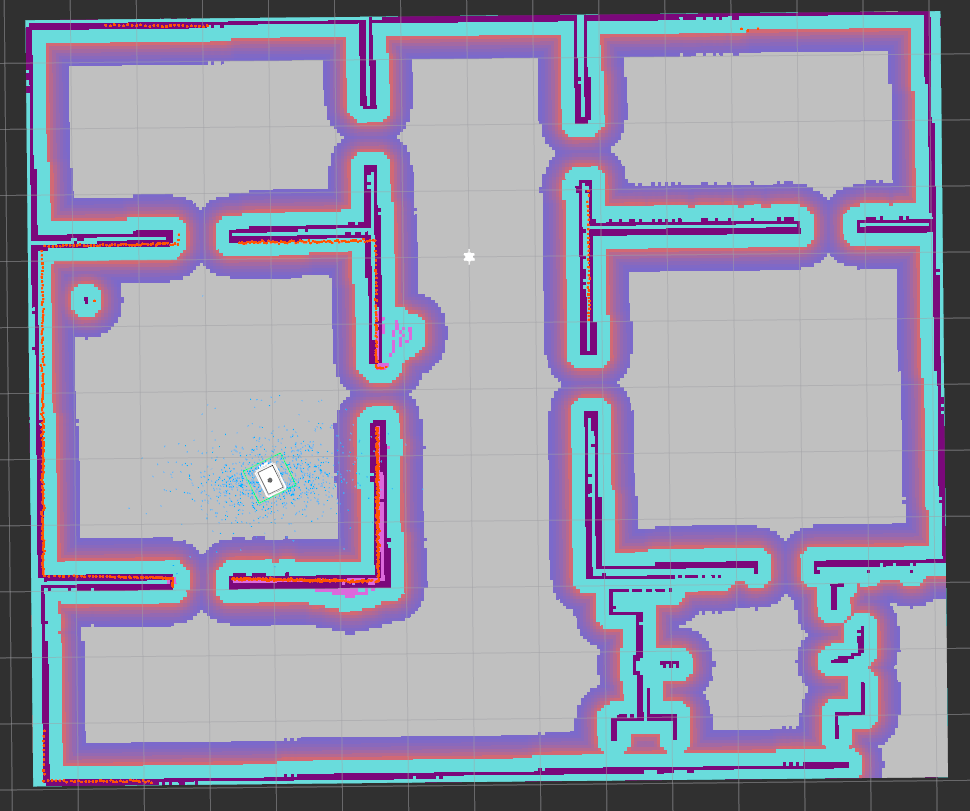
\includegraphics[width=0.78\textwidth]{fig/rviz.png}
\caption[RViz with AMCL running]{RViz during operation, viewed from directly
above. Everything discussed in Parts~3 to 6 is visible in this one window.
\textbf{Grey} is mapped free space and the dark outlines are walls, from the
static layer. The \textbf{cyan-to-purple-to-pink band} hugging every wall is
the inflation layer of equation~\eqref{eq:inflation} --- cyan is nearly lethal,
pink is the outer edge of the halo at \file{inflation\_radius} =
\SI{0.55}{\metre}; the planner will not route the robot through the cyan and
prefers to stay out of the purple. The \textbf{white rectangle} at mid-left is
the robot's published footprint, the \SI{0.521}{\metre} by \SI{0.608}{\metre}
polygon of \S6.3, drawn at the believed pose. The \textbf{blue speckle} spread
around it \emph{is} the particle set $\mathcal{X}_t$ of
equation~\eqref{eq:particleset} --- every dot is one complete hypothesis about
where the robot is. The \textbf{red and orange dots} along the walls are the
current laser scan, projected from the believed pose.}
\label{fig:rviz}
\end{figure}

\begin{center}
\small
\begin{tabular}{@{}lp{9.6cm}@{}}
\toprule
\textbf{What you see} & \textbf{What it is} \\
\midrule
Grey/black occupancy grid & the static map, \file{custom\_map\_v2} \\
Speckle of small dots     & the AMCL particle set; each dot is one
                            $(x,y,\theta)$ hypothesis. Its \emph{width} is
                            $\sigma$ made visible \\
White polygon             & the published footprint, at the believed pose \\
Red/orange dots on walls  & the current \file{/scan}, projected from the
                            believed pose \\
Cyan/purple/pink wash     & the inflation layer, equation~\eqref{eq:inflation};
                            cyan is nearest to lethal \\
Thin line to the goal     & the global plan from the Planner Server \\
\textbf{2D Pose Estimate} & publishes \file{/initialpose}; this is how you
                            re-seed AMCL by hand \\
\textbf{Nav2 Goal}        & publishes a \file{NavigateToPose} goal directly,
                            bypassing the language layer \\
\bottomrule
\end{tabular}
\end{center}

\begin{keyidea}[The single most useful thing to look at]
If the laser scan (the dots) lines up with the walls of the map, localisation
is working. If the scan is rotated or offset from the walls, it is not ---
\emph{regardless of what the pose estimate says}. The scan overlay is an
independent visual check of exactly the quantity equation~\eqref{eq:phit}
scores numerically.
\end{keyidea}

% =========================================================================
\chapter{Every number, worked by hand}
\label{ch:byhand}

This part reproduces the results tables from arithmetic you can do on paper.
For each table, at least two entries are computed in full. Where a number
cannot be obtained by hand --- because it requires processing hundreds of
laser beams, or running the filter --- the exact procedure is given instead,
with the command that produces it.

Two source files are used throughout:

\begin{center}
\small
\begin{tabular}{@{}lll@{}}
\toprule
\textbf{Run} & \textbf{File} & \textbf{Rows} \\
\midrule
Initial (before correction)   & \file{validation\_results\_groundtruth.csv} & 54 \\
Corrected (after correction)  & \file{results/validation\_2026-08-04\_fixed.csv} & 61 \\
\bottomrule
\end{tabular}
\end{center}

Both have the same eleven columns:
\begin{center}
\file{n}, \file{phrasing}, \file{expected}, \file{resolved}, \file{correct},
\file{outcome}, \file{error\_true\_m}, \file{error\_amcl\_m},
\file{amcl\_drift\_m}, \file{reseeded}, \file{seconds}.
\end{center}

\section{The distance formula, twice, on real coordinates}

Every $e$ and $d$ in the tables comes from one formula, the Pythagorean
distance:
\[
d = \sqrt{(x_2 - x_1)^2 + (y_2 - y_1)^2}.
\]

\begin{handbox}[Worked example 1: how far is the kitchen from home?]
From the place registry (\file{backend/app/data/places/new\_world\_places.yaml}):
\[
\text{home} = (-3.5378,\; -2.6976), \qquad
\text{kitchen} = (-5.0793,\; 1.9436).
\]
\textbf{Step 1 --- the differences.}
\[
\Delta x = -5.0793 - (-3.5378) = -1.5415,
\qquad
\Delta y = 1.9436 - (-2.6976) = 4.6412 .
\]
(Careful with the double negatives: subtracting a negative adds.)

\textbf{Step 2 --- square them.}
\[
(-1.5415)^2 = 2.376222, \qquad (4.6412)^2 = 21.540737 .
\]
\textbf{Step 3 --- add.}
\[
2.376222 + 21.540737 = 23.916960 .
\]
\textbf{Step 4 --- square root.}
\[
d = \sqrt{23.916960} = \SI{4.8905}{\metre}.
\]
\end{handbox}

\begin{handbox}[Worked example 2: parlour to garage]
\[
\text{parlour} = (-4.5742,\; -1.0034), \qquad
\text{garage} = (0.3124,\; -6.4615).
\]
\[
\Delta x = 0.3124 + 4.5742 = 4.8866, \qquad
\Delta y = -6.4615 + 1.0034 = -5.4581 .
\]
\[
4.8866^2 = 23.878860, \qquad (-5.4581)^2 = 29.790856 .
\]
\[
d = \sqrt{23.878860 + 29.790856} = \sqrt{53.669716} = \SI{7.3260}{\metre}.
\]
Note that squaring removes the sign: it does not matter which point you call
first.
\end{handbox}

These are distances between two \emph{known} points. In the results,
$e_{\text{true}}$ is the same formula applied between the goal and the robot's
Gazebo pose, and $e_{\text{AMCL}}$ between the goal and AMCL's pose. The CSV
stores the resulting distances rather than the raw poses, so the individual
$(x,y)$ values are not recoverable from it --- which is why the next section
uses a different, and arguably stronger, check.

\section{Checking the recorded data against itself}

Even without the raw poses, the three recorded distances must obey the
\term{triangle inequality}: for any three points, no side of the triangle they
form can be longer than the other two added together, nor shorter than their
difference.
\begin{equation}
\bigl| e_{\text{true}} - e_{\text{AMCL}} \bigr|
\;\;\le\;\; d_{\text{drift}} \;\;\le\;\;
e_{\text{true}} + e_{\text{AMCL}} .
\label{eq:triangle}
\end{equation}

This is a real audit: if the columns had been recorded at inconsistent moments
--- if the robot had moved between reading its belief and reading its truth ---
equation~\eqref{eq:triangle} would fail.

\begin{handbox}[Two trials checked]
\textbf{Trial 18, initial run, ``take me to the dining room''.}
Recorded: $e_{\text{true}} = 15.631$, $e_{\text{AMCL}} = 0.241$,
$d_{\text{drift}} = 15.432$.
\[
\bigl|15.631 - 0.241\bigr| = 15.390,
\qquad 15.631 + 0.241 = 15.872 .
\]
Is $15.390 \le 15.432 \le 15.872$? Yes. \checkmark

\smallskip
\textbf{Trial 43, initial run, ``head to the dining area''.}
Recorded: $15.664$, $0.208$, $15.465$.
\[
\bigl|15.664 - 0.208\bigr| = 15.456,
\qquad 15.664 + 0.208 = 15.872 .
\]
Is $15.456 \le 15.465 \le 15.872$? Yes. \checkmark

\smallskip
\textbf{What the near-equality tells you.} In both cases $d_{\text{drift}}$ is
only just above the lower bound. A triangle whose third side almost equals the
difference of the other two is almost \emph{flat}: the three points are nearly
in a straight line, with the belief sitting between the goal and the truth,
right next to the goal.

Quantify it with the law of cosines. The angle at the belief vertex is
\[
\cos\phi = \frac{e_{\text{AMCL}}^2 + d_{\text{drift}}^2 - e_{\text{true}}^2}
                {2\, e_{\text{AMCL}}\, d_{\text{drift}}} .
\]
For trial 43:
\[
\cos\phi = \frac{0.208^2 + 15.465^2 - 15.664^2}{2 \times 0.208 \times 15.465}
= \frac{0.043 + 239.167 - 245.361}{6.433}
= \frac{-6.151}{6.433} = -0.9562,
\]
so $\phi = \ang{163.0}$ --- nearly a straight line.

\textbf{The physical meaning}: AMCL had planted its belief essentially
\emph{on the goal}, and the robot was fifteen and a half metres away along
almost exactly the line from the goal through the belief. This is not a filter
that is unsure. It is a filter that has confidently converged on the wrong
place. Compare Part~3 \S3.2.3 on the support condition.
\end{handbox}

\section{Table --- validity audit: 16 trials, not 54}
\label{sec:hand-audit}

The initial run has $54$ rows, but only some of them represent a navigation
that actually ran. The audit splits them by duration.

\begin{center}
\begin{tabular}{@{}lcc@{}}
\toprule
 & $\ge \SI{10}{\second}$ & $< \SI{10}{\second}$ \\
\midrule
Trials & \textbf{16} & \textbf{38} \\
Reported success & \textbf{12} & \textbf{0} \\
Arrived ($e_{\text{true}} \le \SI{0.5}{\metre}$) & \textbf{3} & \textbf{0} \\
Median $e_{\text{true}}$ (\si{\metre}) & \textbf{6.35} & \textbf{5.98} \\
Median $d_{\text{drift}}$ (\si{\metre}) & \textbf{6.25} & \textbf{0.54} \\
\bottomrule
\end{tabular}
\end{center}

\begin{handbox}[Entry 1: the split, 16 and 38]
Read the \file{seconds} column of \file{validation\_results\_groundtruth.csv}
and sort it. The values fall into two clearly separated groups:

\emph{Short group} --- $4.4, 4.4, 4.8, 4.9, \ldots, 5.8, 9.9$ seconds. These
are trials where the planner refused the goal immediately: the command was
parsed, dispatched, and rejected in about five seconds. Counting them:
\textbf{38}.

\emph{Long group} --- these sixteen, in seconds:
\[
\begin{aligned}
&25.2,\ 26.0,\ 27.8,\ 63.7,\ 64.3,\ 67.6,\ 74.2,\ 76.1,\\
&83.2,\ 86.8,\ 88.8,\ 94.7,\ 94.9,\ 95.4,\ 131.9,\ 143.4 .
\end{aligned}
\]
Counting them: \textbf{16}.

$38 + 16 = 54$. \checkmark\; There is no trial between \SI{9.9}{\second} and
\SI{25.2}{\second}, so the \SI{10}{\second} cut is unambiguous.
\end{handbox}

\begin{handbox}[Entry 2: median $e_{\text{true}}$ for the 16-trial group]
The sixteen true errors, sorted (metres):
\[
\begin{aligned}
&0.330,\ 0.426,\ 0.467,\ 1.693,\ 2.071,\ 5.127,\ 5.182,\ \mathbf{5.202},\\
&\mathbf{7.491},\ 7.524,\ 8.733,\ 8.793,\ 11.264,\ 15.612,\ 15.631,\ 15.664 .
\end{aligned}
\]
$16$ is even, so the median is the mean of the $8$th and $9$th:
\[
\frac{5.202 + 7.491}{2} = \frac{12.693}{2} = 6.3465 \;\rightarrow\; \SI{6.35}{\metre}. \;\checkmark
\]
\end{handbox}

\begin{handbox}[Entry 3: median $d_{\text{drift}}$ for the same group]
The sixteen drifts, sorted (metres):
\[
\begin{aligned}
&0.394,\ 0.531,\ 0.576,\ 2.524,\ 2.677,\ 4.982,\ 5.035,\ \mathbf{5.295},\\
&\mathbf{7.204},\ 7.221,\ 8.668,\ 8.702,\ 11.132,\ 15.204,\ 15.432,\ 15.465 .
\end{aligned}
\]
\[
\frac{5.295 + 7.204}{2} = \frac{12.499}{2} = 6.2495 \;\rightarrow\; \SI{6.25}{\metre}. \;\checkmark
\]
\end{handbox}

\begin{keyidea}[Why the audit matters]
All $12$ reported successes are in the $16$-trial group; the $38$ short trials
reported nothing. So the false-positive rate is a statement about the $16$, and
reporting it over all $54$ would dilute it with trials that never navigated.
This is a deliberate narrowing that makes the headline number \emph{worse}, not
better, and it is the right thing to do.
\end{keyidea}

\section{Table --- reported versus actual arrival, initial run}

\begin{center}
\begin{tabular}{@{}lcc@{}}
\toprule
\textbf{Quantity} & \textbf{Count} & \textbf{Rate} \\
\midrule
Trials & 16 & --- \\
Reported success by the stack & 12 & $75\%$ \\
Arrived within \SI{0.5}{\metre} & 2 of those 12 & $17\%$ \\
Reported success that was false & 10 of 12 & $\mathbf{83\%}$ \\
\bottomrule
\end{tabular}
\end{center}

\begin{handbox}[Entry 1: the $75\%$]
Count rows in the $16$-trial group whose \file{outcome} column reads
\file{succeeded}. They are trials
$18, 19, 20, 21, 22, 38, 39, 40, 41, 42, 43, 44$ --- twelve of them.
\[
\frac{12}{16} = 0.75 = 75\% . \;\checkmark
\]
\end{handbox}

\begin{handbox}[Entry 2: the $17\%$ and the $83\%$]
Take those same twelve rows and read their $e_{\text{true}}$:
\begin{center}
\small
\begin{tabular}{@{}rlrl@{}}
\toprule
$n$ & phrasing & $e_{\text{true}}$ & $\le \SI{0.5}{\metre}$? \\
\midrule
18 & take me to the dining room & 15.631 & no \\
19 & please move to the garage  &  8.793 & no \\
20 & go park in the garage      &  8.733 & no \\
21 & go to the storage area     &  5.127 & no \\
22 & navigate home              &  \textbf{0.467} & \textbf{yes} \\
38 & please go to the store area&  5.202 & no \\
39 & move to storage            &  5.182 & no \\
40 & I need you in the kitchen  &  7.491 & no \\
41 & please head to the kitchen &  7.524 & no \\
42 & move to the living room    & 11.264 & no \\
43 & head to the dining area    & 15.664 & no \\
44 & head back home             &  \textbf{0.426} & \textbf{yes} \\
\bottomrule
\end{tabular}
\end{center}
Two ``yes'' out of twelve:
\[
\frac{2}{12} = 0.1667 = 16.7\% \approx 17\% \;\checkmark
\]
and therefore
\[
\frac{10}{12} = 0.8333 = 83.3\% \approx 83\% \text{ false.} \;\checkmark
\]

\textbf{Read the table above once more.} Both of the genuine arrivals are
\emph{home}, which is only \SI{0.96}{\metre} from the spawn pose --- the robot
barely had to move, so odometry barely had a chance to drift. Every trial that
required a real journey failed. That single observation is the diagnosis, and
it is visible from arithmetic alone.
\end{handbox}

\section{Table --- arrivals as a function of the threshold}

\begin{center}
\begin{tabular}{@{}lcccc@{}}
\toprule
Threshold (\si{\metre}) & 0.3 & 0.5 & 0.6 & 1.0 \\
\midrule
Arrivals & 0 & 3 & 3 & 4 \\
\bottomrule
\end{tabular}
\end{center}

The point of this table is to show the headline result does not depend on
where the arrival line is drawn.

\begin{handbox}[All four entries, by hand]
Sort every $e_{\text{true}}$ in the initial run and look at the small end:
\[
0.330,\quad 0.426,\quad 0.467,\quad 0.681,\quad 1.693,\quad 1.782,\ \ldots
\]
Now count how many are $\le$ each threshold:
\begin{itemize}[leftmargin=1.4em,itemsep=1pt]
\item $\le 0.3$: none. The smallest is $0.330$. \textbf{0} \checkmark
\item $\le 0.5$: $0.330,\; 0.426,\; 0.467$. \textbf{3} \checkmark
\item $\le 0.6$: the same three; $0.681$ is above. \textbf{3} \checkmark
\item $\le 1.0$: those three, plus $0.681$. \textbf{4} \checkmark
\end{itemize}
Even at double the chosen tolerance, four arrivals out of fifty-four.
\end{handbox}

\begin{warnbox}[A discrepancy worth fixing before publication]
This particular table is computed over \emph{all 54} rows, whereas the
surrounding text works over the \emph{16}-trial group. The two agree at
$0.3$, $0.5$ and $0.6$, but differ at $1.0$: over the 16-trial group the count
is $3$, not $4$, because the fourth arrival ($e_{\text{true}} = 0.681$,
trial~17, ``take the robot home'') is a $\SI{5.0}{\second}$ trial that never
navigated. Either denominator is defensible; \emph{stating which one is used}
is not optional. The caption should read ``over all 54 trials'' or the $1.0$
column should read $3$.
\end{warnbox}

\section{Table --- before and after correction}

\begin{center}
\small
\begin{tabular}{@{}lcc@{}}
\toprule
\textbf{Measure} & \textbf{Initial} & \textbf{Corrected} \\
\midrule
Trials analysed & 16 & 61 \\
Intent resolved correctly & $100\%$ & $60/61$ ($98\%$) \\
Reported success & 12 ($75\%$) & 50 ($82\%$) \\
Arrived within \SI{0.5}{\metre} & 3 & \textbf{60 ($98\%$)} \\
False positives among reported & $10/12$ ($83\%$) & $\mathbf{0/50}$ \\
Median $e_{\text{true}}$ (\si{\metre}) & 6.35 & \textbf{0.231} \\
Mean $e_{\text{true}}$ (\si{\metre}) & --- & 0.259 \\
Maximum $e_{\text{true}}$ (\si{\metre}) & 15.66 & 0.483 \\
Median $d_{\text{drift}}$ (\si{\metre}) & 6.25 & 0.108 \\
Mean $d_{\text{drift}}$ (\si{\metre}) & 6.94 & 0.189 \\
Median trial duration (\si{\second}) & 5.1 & 57.2 \\
Re-localisations required & --- & $0/61$ \\
\bottomrule
\end{tabular}
\end{center}

\begin{handbox}[Entry 1: median $e_{\text{true}}$ of the corrected run $= 0.231$]
Sixty of the $61$ rows have an $e_{\text{true}}$ (trial~49 resolved no place,
so no error could be computed --- see the next box). Sorted, the middle of the
list reads:
\[
\ldots,\ 0.222,\ 0.224,\ 0.228,\ \mathbf{0.230},\ \mathbf{0.232},\ 0.238,\ 0.244,\ 0.249,\ \ldots
\]
With $60$ values the median is the mean of the $30$th and $31$st:
\[
\frac{0.230 + 0.232}{2} = \frac{0.462}{2} = \SI{0.231}{\metre}. \;\checkmark
\]
\end{handbox}

\begin{handbox}[Entry 2: mean $e_{\text{true}}$ of the corrected run $= 0.259$]
Sum all $60$ values and divide by $60$. The total is $\SI{15.551}{\metre}$:
\[
\bar{e} = \frac{15.551}{60} = 0.25918 \;\rightarrow\; \SI{0.259}{\metre}. \;\checkmark
\]
Note $\text{mean} > \text{median}$ ($0.259$ against $0.231$), as always when a
distribution has a longer tail on the high side. The gap is small here ---
$\SI{0.028}{\metre}$ --- because the corrected run has no outliers. In the
initial run the same gap was $\SI{0.60}{\metre}$ on a median of $\SI{6.35}{}$.
\end{handbox}

\begin{handbox}[Entry 3: the $98\%$ arrival rate]
Count rows in the corrected run with $e_{\text{true}} \le 0.5$. The maximum
recorded value is $0.483$ (trial~45), so \emph{every} row that has a value at
all passes. That is $60$.
\[
\frac{60}{61} = 0.98360 \approx 98\% . \;\checkmark
\]
The one that does not is trial~49, ``drive to the store'', where
\file{resolved} is empty and \file{outcome} is \file{dispatched}. That is a
\emph{language} failure: the phrase ``the store'' did not resolve to
\file{store\_area}, so no goal was ever sent and no distance exists to measure.
It is counted against the system --- $60/61$, not $60/60$ --- which is the
conservative choice.
\end{handbox}

\begin{handbox}[Entry 4: median $d_{\text{drift}} = 0.108$]
Here all $61$ rows have a value, including trial~49 (drift does not need a
goal --- it is belief against truth). $61$ is odd, so the median is simply the
$31$st value of the sorted list, which is $\SI{0.108}{\metre}$. \checkmark

Compare with the initial run's $\SI{6.25}{\metre}$: a factor of
$6.25 / 0.108 = \mathbf{58}$ reduction in how badly the robot misunderstood
its own position.
\end{handbox}

\begin{handbox}[Entry 5: median duration $5.1 \rightarrow \SI{57.2}{\second}$]
Initial run, all $54$ durations sorted: the $27$th and $28$th are both
$\SI{5.1}{\second}$, so the median is $\SI{5.1}{\second}$. \checkmark

Corrected run, $61$ durations sorted: the $31$st is $\SI{57.2}{\second}$. \checkmark

\textbf{This row is not padding.} A median of five seconds means the typical
initial trial \emph{never navigated at all} --- it was refused by the planner.
A median of fifty-seven seconds means the typical corrected trial drove across
the building. The two runs are not comparing good navigation with bad
navigation; they are comparing navigation with its absence.
\end{handbox}

\section{The pattern nobody had looked for: error against distance}
\label{sec:hand-distance}

Every table so far reports a single number for the whole run. That hides
something, and what it hides turns out to be the clearest signal in the entire
dataset.

Take the 16 valid trials of the initial run, group them by which room was
asked for, and sort the groups by how far that room is from where the robot
starts, at $(-2.92,\, -3.43)$.

\begin{handbox}[The two distances, by hand]
\textbf{Furthest --- the dining room}, at $(5.6325,\, 1.5407)$:
\begin{align*}
\Delta x &= 5.6325 - (-2.92) = 8.5525, &
\Delta y &= 1.5407 - (-3.43) = 4.9707 \\
\Delta x^2 &= 73.1453, &
\Delta y^2 &= 24.7079
\end{align*}
\[
d = \sqrt{73.1453 + 24.7079} = \sqrt{97.8532} = \SI{9.89}{\metre}.
\]

\textbf{Nearest --- home}, at $(-3.5378,\, -2.6976)$:
\begin{align*}
\Delta x &= -3.5378 - (-2.92) = -0.6178, &
\Delta y &= -2.6976 - (-3.43) = 0.7324 \\
\Delta x^2 &= 0.3817, &
\Delta y^2 &= 0.5364
\end{align*}
\[
d = \sqrt{0.3817 + 0.5364} = \sqrt{0.9181} = \SI{0.96}{\metre}.
\]
\end{handbox}

\begin{center}
\small
\begin{tabular}{@{}lccccc@{}}
\toprule
\textbf{Destination} & \textbf{Distance} & \textbf{Trials} &
\textbf{Median error} & \textbf{Range} & \textbf{Ranks} \\
 & (\si{\metre}) & & (\si{\metre}) & (\si{\metre}) & $d$ / $e$ \\
\midrule
\file{home}         & 0.96 & 3 & 0.43  & 0.33--0.47  & 1 / 1 \\
\file{parlour}      & 2.94 & 2 & 6.67  & 2.07--11.26 & 2 / 3 \\
\file{store\_area}  & 2.95 & 4 & 5.15  & 1.69--5.20  & 3 / 2 \\
\file{garage}       & 4.43 & 2 & 8.76  & 8.73--8.79  & 4 / 5 \\
\file{kitchen}      & 5.79 & 2 & 7.51  & 7.49--7.52  & 5 / 4 \\
\file{dining\_room} & 9.89 & 3 & 15.63 & 15.61--15.66 & 6 / 6 \\
\bottomrule
\end{tabular}
\end{center}

Read the last column downwards. The order of the rooms by distance and the
order of the rooms by error are \emph{almost the same list}. Only two adjacent
pairs are swapped.

\subsection{Putting a number on ``almost the same list''}

A \term{correlation coefficient} is one number saying how closely two
quantities move together. It runs from $-1$ (perfect opposition) through $0$
(no relationship) to $+1$ (perfect agreement).

The easiest one to compute by hand is \term{Spearman's rank correlation}
$\rho$, which ignores the actual values and looks only at the \emph{ordering}.
That is exactly what we want here. Its formula, when no two ranks tie, is
\begin{equation}
\rho = 1 - \frac{6 \sum_{i} d_i^{\,2}}{n\,(n^2 - 1)},
\label{eq:spearman}
\end{equation}
where $d_i$ is the difference between the two ranks of item $i$, and $n$ is
how many items there are.

\begin{handbox}[Spearman's $\rho$ over the six destinations]
Take the rank differences straight from the table's last column:
\begin{center}\small
\begin{tabular}{@{}lccc@{}}
\toprule
Destination & rank by $d$ & rank by $e$ & $d_i$ \quad $d_i^{\,2}$ \\
\midrule
\file{home}         & 1 & 1 & $0$ \quad 0 \\
\file{parlour}      & 2 & 3 & $-1$ \quad 1 \\
\file{store\_area}  & 3 & 2 & $+1$ \quad 1 \\
\file{garage}       & 4 & 5 & $-1$ \quad 1 \\
\file{kitchen}      & 5 & 4 & $+1$ \quad 1 \\
\file{dining\_room} & 6 & 6 & $0$ \quad 0 \\
\midrule
 & & $\sum d_i^{\,2}$ & $\mathbf{4}$ \\
\bottomrule
\end{tabular}
\end{center}
With $n = 6$:
\[
\rho = 1 - \frac{6 \times 4}{6 \times (36 - 1)}
     = 1 - \frac{24}{210}
     = 1 - 0.1143
     = \mathbf{0.886}. \;\checkmark
\]
Scored over the 16 individual trials rather than the six room averages, the
same coefficient is $0.821$ and the ordinary linear correlation is $0.911$.
Those are the two figures quoted in the thesis.
\end{handbox}

\begin{warnbox}[What a correlation does \emph{not} tell you]
A high $\rho$ says two orderings agree. It does not say one causes the other,
and it does not license a significance test here --- there are six rooms, they
were not randomly chosen, and the trials within a room are not independent of
one another. The coefficient is quoted as a compact description of the table
above it, nothing more. The table is the evidence; the number is shorthand.
\end{warnbox}

\subsection{Why this matters more than the coefficient does}

Forget the statistics for a moment and look at the raw trials.

\begin{itemize}[leftmargin=1.4em,itemsep=3pt]
\item All three \file{dining\_room} trials --- the furthest room, at
\SI{9.89}{\metre} --- finished \SI{15.61}{}, \SI{15.63}{} and
\SI{15.66}{\metre} from the goal. That is a spread of \SI{0.05}{\metre}
across three independent runs.
\item All three \file{home} trials --- the nearest room, at \SI{0.96}{\metre}
--- finished \SI{0.33}{}, \SI{0.43}{} and \SI{0.47}{\metre} from the goal.
\end{itemize}

Same map. Same parameter file. Same afternoon. The only thing that differed
was how far the robot had to travel.

\begin{keyidea}[This distinguishes two kinds of fault]
A fault \emph{in the map} belongs to a place. A wall drawn in the wrong spot
ruins one room and leaves the others alone --- and it does not care how far
away that room is.

A fault \emph{in the model} --- in the odometry noise settings, or in the
laser range assumption --- belongs to the \emph{path}. Its effect accumulates
with every metre driven. Twice the distance, roughly twice the error.

The table shows error tracking distance almost perfectly. That is the
signature of the second kind, and it is why \S8.10 goes on to measure the
sensor and motion models rather than re-examining the map. The stability of
the dining-room trials points the same way, for the reason given in
\S\ref{sec:slam-vs-amcl}: a filter that has settled on a wrong answer returns
to that same wrong answer every time.
\end{keyidea}

\subsection{And after the corrections}

Run the same analysis on the corrected data and the pattern is gone. The
linear correlation falls from $0.911$ to $0.147$; the rank correlation from
$0.821$ to $0.121$. The eight \file{dining\_room} trials --- still the
furthest room --- finish between \SI{0.16}{} and \SI{0.42}{\metre} from the
goal, which is the same band as every other room in the house.

\begin{warnbox}[Be honest about why that number is small]
The correlation collapsed partly because there is nothing left for distance to
explain: \emph{no} trial in the corrected run missed by more than
\SI{0.483}{\metre}, at any range. When every value is squeezed into a band a
few centimetres wide, a correlation coefficient has almost nothing to bite on.

So the defensible claim is \textbf{``large errors at long range have
disappeared''}, not ``distance and error are now proven independent''. The
first is what the data shows. The second would need failures deliberately
induced across a range of distances, which is a study that has not been run.
\end{warnbox}

\section{Table --- the confusion matrix, precision and recall}
\label{sec:hand-confusion}

This is the table that carries the argument, so it is worked in full.

Treat the stack's ``succeeded'' report as a \emph{decision} about whether the
robot arrived, and score that decision against ground truth. Four outcomes are
possible.

\begin{figure}[htbp]
\centering
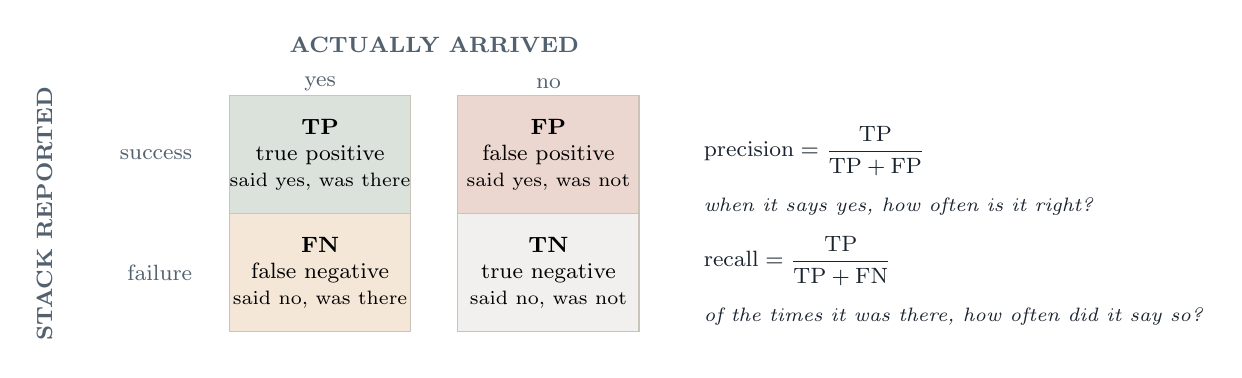
\begin{tikzpicture}[font=\small]
\node[font=\footnotesize\bfseries,color=slate] at (2.6,2.15) {ACTUALLY ARRIVED};
\node[font=\footnotesize\bfseries,color=slate,rotate=90] at (-2.35,0) {STACK REPORTED};
\node[font=\footnotesize,color=slate] at (1.15,1.65) {yes};
\node[font=\footnotesize,color=slate] at (4.05,1.65) {no};
\node[font=\footnotesize,color=slate,anchor=east] at (-0.35,0.75) {success};
\node[font=\footnotesize,color=slate,anchor=east] at (-0.35,-0.75) {failure};
\draw[fill=sage!22,draw=rule] (0,0) rectangle (2.3,1.5);
\node[align=center,font=\footnotesize] at (1.15,0.75) {\textbf{TP}\\true positive\\{\scriptsize said yes, was there}};
\draw[fill=rust!22,draw=rule] (2.9,0) rectangle (5.2,1.5);
\node[align=center,font=\footnotesize] at (4.05,0.75) {\textbf{FP}\\false positive\\{\scriptsize said yes, was not}};
\draw[fill=amber!18,draw=rule] (0,-1.5) rectangle (2.3,0);
\node[align=center,font=\footnotesize] at (1.15,-0.75) {\textbf{FN}\\false negative\\{\scriptsize said no, was there}};
\draw[fill=rule!25,draw=rule] (2.9,-1.5) rectangle (5.2,0);
\node[align=center,font=\footnotesize] at (4.05,-0.75) {\textbf{TN}\\true negative\\{\scriptsize said no, was not}};
\node[align=left,font=\footnotesize,anchor=west,color=ink] at (5.9,0.55)
 {$\text{precision} = \dfrac{\mathrm{TP}}{\mathrm{TP}+\mathrm{FP}}$\\[7pt]
  {\scriptsize \emph{when it says yes, how often is it right?}}};
\node[align=left,font=\footnotesize,anchor=west,color=ink] at (5.9,-0.85)
 {$\text{recall} = \dfrac{\mathrm{TP}}{\mathrm{TP}+\mathrm{FN}}$\\[7pt]
  {\scriptsize \emph{of the times it was there, how often did it say so?}}};
\end{tikzpicture}
\caption[The confusion matrix]{The four possible outcomes of treating a
success report as a decision, and the two rates computed from them. Precision
is a property of the \emph{claims}; recall is a property of the
\emph{opportunities}.}
\label{fig:confusion}
\end{figure}

\begin{center}
\begin{tabular}{@{}lcc@{}}
\toprule
 & \textbf{Initial} ($n=16$) & \textbf{Corrected} ($n=61$) \\
\midrule
True positives  & 2  & 50 \\
False positives & 10 & \textbf{0} \\
False negatives & 1  & \textbf{10} \\
True negatives  & 3  & 1 \\
\midrule
Precision & 0.167 & \textbf{1.000} \\
Recall    & 0.667 & 0.833 \\
\bottomrule
\end{tabular}
\end{center}

\begin{handbox}[The initial run, all six numbers]
\textbf{Step 1 --- classify each of the 16 trials.} Reported success:
$12$ trials. Arrived ($e_{\text{true}} \le 0.5$): $3$ trials, namely
$n = 1$ ($0.330$), $n = 22$ ($0.467$), $n = 44$ ($0.426$).

\smallskip
\textbf{Step 2 --- cross-tabulate.}
\begin{itemize}[leftmargin=1.4em,itemsep=1pt]
\item TP = reported \emph{and} arrived. Of the three arrivals, $22$ and $44$
were reported; $n = 1$ was \file{aborted}. So \textbf{TP} $= 2$.
\item FP = reported \emph{but did not} arrive. $12 - 2 = \mathbf{10}$.
\item FN = arrived \emph{but not} reported. $3 - 2 = \mathbf{1}$ (that is
$n = 1$, ``go home'').
\item TN = neither. $16 - 2 - 10 - 1 = \mathbf{3}$.
\end{itemize}
Check: $2 + 10 + 1 + 3 = 16$. \checkmark

\smallskip
\textbf{Step 3 --- precision.}
\[
\text{precision} = \frac{\mathrm{TP}}{\mathrm{TP} + \mathrm{FP}}
= \frac{2}{2 + 10} = \frac{2}{12} = 0.1667 \;\rightarrow\; \mathbf{0.167}\;\checkmark
\]
\textbf{Step 4 --- recall.}
\[
\text{recall} = \frac{\mathrm{TP}}{\mathrm{TP} + \mathrm{FN}}
= \frac{2}{2 + 1} = \frac{2}{3} = 0.6667 \;\rightarrow\; \mathbf{0.667}\;\checkmark
\]

\smallskip
\textbf{Step 5 --- read it.} Precision $0.167$ says: \emph{five times out of
six, ``succeeded'' was a lie.} Recall $0.667$ says: \emph{when the robot did get
there, it noticed two times out of three.} Notice that recall is not terrible
while precision is catastrophic --- the system's problem was not that it
missed arrivals, it was that it invented them.
\end{handbox}

\begin{handbox}[The corrected run, all six numbers]
\textbf{Step 1.} Reported success: $50$. Arrived: $60$.

\smallskip
\textbf{Step 2.} Every one of the $50$ reported successes has
$e_{\text{true}} \le 0.5$ --- the largest is $0.483$ --- so:
\begin{itemize}[leftmargin=1.4em,itemsep=1pt]
\item \textbf{TP} $= 50$
\item \textbf{FP} $= 50 - 50 = \mathbf{0}$
\item \textbf{FN} $= 60 - 50 = \mathbf{10}$
\item \textbf{TN} $= 61 - 50 - 0 - 10 = \mathbf{1}$ (trial 49, which never
navigated)
\end{itemize}
Check: $50 + 0 + 10 + 1 = 61$. \checkmark

\smallskip
\textbf{Step 3 --- precision.}
\[
\frac{50}{50 + 0} = \frac{50}{50} = \mathbf{1.000}\;\checkmark
\]
\textbf{Step 4 --- recall.}
\[
\frac{50}{50 + 10} = \frac{50}{60} = 0.8333 \;\rightarrow\; \mathbf{0.833}\;\checkmark
\]

\smallskip
\textbf{Step 5 --- read it.} Precision $1.000$ says: \emph{every claim of
success was true}. Recall $0.833$ says: \emph{one arrival in six went
unreported}. The error has changed \emph{kind}. The system no longer lies; it
is merely modest. For a robot that is the right direction to fail in --- an
unreported arrival is a nuisance, a reported non-arrival is a hazard --- but it
is still a defect, and \S8.9 identifies it exactly.
\end{handbox}

\begin{keyidea}[Precision and recall pull against each other]
You can always get precision $1.000$ by never claiming success, and recall
$1.000$ by always claiming it. Reporting only one of them is therefore
meaningless. This project reports both, and the honest summary is: precision
went $0.167 \rightarrow 1.000$ (a real and large improvement) while recall went
$0.667 \rightarrow 0.833$ (also an improvement, but a smaller one, and there
is a known reason it is not $1.000$).
\end{keyidea}

\begin{figure}[htbp]
\centering
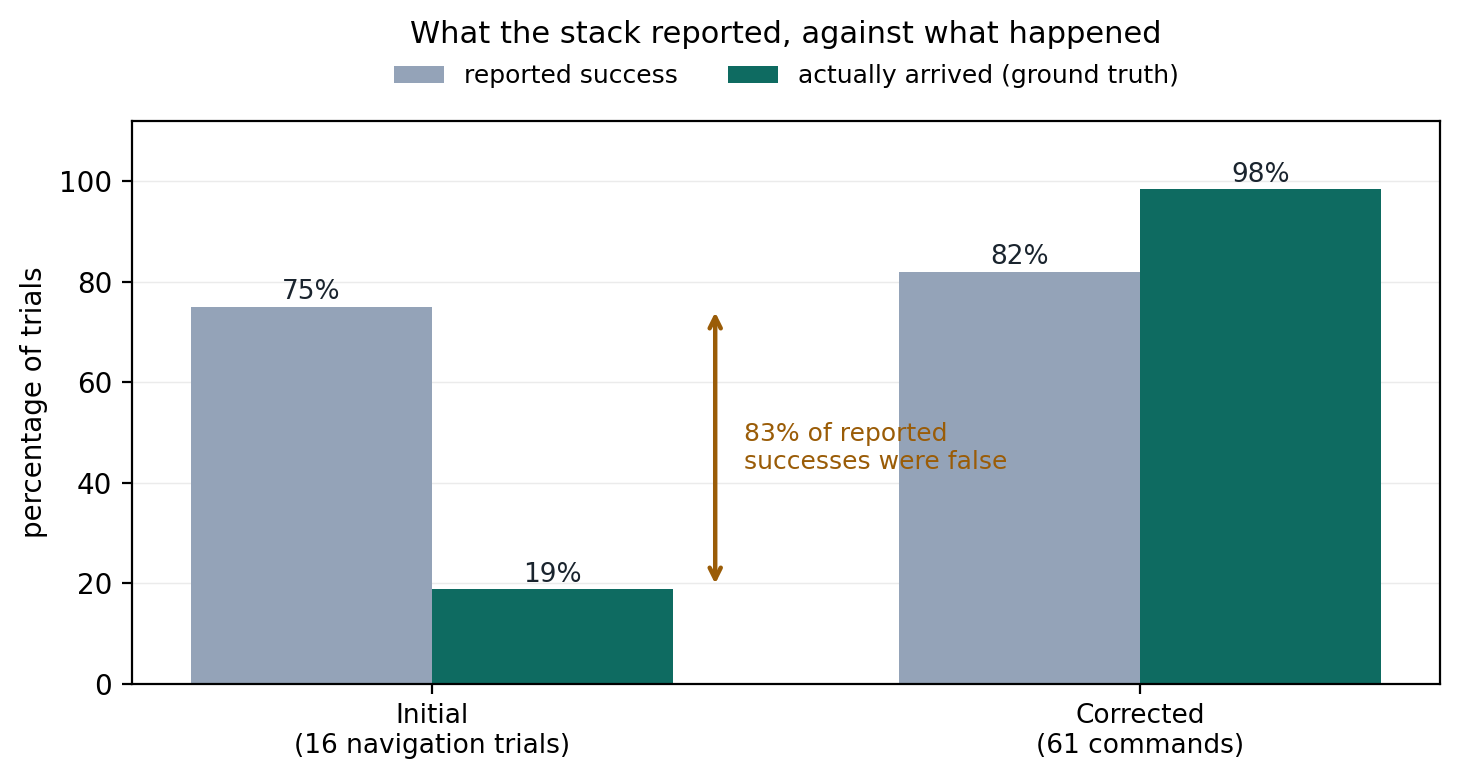
\includegraphics[width=\textwidth]{fig/reported_vs_actual.png}
\caption[Reported against actual]{The two runs on the same axes. Regenerate
with \file{scripts/plot\_validation.py}.}
\label{fig:repact}
\end{figure}

\begin{figure}[htbp]
\centering
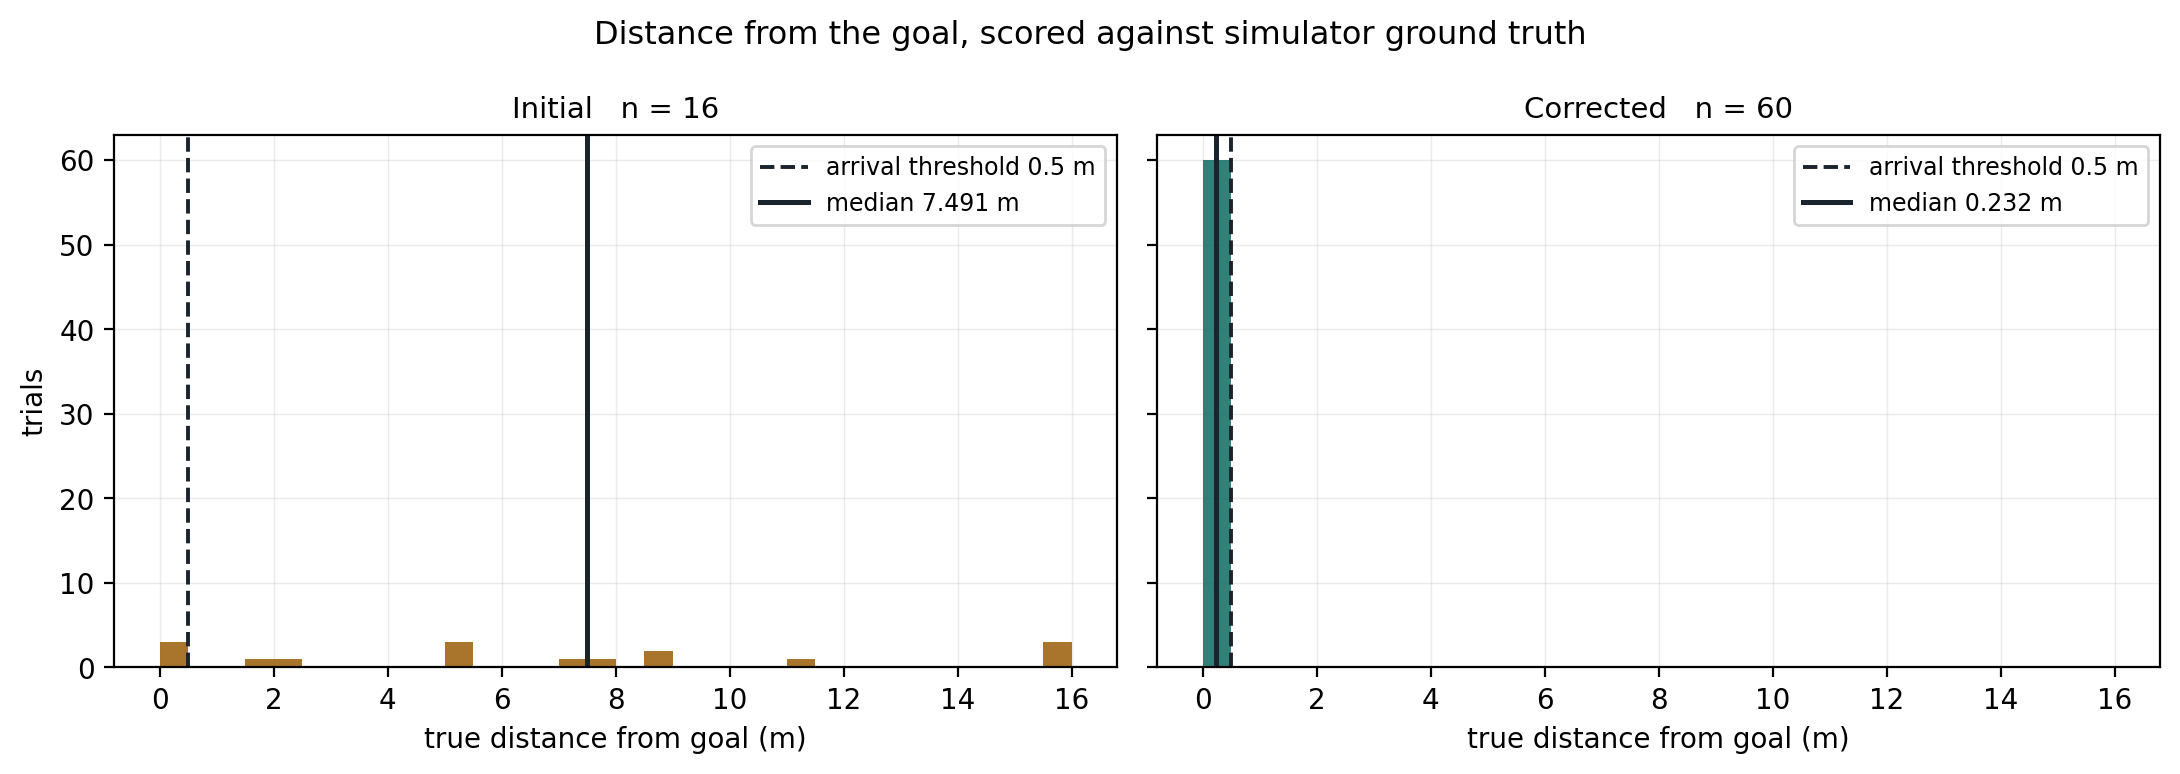
\includegraphics[width=\textwidth]{fig/error_dist.png}
\caption[Belief against truth]{Left: each trial placed at (error the robot
believed it had, error actually measured). Points on the diagonal are honest
beliefs; points high above it are the false positives. Right: how far the
estimate strayed, sorted. Regenerate with \file{scripts/plot\_validation.py}.}
\label{fig:errdist}
\end{figure}

\section{Table --- the ten unconfirmed arrivals}
\label{sec:hand-unconfirmed}

\begin{center}
\begin{tabular}{@{}lccc@{}}
\toprule
\textbf{Destination} & \textbf{Count} & $e_{\text{true}}$ \textbf{range (\si{\metre})} & \textbf{Duration (\si{\second})} \\
\midrule
\file{waiting\_area} & 4 & 0.12--0.23 & $\approx 185$ \\
\file{home}          & 3 & 0.22--0.30 & $\approx 185$ \\
\file{store\_area}   & 2 & 0.25--0.39 & 140--185 \\
\file{garage}        & 1 & 0.25       & 167 \\
\bottomrule
\end{tabular}
\end{center}

\begin{handbox}[The whole table, by hand]
Select rows of the corrected run where \file{outcome} is \emph{not}
\file{succeeded} but $e_{\text{true}} \le 0.5$. There are exactly ten:

\begin{center}
\small
\begin{tabular}{@{}rllrr@{}}
\toprule
$n$ & destination & outcome & $e_{\text{true}}$ & seconds \\
\midrule
 4 & home          & timeout & 0.287 & 184.8 \\
 8 & waiting\_area & timeout & 0.190 & 185.0 \\
10 & waiting\_area & timeout & 0.143 & 185.1 \\
11 & garage        & timeout & 0.252 & 167.4 \\
15 & home          & timeout & 0.222 & 184.9 \\
17 & waiting\_area & timeout & 0.230 & 185.4 \\
50 & home          & timeout & 0.298 & 184.8 \\
51 & store\_area   & timeout & 0.389 & 139.8 \\
54 & store\_area   & timeout & 0.249 & 184.8 \\
61 & waiting\_area & timeout & 0.117 & 185.2 \\
\bottomrule
\end{tabular}
\end{center}

Tally by destination: \file{waiting\_area} appears in rows $8, 10, 17, 61$ ---
\textbf{4}. \file{home} in rows $4, 15, 50$ --- \textbf{3}.
\file{store\_area} in rows $51, 54$ --- \textbf{2}. \file{garage} in row
$11$ --- \textbf{1}. Total $4+3+2+1 = 10$. \checkmark

Ranges: for \file{waiting\_area}, the smallest $e_{\text{true}}$ is $0.117$
and the largest is $0.230$, giving ``$0.12$--$0.23$''. \checkmark\;
For \file{home}: $0.222$ to $0.298$, giving ``$0.22$--$0.30$''. \checkmark

\medskip
\textbf{Three things fall out of this table immediately.}
\begin{enumerate}[leftmargin=1.6em,itemsep=2pt]
\item \emph{Every one is a} \file{timeout}, \emph{not an} \file{aborted}. The
navigation did not fail; it never finished.
\item \emph{Eight of the ten sat at almost exactly \SI{185}{\second}}, the
script's own timeout. They were still going when the clock ran out.
\item \emph{Every one of them was already there}, with errors between
\SI{0.117}{\metre} and \SI{0.389}{\metre} --- comfortably inside the
\SI{0.5}{\metre} arrival threshold, and mostly inside Nav2's own
\SI{0.25}{\metre} position tolerance.
\end{enumerate}
A robot that is at the goal, is not moving, and never finishes, is a robot
stuck on the \emph{heading} half of the goal check --- exactly the
translation-only progress-checker fault of Part~6~\S6.4.
\end{handbox}

\section{Numbers that cannot be done by hand --- and how they are obtained}

Three tables in the results require running something. Here is exactly what,
so the procedure is reproducible even though the arithmetic is not.

\subsection{Scan--map agreement}

\begin{center}
\begin{tabular}{@{}lc@{}}
\toprule
Mean distance to nearest wall & \SI{0.047}{\metre} \\
Median distance & \SI{0.050}{\metre} \\
Within \SI{0.10}{\metre} & $66.8\%$ \\
Within \SI{0.20}{\metre} & $100\%$ \\
\bottomrule
\end{tabular}
\end{center}

\begin{plain}[Procedure]
\begin{enumerate}[leftmargin=1.6em,itemsep=2pt]
\item Read the true pose $(t_x, t_y, t_\theta)$ from \file{gz model -m romr -p}.
\item Capture one message on \file{/scan}: $720$ ranges $z_k$ with angles
$\theta_k$.
\item For each beam, compute the point it hit, in map coordinates:
\[
p_k = \bigl(t_x + z_k \cos(t_\theta + \theta_k),\;\;
            t_y + z_k \sin(t_\theta + \theta_k)\bigr).
\]
\item Build a \term{distance transform} of the occupancy grid --- an image in
which every free cell holds its distance to the nearest occupied cell. This is
one call to \file{scipy.ndimage.distance\_transform\_edt} on the inverted map,
multiplied by the map resolution in metres per cell.
\item Look up each $p_k$ in that image. The result is $720$ distances.
\item Report their mean, median, and the fraction below each threshold.
\end{enumerate}
The rotation study repeats steps 3--6 with $t_\theta$ replaced by
$t_\theta + \Delta$ for $\Delta \in \{\ang{45}, \ang{90}, \ang{135}, \ang{180}\}$.

\smallskip
\textbf{Why you cannot do it by hand:} it is $720$ trigonometric evaluations
and $720$ image lookups per pose, times five poses. The arithmetic per beam is
trivial; the volume is not.
\end{plain}

\subsection{Localisation step response and the $\alpha$ sweep}

\begin{plain}[Procedure]
\begin{enumerate}[leftmargin=1.6em,itemsep=2pt]
\item Bring up the simulator and Nav2 (Part~10).
\item Seed AMCL from ground truth: \file{scripts/seed.sh}.
\item Read the baseline: true pose from \file{gz}, believed pose and
covariance from \file{/amcl\_pose}.
\item Apply \emph{one} isolated motion --- stand still \SI{8}{\second}, or
turn \ang{90}, or drive \SI{0.8}{\metre} --- using \file{scripts/drive.py}.
\item Read the three quantities again:
\[
e = \lVert \mathbf{b} - \mathbf{t}\rVert,\qquad
\Delta\theta = b_\theta - t_\theta,\qquad
\sigma_\theta = \sqrt{\Sigma_{\theta\theta}}
\]
where $\Sigma_{\theta\theta}$ is the yaw variance from the covariance matrix,
equation~\eqref{eq:cov}.
\item For the $\alpha$ sweep: edit \file{alpha1} and \file{alpha2} in
\file{config/nav2\_params.yaml}, restart Nav2, and repeat steps 2--5 for each
value $\{0.25, 0.10, 0.05, 0.02, 0.01\}$. \textbf{Re-seed before every trial},
or you are measuring accumulated history rather than the parameter.
\end{enumerate}
\textbf{Why you cannot do it by hand:} $\sigma_\theta$ is the spread over up to
$2000$ particles, each of which was moved by an independent random draw. There
is no closed form; it has to be run.
\end{plain}

\subsection{Goal reachability and costmap occupancy}

The claim that all eight destinations lie in one traversable region, with a
minimum clearance of \SI{1.09}{\metre}, and that $25.3\%$ of the costmap is at
or above the blocked value, comes from:

\begin{plain}[Procedure]
\begin{enumerate}[leftmargin=1.6em,itemsep=2pt]
\item Take the occupancy grid, threshold it into free / not-free.
\item Compute the distance transform (as above). Threshold it at the inscribed
radius \SI{0.229}{\metre}: cells with more clearance than that can hold the
robot.
\item Run a \term{connected-component} labelling over the result. Check that
all eight goal cells and the spawn cell carry the same label --- if they do,
they are mutually reachable.
\item The minimum clearance is the smallest distance-transform value among the
eight goal cells: \SI{1.09}{\metre}.
\item Subscribe to \file{/global\_costmap/costmap} and count cells at or above
the blocked value. \textbf{Remember the $0$--$100$ scale} (Part~6 \S6.3).
\end{enumerate}
\end{plain}

% =========================================================================
\chapter{Where everything lives}
\label{ch:files}

All paths are relative to the repository root,
\file{\raisebox{0pt}{\textasciitilde}/Multimodal-Robot-Autonomy}.

\section{Result files}

\begin{center}
\small
\begin{tabular}{@{}p{0.455\textwidth}p{0.495\textwidth}@{}}
\toprule
\textbf{Path} & \textbf{Contents} \\
\midrule
\file{validation\_results\_groundtruth.csv} &
  \textbf{The initial run.} 54 rows. The ``before'' column of every comparison. \\
\file{results/validation\_2026-08-04\_fixed.csv} &
  \textbf{The corrected run.} 61 rows. The ``after'' column. \\
\file{results/validation\_2026-08-04.csv} &
  An intermediate run: localisation fixed, navigation outcome identity not yet.
  57 aborts, 3 reported successes, all 3 genuine. Useful for showing the two
  faults were independent. \\
\file{validation\_results.csv} &
  An early \file{--mode chat} run without ground-truth columns. Superseded. \\
\midrule
\file{results/figures/reported\_vs\_actual.png} & Before/after on shared axes \\
\file{results/figures/error\_distribution.png} & Belief vs.\ truth scatter, and drift \\
\file{results/figures/alpha\_sweep.png} & The $\alpha_1$ sweep \\
\file{results/figures/graph\_trace.png} & One LangGraph run, traced \\
\file{results/particles\_*.png} & Particle clouds, tuned and mis-tuned \\
\file{results/particle\_approximation.png} & Density vs.\ particle representation \\
\file{results/urdf/} & Kinematic tree renderings of the ROMR description \\
\midrule
\file{backend/app/data/traces/graph\_runs.jsonl} &
  One JSON object per LangGraph run: nodes visited, timings, outcome \\
\bottomrule
\end{tabular}
\end{center}

\begin{warnbox}[A gotcha that cost real time]
Trace persistence writes to \file{backend/app/data/traces/}, resolved in code
as \file{Path(\_\_file\_\_).parents[1] / ``data'' / ``traces''}. It was briefly
\file{parents[2]}, which put the file in \file{backend/data/traces/} instead.
Because the write is best-effort and wrapped in a \file{try}, nothing ever
reported an error --- the traces simply were not where anything looked for
them. If a trace file seems empty, check both directories before assuming the
run failed.
\end{warnbox}

\section{Configuration}

\begin{center}
\small
\begin{tabular}{@{}p{0.455\textwidth}p{0.495\textwidth}@{}}
\toprule
\textbf{Path} & \textbf{Contents} \\
\midrule
\file{config/nav2\_params.yaml} &
  \textbf{The central file of this study.} AMCL, planner, controller,
  costmaps, recoveries. Heavily commented with the measurement behind each
  value. \\
\file{config/cyclonedds.xml} &
  Pins DDS discovery to unicast loopback. Not optional on this host --- see
  Part~10 \S10.1. \\
\file{backend/app/data/places/} \newline \file{\ \ \ \ new\_world\_places.yaml} &
  The eight destinations and their aliases. Goal coordinates come from here. \\
\file{backend/.env} &
  API keys and model selection (\file{gpt-4.1-mini}). Never committed. \\
\midrule
\file{\$WS/src/romr\_description/} \newline \file{\ \ \ \ urdf/} & The robot description \\
\file{\$WS/src/} \newline \file{\ \ \ \ multimodal\_robot\_autonomy/} \newline \file{\ \ \ \ \ \ \ \ gazebo/} &
  Gazebo plugins: differential drive, laser, camera, IMU. Here
  \file{\$WS} is \file{\raisebox{0pt}{\textasciitilde}/turtlebot3\_ws} \\
\bottomrule
\end{tabular}
\end{center}

\section{Scripts}

\begin{center}
\small
\begin{tabular}{@{}p{0.34\textwidth}p{0.60\textwidth}@{}}
\toprule
\textbf{Script} & \textbf{Purpose} \\
\midrule
\file{scripts/env.sh} & Shared environment. \emph{Source} it, do not run it. \\
\file{scripts/build.sh} & Rebuild into \file{\raisebox{0pt}{\textasciitilde}/turtlebot3\_ws} --- the workspace that is
   actually sourced \\
\file{scripts/clean.sh} & Kill every leftover process. Run before every session \\
\midrule
\file{scripts/sim.sh} & Terminal 1: Gazebo, world, robot \\
\file{scripts/nav2\_rviz.sh} & Terminal 2: Nav2 with RViz \\
\file{scripts/backend.sh} & Terminal 3: FastAPI on \file{:8000} \\
\file{scripts/frontend.sh} & Terminal 4: Next.js on \file{:3000} \\
\midrule
\file{scripts/seed.sh} & Seed AMCL from Gazebo ground truth, then rotate to converge \\
\file{scripts/drive.sh} & Arrow-key teleoperation \\
\file{scripts/record\_place.py} & Record the current pose as a named destination \\
\file{scripts/watch.sh} & Live readout of truth, belief, drift and $\sigma$ \\
\midrule
\file{scripts/validate\_commands.py} & \textbf{The evaluation suite.} Produces the CSVs \\
\file{scripts/plot\_validation.py} & Belief-vs-truth scatter and drift plot \\
\file{scripts/plot\_results.py} & The $\alpha$ sweep and before/after figures \\
\file{scripts/plot\_trace.py} & LangGraph trace figure \\
\file{scripts/particle\_figure.py} & Particle-cloud figures \\
\midrule
\file{scripts/map\_world.sh}, \file{scripts/save\_map.sh} & SLAM and map capture \\
\file{scripts/record\_screen.sh} & Screen capture for the demonstration \\
\bottomrule
\end{tabular}
\end{center}

\section{Backend code that matters to this document}

\begin{center}
\small
\begin{tabular}{@{}p{0.455\textwidth}p{0.495\textwidth}@{}}
\toprule
\textbf{Path} & \textbf{Role} \\
\midrule
\file{backend/app/services/ros2\_bridge.py} &
  The ROS~2 side: subscribes \file{/amcl\_pose} (transient-local), \file{/scan},
  the camera; dispatches \file{NavigateToPose}; holds the goal-epoch mechanism \\
\file{backend/app/services/command\_graph.py} &
  The LangGraph state machine of Figure~\ref{fig:langgraph} \\
\file{backend/app/services/intent\_parser.py} &
  Utterance $\rightarrow$ intent $+$ place \\
\file{backend/app/services/vector\_store.py} &
  \file{VectorStore} protocol with Chroma and Pinecone backends. Chroma
  returns a \emph{distance}, Pinecone a \emph{similarity}; the adapter converts
  with \file{score = 1.0 - distance} so ranking is not silently inverted \\
\file{backend/app/core/security.py} &
  Rate limiting; \file{is\_local()} exempts loopback \\
\bottomrule
\end{tabular}
\end{center}

% =========================================================================
\chapter{Running it: from a cold machine to a results CSV}
\label{ch:run}

\section{Two settings that are not optional on this host}

Before anything else, understand why \file{scripts/env.sh} exists. Two
environment settings must be right or the stack will appear to work while
delivering nothing.

\begin{plain}[The DDS problem]
ROS~2 nodes find each other by multicast discovery. \textbf{This host has no
multicast route}, and the default domain (0) collides with another machine on
the network. The symptoms are maddening: \file{ros2 topic list} shows the
topics, \file{ros2 topic echo} shows nothing, and every node reports itself
healthy.

Two settings fix it, both applied by \file{env.sh}:
\begin{center}
\file{export CYCLONEDDS\_URI="file://\$REPO/config/cyclonedds.xml"} \\
\file{export ROS\_DOMAIN\_ID=42}
\end{center}
The XML pins discovery to unicast loopback. The domain ID keeps this stack off
the contended default.

\smallskip
\file{env.sh} also unsets the \file{SNAP\_*}, \file{GTK\_PATH} and
\file{LD\_LIBRARY\_PATH} variables that VS Code's snap injects, which otherwise
kill \file{rviz2} and \file{gz} with
\file{undefined symbol: \_\_libc\_pthread\_init}; and it detects the actual
X display rather than assuming \file{:0}, because this machine runs on
\file{:1}.
\end{plain}

\section{Start from a clean slate --- always}

\begin{plain}[Terminal 0]
\begin{verbatim}
cd ~/Multimodal-Robot-Autonomy
scripts/clean.sh          # simulator, nav2, rviz
scripts/clean.sh --all    # ... and the backend (:8000) and frontend (:3000)
\end{verbatim}
It prints \file{clean: nothing left running} when the slate is genuinely clear.
\end{plain}

\begin{warnbox}[The single most common failure in this project is not a bug]
It is a stale process. Three specific ones, each of which produces symptoms
that look exactly like an application fault:

\begin{enumerate}[leftmargin=1.6em,itemsep=3pt]
\item \textbf{A forgotten \file{teleop\_twist\_keyboard}.} It republishes its
last twist in a loop, so a session left open after one keypress drives the
robot forever. Measured: \SI{588}{\milli\metre} of creep in \SI{60}{\second}
with nobody touching the keyboard. This reads exactly like a physics bug and is
not one.

\item \textbf{Extra \file{robot\_state\_publisher} processes.} Each publishes
its own \file{/robot\_description} and TF, so a stale robot model keeps being
spawned after the URDF has changed. Twenty-two of them accumulated here,
because \file{pkill -x a b c} does \emph{not} kill \file{a}, \file{b} and
\file{c} --- it takes one pattern and rejects the rest. \file{clean.sh} calls
\file{pkill} once per process name for exactly this reason.

\item \textbf{\file{slam\_toolbox} outliving its launch file.} It keeps
publishing \file{map}$\rightarrow$\file{odom}, silently fighting AMCL for the
same transform the next time Nav2 comes up. Two nodes publishing the same
transform is undefined behaviour, and the resulting pose jitters between them.
\end{enumerate}

Note also the bracket idiom throughout \file{clean.sh}:
\file{pkill -f "[g]azebo\_romr.launch.py"}. The brackets stop the pattern from
matching \file{pkill}'s own command line, which would make the script kill the
shell that launched it.
\end{warnbox}

\section{The five terminals}

\begin{plain}[Bring-up, in order]
\begin{verbatim}
# Terminal 1 - simulator, world and robot
scripts/sim.sh

# Terminal 2 - navigation with RViz, so the initial pose can be set by hand
scripts/nav2_rviz.sh

# Terminal 3 - reasoning backend, FastAPI on :8000
scripts/backend.sh

# Terminal 4 - command centre, Next.js on :3000
scripts/frontend.sh

# Terminal 5 - working shell for seeding, driving and validation
source scripts/env.sh
\end{verbatim}
Wait for each to settle before starting the next. Terminal 2 in particular
should be given time to report all its lifecycle nodes active.
\end{plain}

\begin{plain}[If a newly added file seems to be ignored]
Rebuild --- but with the right script:
\begin{verbatim}
scripts/build.sh
\end{verbatim}
The package \emph{source} lives in this repository, but the colcon workspace is
\file{\raisebox{0pt}{\textasciitilde}/turtlebot3\_ws}, which carries this directory as a symlink under
\file{src/} and is what \file{env.sh} sources. Running \file{colcon build} from
the repository root succeeds, prints no warning, and creates a second install
tree that nothing ever reads.

Existing files survive that mistake, because \file{--symlink-install} links
them back to source. \emph{New} files do not: they are only linked at build
time, so a newly added launch file, RViz config or map is simply absent and the
tool that wanted it falls back to a default instead of reporting the miss. A
brand-new \file{navigation.rviz} was silently replaced by RViz's factory layout
exactly this way.
\end{plain}

\section{Localise the robot}

AMCL starts with \file{set\_initial\_pose: false}, so until it is told where the
robot is it publishes no \file{map}$\rightarrow$\file{odom} transform and every
goal fails to plan. Two ways to fix that:

\begin{enumerate}[leftmargin=1.6em,itemsep=3pt]
\item \textbf{By hand, in RViz.} Click \textbf{2D Pose Estimate}, then click
where the robot is and drag in the direction it faces.
\item \textbf{From ground truth.}
\begin{verbatim}
scripts/seed.sh
\end{verbatim}
This reads the true pose from Gazebo, publishes it on \file{/initialpose},
\emph{and then rotates the robot in place}.
\end{enumerate}

\begin{keyidea}[Why \file{seed.sh} rotates afterwards, and why that is not cheating]
A particle filter only updates when the robot has moved past
\file{update\_min\_d} (\SI{0.25}{\metre}) or \file{update\_min\_a}
(\SI{0.2}{\radian}). A stationary robot therefore keeps whatever spread it was
seeded with forever --- the initial cloud is never corrected by a scan, because
no update ever fires. Rotating in place is the cheapest way to force updates
and cannot collide with anything.

This is a legitimate initialisation, not a thumb on the scale, and it is
reported: the validation script counts every re-seed and prints the total. In
the corrected run that total is $0/61$.
\end{keyidea}

\section{Watch what is happening}

\begin{plain}[Terminal 5]
\begin{verbatim}
scripts/watch.sh
\end{verbatim}
prints, live: the true pose from Gazebo, the believed pose from
\file{/amcl\_pose}, the gap between them, and $\sigma_x$, $\sigma_y$,
$\sigma_\theta$. This is the same triple that
equation~\eqref{eq:threedist} scores, shown continuously.

Read the ground truth directly at any time with:
\begin{verbatim}
gz model -m romr -p
\end{verbatim}
\end{plain}

\section{Run the evaluation}

\begin{plain}[The suite]
\begin{verbatim}
# quick smoke test - eight commands
scripts/validate_commands.py --mode graph --limit 8

# the full suite
OUT=results/validation_$(date +%F).csv
scripts/validate_commands.py --mode graph --out $OUT
\end{verbatim}

Options:
\begin{center}
\small
\begin{tabular}{@{}lp{0.19\textwidth}p{0.50\textwidth}@{}}
\toprule
\textbf{Flag} & \textbf{Default} & \textbf{Meaning} \\
\midrule
\file{--mode} & \file{graph} & \file{graph} waits for the real navigation
   outcome and retries once with costmaps cleared; \file{chat} only dispatches \\
\file{--out} & {\scriptsize\texttt{validation\_\newline results.csv}} & output path \\
\file{--limit} & 0 (all) & run only the first $N$ trials \\
\file{--timeout} & \SI{300}{\second} & HTTP timeout per command \\
\file{--seed} & 7 & shuffle seed, so trial order is reproducible \\
\file{--settle} & \SI{3}{\second} & pause between trials \\
\file{--arrival-tol} & \SI{0.5}{\metre} & the threshold of Part~7 \S7.3 \\
\bottomrule
\end{tabular}
\end{center}

Requirements: the simulator, Nav2 and the backend must be up, and \file{gz}
must be on \file{PATH} --- without it there is no ground truth and the
\file{error\_true\_m} column will be empty, which silently reduces the study to
the very self-assessment it was designed to avoid. \textbf{Check that column is
populated before trusting a run.}
\end{plain}

\section{Produce the figures}

\begin{plain}
\begin{verbatim}
scripts/plot_validation.py results/validation_2026-08-04_fixed.csv \
                          results/figures/error_distribution.png
scripts/plot_results.py
scripts/plot_trace.py
scripts/particle_figure.py
\end{verbatim}
\end{plain}

\section{Adding or moving a destination}

\begin{plain}
Drive the robot to the spot, point it the way it should end up facing, then:
\begin{verbatim}
scripts/record_place.py garage
scripts/record_place.py parlour --alias "living room" --alias lounge
scripts/record_place.py --list
scripts/record_place.py --check     # audit every place against the map
\end{verbatim}
The pose is taken from TF \file{map}$\rightarrow$\file{base\_link}, because
that is the frame Nav2 plans in and therefore the only frame in which a goal
means anything. Gazebo's ground truth is read as well, purely to report the
gap: if localisation is off when you record a place, you bake that error
permanently into the registry, and every future trial to that destination
inherits it.
\end{plain}

% =========================================================================
\chapter{What was tuned, and what is left}
\label{ch:tuning}

\section{The four faults that were fixed}

Each fault is classified by which side of the importance-sampling
identity~\eqref{eq:importance} it sat on --- a distinction that determines how
seriously to take it.

\begin{center}
\small
\begin{tabular}{@{}p{0.20\textwidth}p{0.09\textwidth}p{0.20\textwidth}p{0.40\textwidth}@{}}
\toprule
\textbf{Fault} & \textbf{Half} & \textbf{Was} $\rightarrow$ \textbf{Is} & \textbf{Exposed by} \\
\midrule
Sensor range cutoff & weight &
  \SI{8}{\metre} $\rightarrow$ \SI{16}{\metre} &
  The fitted scanner reaches \SI{16}{\metre} in a \SI{13.85}{\metre} building \\
Rotational noise coefficient & proposal &
  $0.20$, then $0.25$ $\rightarrow$ $0.02$ &
  The sweep of Part~5 \S5.3 \\
Hit-vs-noise weighting & weight &
  $0.5/0.5$ $\rightarrow$ $0.8/0.2$ &
  Scan--map agreement, Part~5 \S5.4 \\
Navigation outcome identity & --- &
  untagged $\rightarrow$ per-goal epoch &
  The duration audit of Part~8 \S8.3 \\
\bottomrule
\end{tabular}
\end{center}

\begin{keyidea}[Why the classification matters]
A \textbf{proposal} fault degrades the estimator while still targeting the
right posterior --- it makes the filter inefficient. A \textbf{weight} fault
changes \emph{what is being estimated} --- the filter converges confidently on
the answer to a different question.

Two of the three model faults here were weight faults. That is consistent with
what was observed: not a noisy estimate, but a confident and wrong one. It also
means the fix could not have come from adding particles, adding compute, or
waiting longer.
\end{keyidea}

\section{Tuning levers not yet exhausted}

Each entry below states the current value, a candidate, the mechanism by which
it should help, how to measure whether it did, and the risk of doing it.
Nothing here is a recommendation to change blindly --- the lesson of Part~5
\S5.3 is precisely that plausible reasoning about these parameters can point
the wrong way, and only a sweep settles it.

\subsection{Lever 1 --- the progress checker (highest expected value)}

\begin{center}
\small
\begin{tabular}{@{}p{0.20\textwidth}p{0.74\textwidth}@{}}
\toprule
\textbf{Current} & \file{SimpleProgressChecker}, \file{required\_movement\_radius: 0.3},
  \file{movement\_time\_allowance: 10.0} \\
\textbf{Candidates} & (a) \file{PoseProgressChecker}, which counts rotation as
  progress; (b) keep \file{SimpleProgressChecker} but raise
  \file{movement\_time\_allowance} above the worst observed final-rotation time;
  (c) relax \file{yaw\_goal\_tolerance} from \SI{0.25}{\radian} to
  \SI{0.5}{\radian} \\
\textbf{Mechanism} & Part~6 \S6.4: the checker measures translation only, so a
  robot rotating on the spot at the goal registers no progress and is aborted \\
\textbf{Expected effect} & Recall $0.833 \rightarrow$ close to $1.000$;
  precision should stay at $1.000$ because these trials genuinely arrived \\
\textbf{Measurement} & Re-run the full suite; count rows with
  \file{outcome != succeeded} and $e_{\text{true}} \le 0.5$. Target: zero \\
\textbf{Risk} & (a) and (b) both weaken the stack's ability to detect a
  genuinely stuck robot --- a robot spinning uselessly against a wall would now
  be tolerated for longer. (c) weakens the arrival criterion itself, which
  trades a reporting defect for a quality one. \textbf{(a) was trialled during
  this project and reverted}; if it is revisited, the \emph{stuck} case must be
  tested explicitly, not just the arrival case \\
\bottomrule
\end{tabular}
\end{center}

\subsection{Lever 2 --- resampling interval}

\begin{center}
\small
\begin{tabular}{@{}p{0.20\textwidth}p{0.74\textwidth}@{}}
\toprule
\textbf{Current} & \file{resample\_interval: 1} --- resample on every update \\
\textbf{Candidate} & $2$ or $3$ \\
\textbf{Mechanism} & Part~4: AMCL uses multinomial resampling, which has no
  survival guarantee and count variance growing with $J$
  (equation~\eqref{eq:multivar}). Resampling less often lets weights accumulate
  information across several scans before diversity is spent \\
\textbf{Measurement} & Repeat the step-response protocol of Part~8 \S8.10.2 and
  watch $\sigma_\theta$ after a \ang{90} turn. Also log the
  \term{effective sample size} $\;J_{\text{eff}} = 1 / \sum_j (w^{[j]})^2$;
  the standard rule is to resample only when $J_{\text{eff}} < J/2$ \\
\textbf{Risk} & Weight degeneracy in the other direction: if resampling is too
  rare, one particle takes all the weight and the filter is effectively running
  on a single hypothesis \\
\bottomrule
\end{tabular}
\end{center}

\subsection{Lever 3 --- update thresholds during rotation}

\begin{center}
\small
\begin{tabular}{@{}p{0.20\textwidth}p{0.74\textwidth}@{}}
\toprule
\textbf{Current} & \file{update\_min\_d: 0.25}, \file{update\_min\_a: 0.2} (\ang{11.5}) \\
\textbf{Candidate} & \file{update\_min\_a: 0.1} (\ang{5.7}), leaving
  \file{update\_min\_d} alone \\
\textbf{Mechanism} & Every measurement in this project says rotation is where
  the error enters and translation is benign --- Part~2 \S2.3.1. Correcting
  twice as often \emph{during} the motion that causes the damage attacks the
  problem where it happens, rather than after \\
\textbf{Measurement} & Step response after a \ang{90} turn: $e$,
  $\Delta\theta$, $\sigma_\theta$. Also record CPU load, since this doubles the
  filter rate during turns \\
\textbf{Risk} & More frequent updates mean more frequent resampling, which
  interacts with Lever 2. Change one at a time \\
\bottomrule
\end{tabular}
\end{center}

\subsection{Lever 4 --- sharpening the likelihood}

\begin{center}
\small
\begin{tabular}{@{}p{0.20\textwidth}p{0.74\textwidth}@{}}
\toprule
\textbf{Current} & \file{sigma\_hit: 0.2}, \file{max\_beams: 120}, \file{z\_hit: 0.8} \\
\textbf{Candidates} & \file{sigma\_hit: 0.1}; \file{max\_beams: 180} \\
\textbf{Mechanism} & The measured mean beam-to-wall distance at the true pose is
  \SI{0.047}{\metre} and the median \SI{0.050}{\metre} --- both well inside the
  current $\sigma_{\text{hit}} = \SI{0.2}{\metre}$. A Gaussian four times wider
  than the actual residual is a blunt instrument: it scores a pose
  \SI{15}{\centi\metre} wrong almost as highly as the correct one. Halving it
  sharpens the peak in equation~\eqref{eq:phit} \\
\textbf{Measurement} & The rotation study of Part~8 \S8.10.1: recompute mean
  agreement at $\Delta = 0$ against $\ang{45}, \ang{90}, \ang{135}, \ang{180}$
  and check the contrast \emph{ratio} improves, not just the absolute value \\
\textbf{Risk} & Real. A too-narrow $\sigma_{\text{hit}}$ makes the likelihood
  so peaked that no particle scores well, weights collapse toward zero, and the
  filter loses track after a single unmodelled disturbance. \SI{0.047}{\metre}
  is the residual \emph{when correctly localised}; the filter also has to score
  poses that are slightly wrong, and it needs to be able to grade them. Sweep
  it; do not jump \\
\bottomrule
\end{tabular}
\end{center}

\subsection{Lever 5 --- using the covariance as a gate}

\begin{center}
\small
\begin{tabular}{@{}p{0.20\textwidth}p{0.74\textwidth}@{}}
\toprule
\textbf{Current} & $\sigma_x$, $\sigma_y$, $\sigma_\theta$ are logged by
  \file{belief()} in the validation script but not acted on \\
\textbf{Candidate} & Refuse to report success, or trigger a re-localisation,
  when $\sigma_{\text{pos}} = \sqrt{\sigma_x^2 + \sigma_y^2}$ exceeds a
  threshold \\
\textbf{Mechanism} & Ground truth exists here and does not exist on a real
  vehicle. A self-assessment that predicts true error is the only signal that
  could carry this decision in deployment \\
\textbf{Measurement} & \textbf{This is a study, not a setting.} Plot
  $\sigma_{\text{pos}}$ against $e_{\text{true}}$ across the suite and compute
  the correlation. If they are uncorrelated, the covariance is useless as a
  gate and \emph{that is a publishable negative result} \\
\textbf{Risk / caveat} & The corrected run has almost no spread in
  $e_{\text{true}}$ (everything between $0.117$ and $0.483$), so there is
  nothing for $\sigma$ to correlate \emph{with}. The study needs deliberately
  induced failures --- restore \file{laser\_max\_range: 8.0}, or raise
  $\alpha_1$ --- to generate the range. Part~5 \S5.7 already warns that
  $\Sigma$ measures particle agreement, not correctness, so the honest prior is
  that this will correlate weakly \\
\bottomrule
\end{tabular}
\end{center}

\subsection{Lever 6 --- inflation, currently uncommitted}

\begin{center}
\small
\begin{tabular}{@{}p{0.20\textwidth}p{0.74\textwidth}@{}}
\toprule
\textbf{Current} & \file{cost\_scaling\_factor: 6.0}, \file{inflation\_radius: 0.55}
  --- present in the working tree but not committed \\
\textbf{Mechanism} & Equation~\eqref{eq:inflation}. A larger radius or a
  smaller scaling factor pushes paths further from walls, at the cost of
  refusing narrow doorways \\
\textbf{Measurement} & Two numbers together, never one: the fraction of the
  global costmap at or above the blocked value (currently $25.3\%$), and the
  planner's success rate over all eight destinations from all eight starts \\
\textbf{Risk} & This interacts directly with localisation. A wider inflation
  makes the ``believed pose lands in an inflated cell, planner refuses every
  goal'' cascade of Part~7 \S7.5 trigger at a smaller drift. Tuning inflation
  up to compensate for localisation error is treating the symptom \\
\bottomrule
\end{tabular}
\end{center}

\subsection{Lever 7 --- the resampler itself}

\begin{center}
\small
\begin{tabular}{@{}p{0.20\textwidth}p{0.74\textwidth}@{}}
\toprule
\textbf{Current} & Multinomial, fixed inside \file{nav2\_amcl}, not configurable \\
\textbf{Candidate} & Fork \file{nav2\_amcl} and implement stochastic universal
  sampling, accepting a fixed $J$ in place of KLD adaptation \\
\textbf{Mechanism} & Part~4 \S4.3.2--4.3.3: bounded count variance and a hard
  survival guarantee for any particle with $w \ge 1/J$ \\
\textbf{Measurement} & With $J$ fixed at $2000$ for both arms, compare
  $\sigma_\theta$ after a \ang{90} turn, and the number of distinct ancestors
  surviving after $50$ updates \\
\textbf{Risk} & High effort, and it discards KLD adaptation --- the filter
  would carry $2000$ particles even when converged. \textbf{This is a
  legitimate piece of future work and should be described as such, not
  attempted late.} It is also the only item in this list that changes code
  outside this repository \\
\bottomrule
\end{tabular}
\end{center}

\section{A protocol for tuning anything on this list}

\begin{plain}[Five rules, learned the hard way in this project]
\begin{enumerate}[leftmargin=1.6em,itemsep=4pt]
\item \textbf{Change one parameter at a time.} Two of the four faults above
were found only because they were isolated. The intermediate run
(\file{results/validation\_2026-08-04.csv}) exists precisely to show the
localisation fix and the outcome-identity fix were independent.

\item \textbf{Re-seed before every trial.} Otherwise you measure accumulated
history rather than the parameter. \file{scripts/seed.sh}.

\item \textbf{Sweep, do not reason.} $\alpha_1 = 0.25$ was chosen by a
physically correct argument about caster scrub and is the worst point on the
curve. The parameter's units --- variance per unit motion squared --- do not
match the intuition the argument appeals to.

\item \textbf{Score against ground truth, never against the estimate.}
\file{gz model -m romr -p}. Anything else measures the robot's opinion of
itself.

\item \textbf{Report the negative results.} The recovery-alpha experiment, the
$\alpha_1 = 0.25$ trial and the reverted progress checker are all more
informative than the settings that happened to work, because they say
\emph{why} the working settings work.
\end{enumerate}
\end{plain}

% =========================================================================
\chapter{Glossary}
\label{ch:glossary}

\begin{longtable}{@{}p{0.26\textwidth}p{0.70\textwidth}@{}}
\toprule
\textbf{Term} & \textbf{Meaning} \\
\midrule
\endhead
AMCL & Adaptive Monte Carlo Localisation. A particle filter that estimates the
  robot's pose in a known map, with the number of particles adapting to how
  uncertain it is. \\
Bayes' rule & $P(A\mid B) = P(B\mid A)P(A)/P(B)$. The formula for updating a
  belief when evidence arrives. Equation~\eqref{eq:bayes}. \\
Belief & The full probability density over where the robot might be, not a
  single position. Equation~\eqref{eq:belief}. \\
Costmap & A grid over the environment where each cell holds how bad it is to be
  there. Published on a $0$--$100$ scale. \\
Covariance & A matrix describing how spread out the particles are, and how
  their errors correlate. Equation~\eqref{eq:cov}. \\
Dead reckoning & Estimating position by adding up small movements. Never
  self-corrects. Equation~\eqref{eq:deadreckon}. \\
Density & A function whose \emph{area} over an interval gives a probability.
  Can exceed $1$; the total area is always $1$. \\
Drift & Here, $d_{\text{drift}}$: the gap between where the robot believes it
  is and where it actually is. \\
DWB & Dynamic Window Approach local planner. Simulates a fan of short
  trajectories each cycle and picks the best-scoring one. \\
Expected value & The average of a quantity under a density. An integral,
  equation~\eqref{eq:expectation}. \\
False positive & The stack reported success and the robot had not arrived. The
  central quantity of this study. \\
Footprint & The robot's outline as a polygon, rather than a single radius.
  ROMR: \SI{0.521}{\metre} by \SI{0.608}{\metre}. \\
Frame & An origin and set of axes. This project uses \file{map}, \file{odom}
  and \file{base\_link}. \\
Ground truth & The real answer, obtained independently of the system under
  test. Here: \file{gz model -m romr -p}. \\
Importance sampling & Sampling from a convenient density and correcting with
  weights. Equation~\eqref{eq:importance}. \\
Inflation & A soft cost halo painted around obstacles so paths avoid hugging
  walls. Equation~\eqref{eq:inflation}. \\
Integral & An area under a curve; equivalently, a total made of infinitely many
  infinitely small pieces. \\
KLD sampling & The rule that decides how many particles AMCL needs, from how
  spread out they currently are. Equation~\eqref{eq:kld}. \\
Likelihood & How plausible the observed sensor reading is, supposing a
  particular pose. Equations~\eqref{eq:beammix}--\eqref{eq:phit}. \\
Mean / median & Average / middle value. The results report both, because they
  differ when there are outliers. \\
Multinomial resampling & The roulette-wheel method: $J$ independent draws.
  What \file{nav2\_amcl} uses. Part~4 \S4.2. \\
Nav2 & The ROS~2 navigation stack: planner, controller, recoveries, behaviour
  tree. \\
Normalisation & Dividing by a total so probabilities sum (or integrate) to $1$.
  Equation~\eqref{eq:normalise}. \\
Odometry & Position estimated from wheel rotation. Smooth but drifting. \\
Particle & One complete hypothesis about the pose: an $(x, y, \theta)$ triple
  plus a weight. \\
Particle depletion & Loss of diversity through repeated resampling, until every
  particle descends from one ancestor. \\
Posterior / prior & Belief after / before the evidence. \\
Precision / recall & Of the claims made, how many were true / of the
  opportunities, how many were claimed. Part~8 \S8.8. \\
Proposal & The density you actually sample from, $\pi$. A design choice. \\
Resampling & Replacing the weighted particle set with an equally weighted one
  by drawing with replacement. \\
Standard deviation ($\sigma$) & Square root of variance; typical distance from
  the mean, in the original units. \\
Stochastic universal sampling & The comb method: one random offset, $J$ equally
  spaced pointers. Lower variance, $O(J)$, unused by AMCL. Part~4 \S4.3. \\
Support condition & The requirement that the proposal can generate samples
  everywhere the truth might be. Equation~\eqref{eq:support}. \\
TF & The ROS transform system. The seam through which AMCL's answer reaches
  Nav2, carrying no confidence with it. \\
Variance & Mean squared distance from the mean. Measures spread. \\
Weight & A particle's share of the belief; in importance sampling,
  $w = p / \pi$. Forced, not chosen. \\
\bottomrule
\end{longtable}

\chapter*{Sources for the reproduced material}
\addcontentsline{toc}{chapter}{Sources for the reproduced material}
\markboth{Sources}{}

Two items in this document are not original to the project and must be cited
wherever they are reused.

\begin{enumerate}[leftmargin=1.6em,itemsep=5pt]
\item \textbf{Figure~\ref{fig:nav2arch}, the Navigation~2 architecture
diagram}, is reproduced from the Navigation~2 documentation. Cite
Macenski~et~al., \emph{The Marathon 2: A Navigation System}, IROS 2020, and the
Navigation~2 documentation at \url{https://docs.nav2.org}.

\item \textbf{The source excerpts in Part~4 \S4.4} are quoted from
\file{nav2\_amcl/src/pf/pf.c} on the \texttt{humble} branch of
\url{https://github.com/ros-navigation/navigation2}. The particle-filter
implementation descends from the Player/Stage project and carries its original
authorship; the KLD sampling rule of equation~\eqref{eq:kld} is due to Fox,
\emph{KLD-Sampling: Adaptive Particle Filters}, NIPS 2001.
\end{enumerate}

\noindent The standard reference for Parts~1--5 is Thrun, Burgard and Fox,
\emph{Probabilistic Robotics} (MIT Press, 2005): Chapter~2 for the Bayes
filter, Chapter~4 for particle filters and resampling, Chapter~5 for the
motion models and the $\alpha$ coefficients, Chapter~6 for the beam and
likelihood-field measurement models, and Chapter~8 for Monte Carlo
localisation.

\medskip
\noindent All measurements, all tables, all CSV files and every other figure in
this document were produced by this project, in simulation.

\end{document}
